\chapter{Konzeption des Metamodells}

\section{Konzeptionelle Rahmenbedingungen}

\subsection{Anforderungen an eine Lösung / Vorrausetzungen / Methodik / Bewertungskriterien}

Das Microservice-Architekturmuster fordert eine technologisch unabhängige Implementierung. Aus Gründen der Einfachheit werden in dieser Arbeit die Zieltechnologien im Kontext der Generierung auf einzelne Technologien beschränkt. Trotzdem soll im Metamodell die Möglichkeit, andere Zieltechnologien zu haben, berücksichtigt werden.

\subsection{Einbindung aktueller Technologien}

Da verschiedene Ansätze zur modellgetriebenen Entwicklung von Microservices existieren, werden im Folgenden verschiedene Lösungen näher betrachtet. Dabei werden die grundlegenden Ansätze analysiert, Stärken und Schwächen differenziert betrachtet und die Möglichkeiten einer Integration in eine Lösung zur Zielstellung dieser Arbeit bewertet.

\subsubsection{AjiL}

%TODO GitHub Quelle angeben
\begin{center}
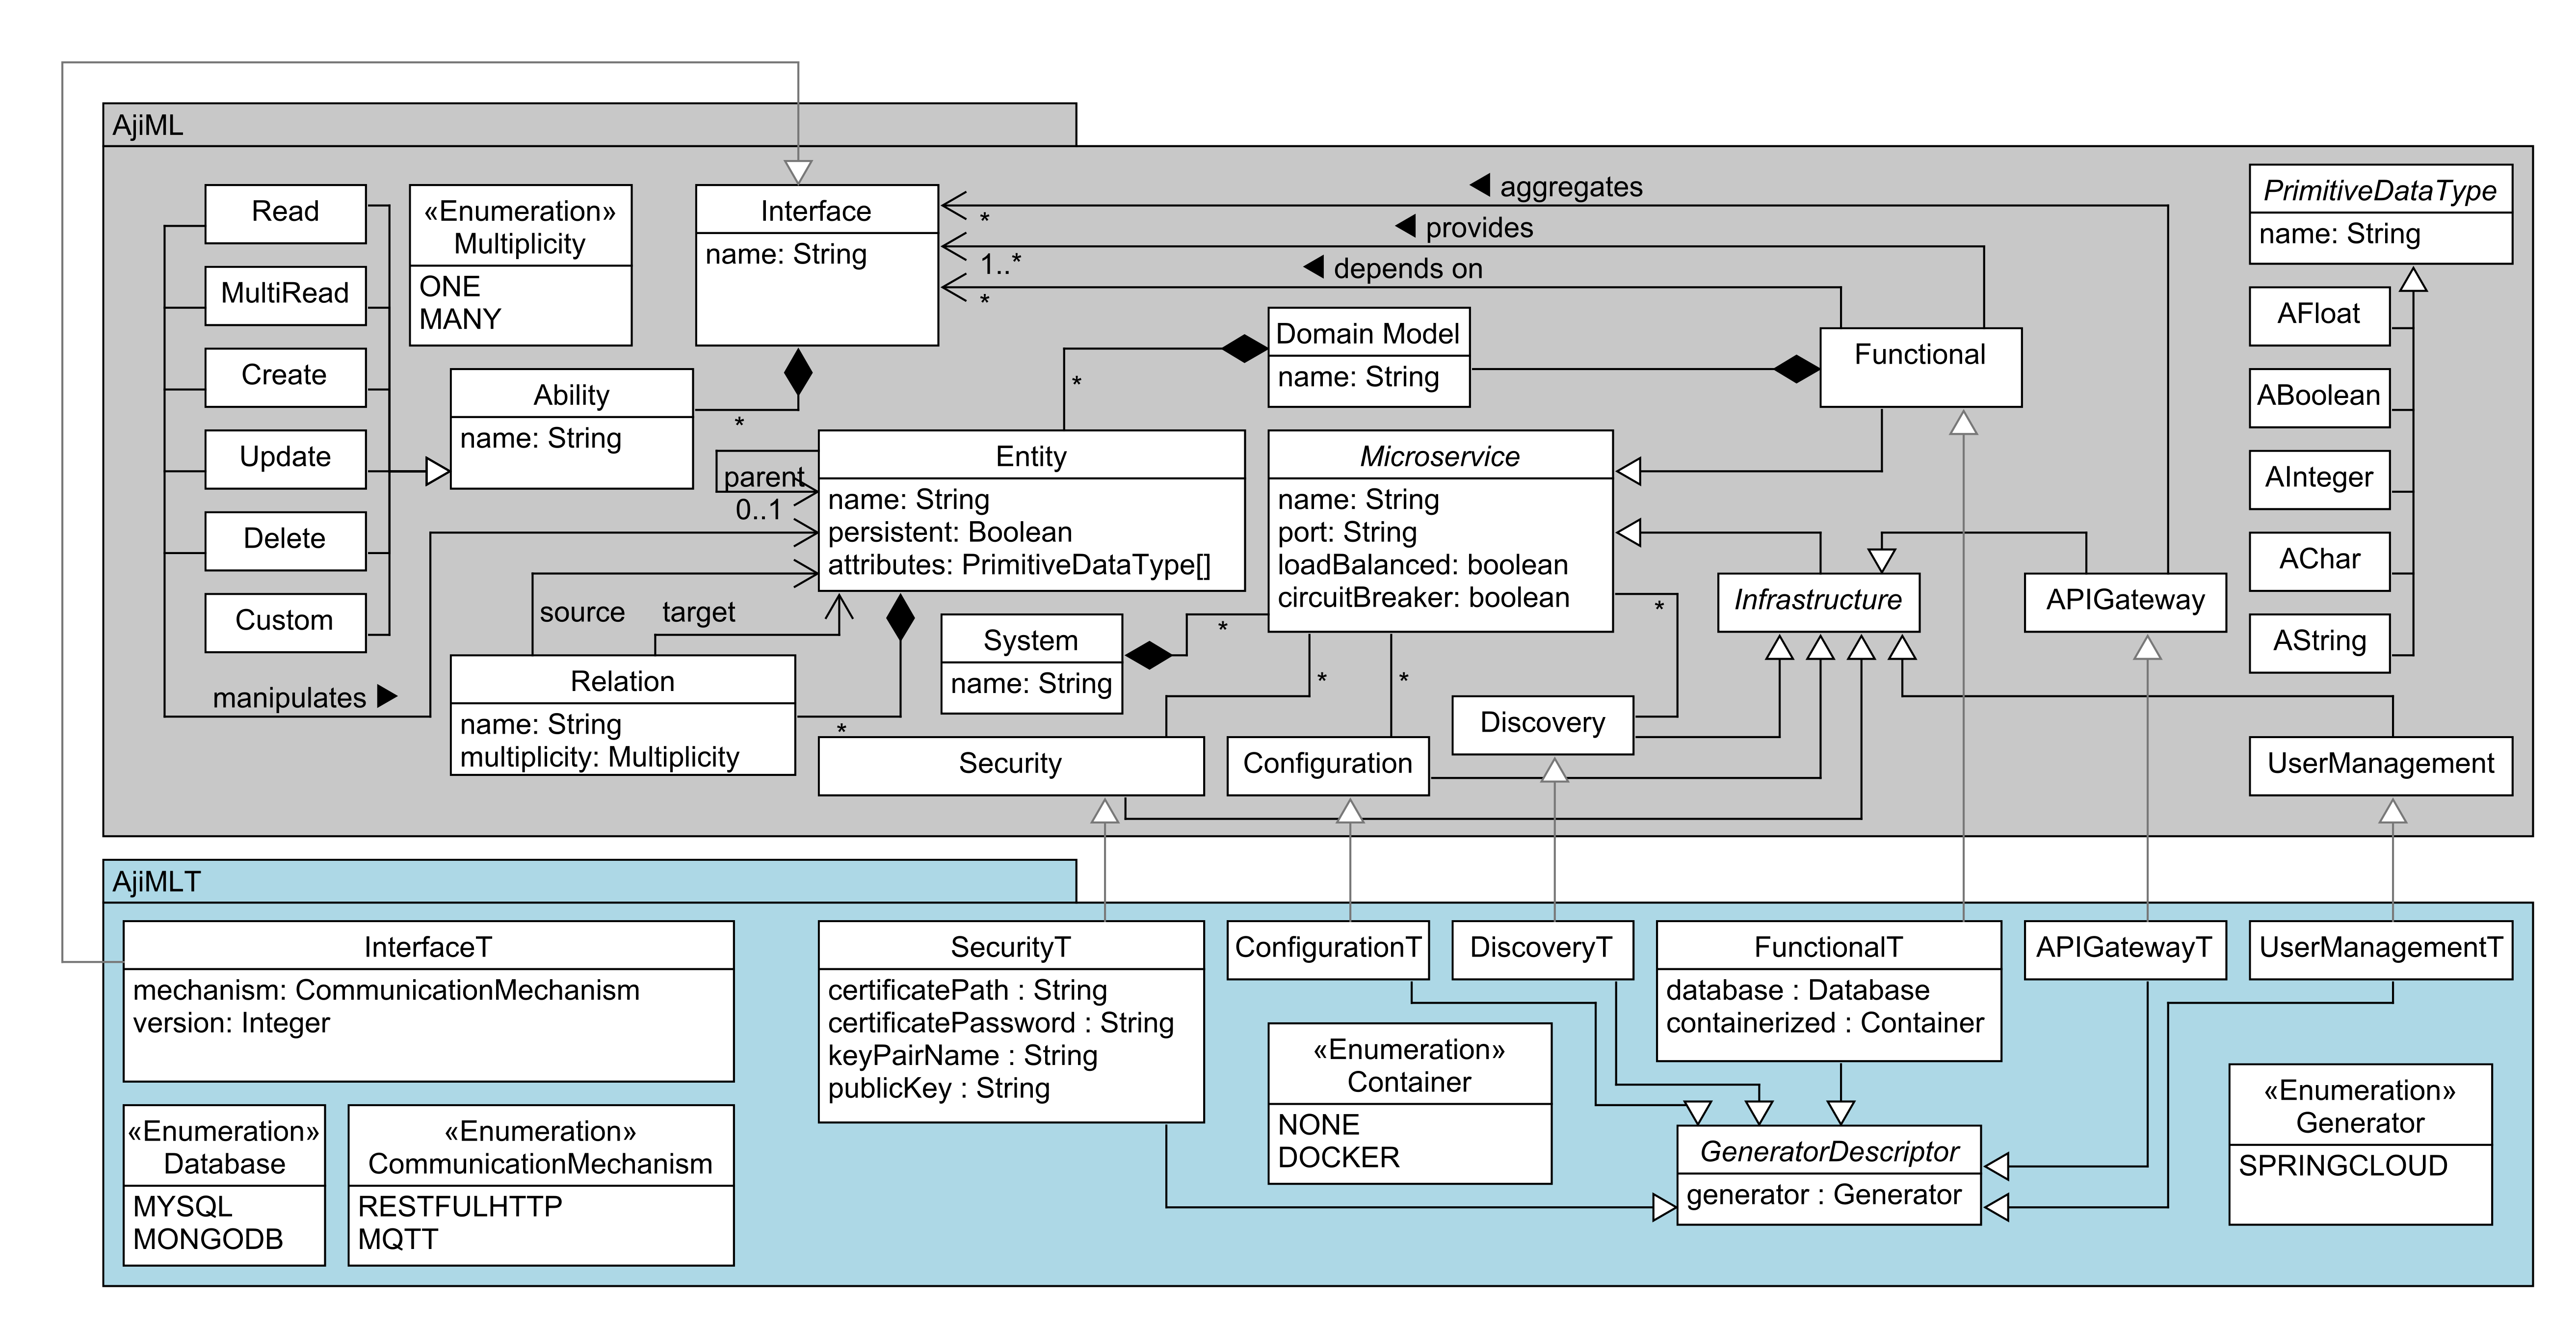
\includegraphics[height=8cm]{bilder/k3/k3_ajil.png}
\captionof{figure}{Metamodell von Ajil}
\end{center}

AjiL bildet in seinem Metamodell verschiedene Aspekte von Microservice-Architekturen ab: So existieren Domain-Modelle und Entitäten, welche Fachlichkeiten abbilden. Klassen wie Microservice, Security, Configuration oder Discovery bilden die technischen Metaklassen ab. Ebenso existiert eine Infrastruktur-Klasse. Das AjiMLT-Paket des Metamodells bildet konkrete Typen ab. So existiert ein spezieller Enum, welcher Docker als Container-Typ definiert, oder ein Enum, welcher die Kommunikation einer Schnittstelle spezifiziert, konkret REST oder das Messaging-Protokoll MQTT. Das AjiL-Metamodell bildet einen recht breiten Bereich der Microservice-Entwicklung ab, jedoch reicht es nicht aus, um die im Kapitel „Grundlagen“ beschriebenen Aspekte abzudecken. AjiL setzt vieles davon implizit in den Generierungstemplates um, ohne explizite Modellklassen.

Auch wenn AjiL einige interessante Ansätze bietet, auf denen man aufbauen kann, wie dessen Ansatz zum Schnittstellenmanagement und der ähnlichen Anforderungen an die zu generierenden Anwendungen, ist AjiL keine hinreichende Lösung, um DDD abzubilden und deploybare Anwendungen zu generieren.

\subsubsection{Context Mapper}

%TODO Quelle angeben
\begin{center}
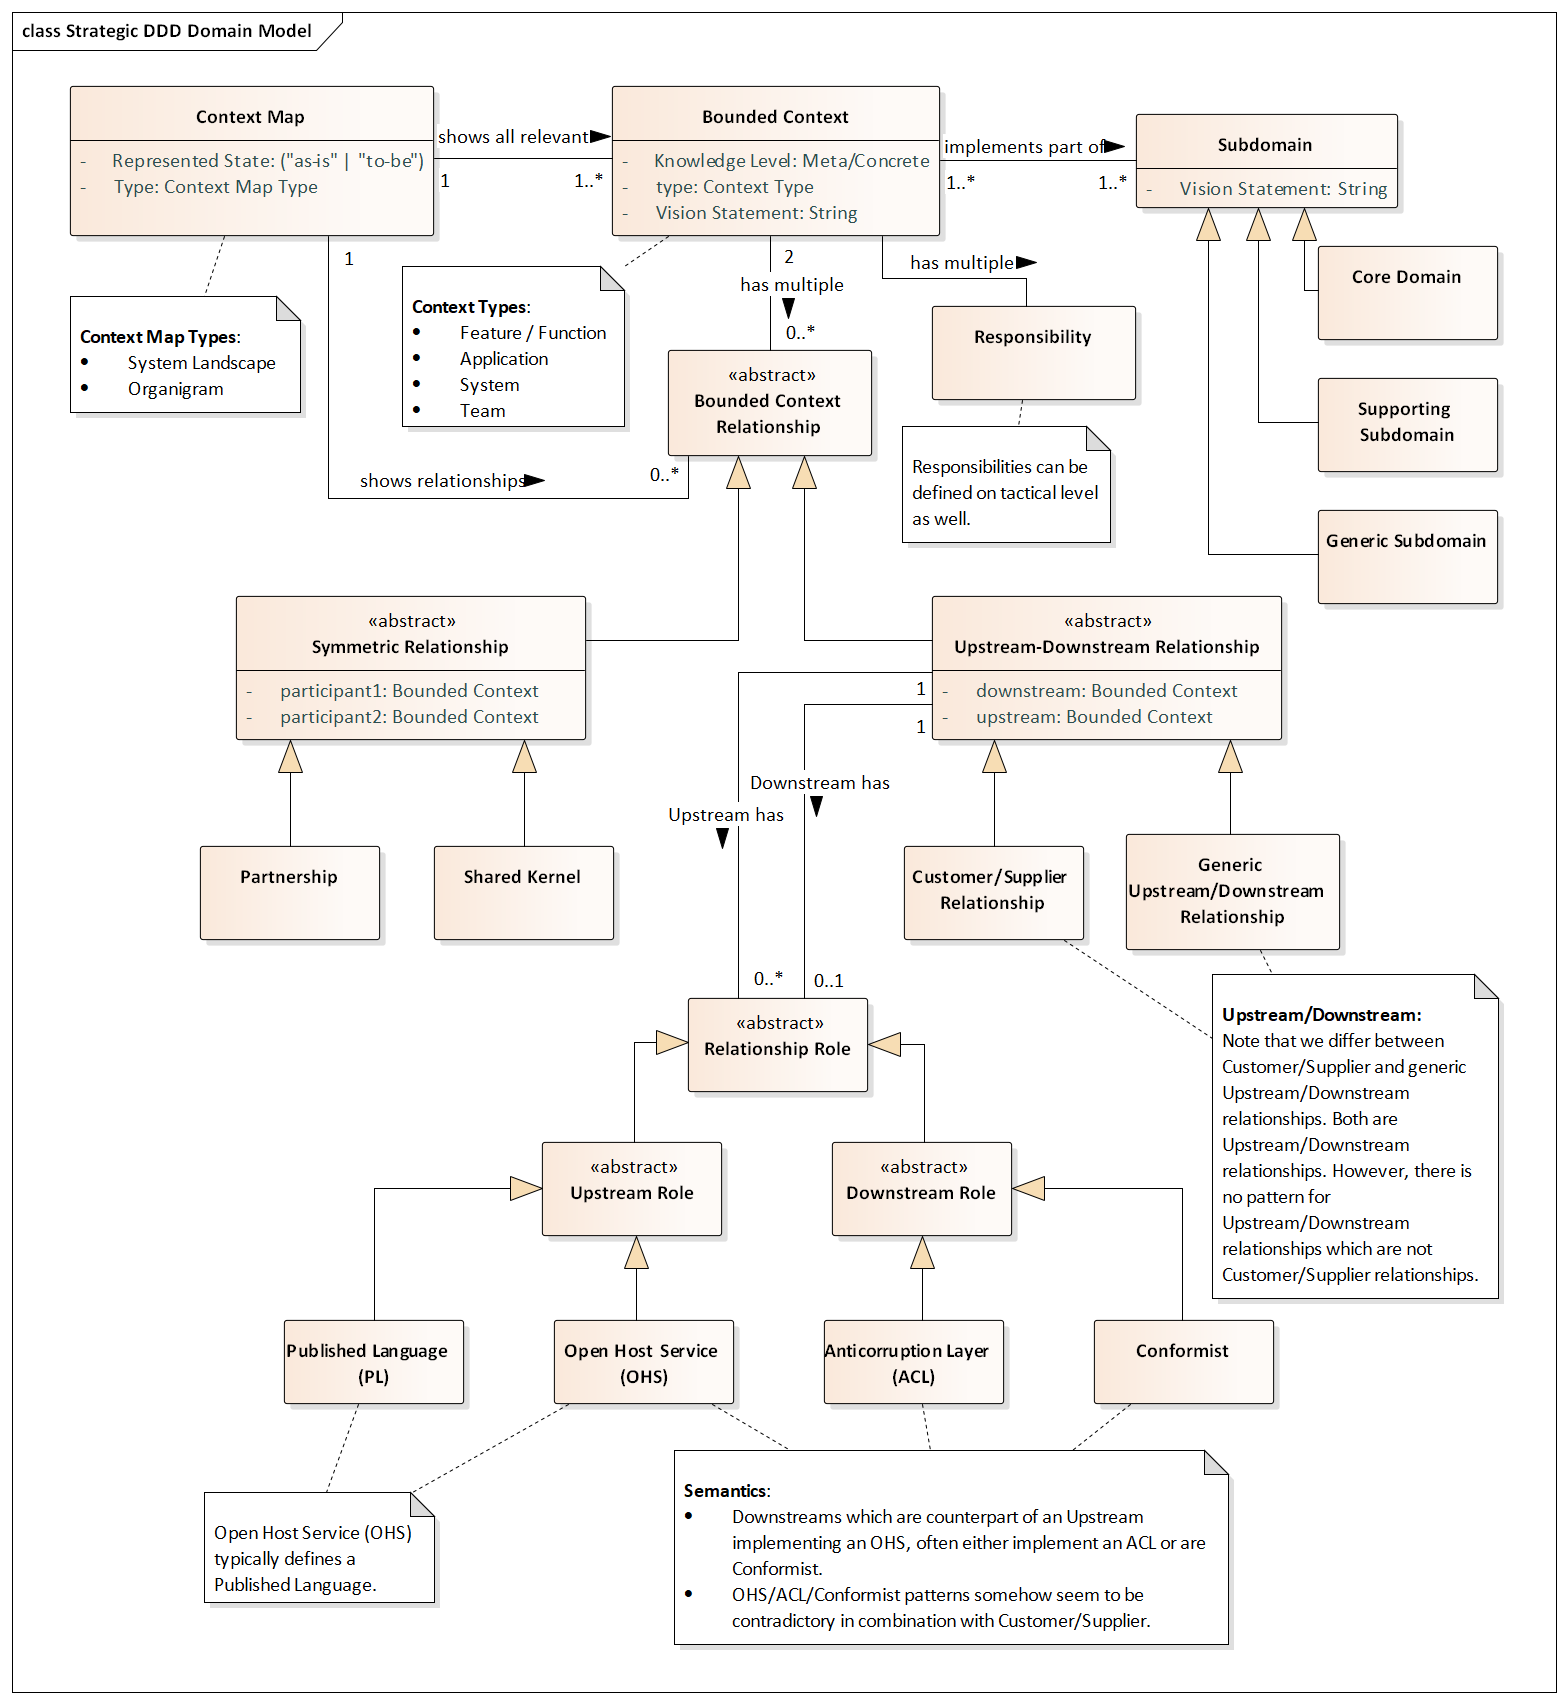
\includegraphics[height=15cm]{bilder/k3/k3_context_mapper.png}
\captionof{figure}{Metamodell von Context Mapper}
\end{center}

Context Mapper definiert ein sehr umfassendes Metamodell, welches die Konzepte des DDD in höchster Ausführlichkeit modelliert. Context Mapper nutzt dieses, um Context Maps von Domänen zu generieren. Dementsprechend ist die Technologie keine Lösung, um Microservice-Anwendungen zu generieren. Jedoch ist die Modellierung eine umfassende Grundlage für eine Metamodellschicht, die das DDD abbildet. Eine exakte Wiederverwendung bietet sich aus Gründen der Übersichtlichkeit nicht an, da Context Mapper eine so umfassende Modellierung ist, dass eine Modellierung mit dem Fokus auf generierende Anwendungen auch mit weniger Metamodell-Klassen auskommen kann. So ist beispielsweise die explizite Modellierung von Responsibilities oder Subdomains für zu generierende Microservices nicht von Belang.

\subsubsection{OCGI}

%TODO Quelle angeben
\begin{center}
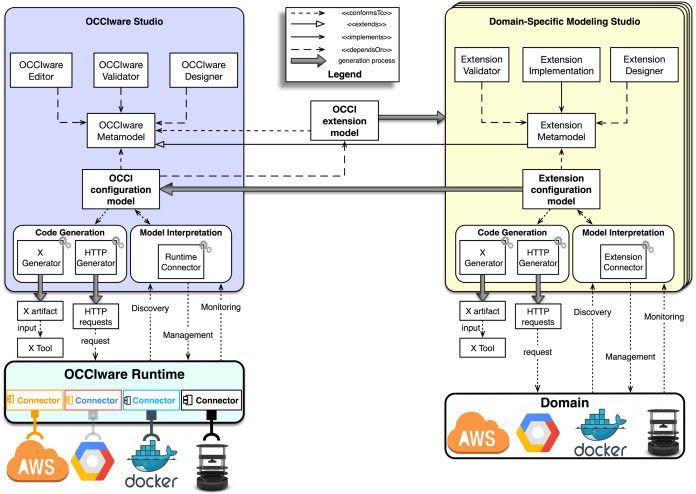
\includegraphics[height=10cm]{bilder/k3/k3_ocgi.jpg}
\captionof{figure}{Metamodell von Ocgi}
\end{center}

\begin{itemize}
\item Erklärung des Metamodells
\item Stärken und Schwächen im Kontext der Zielsetzung
\end{itemize}

\subsubsection{ARGON}

%TODO Quelle angeben
\begin{center}
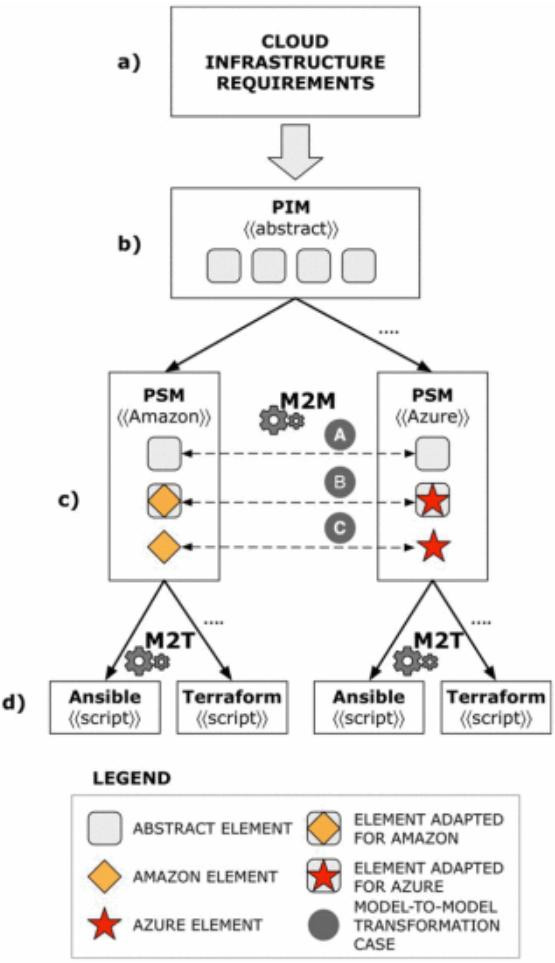
\includegraphics[height=13cm]{bilder/k3/k3_argon.jpg}
\captionof{figure}{Anwendungsschema ARGON}
\end{center}

\begin{itemize}
\item Erklärung des Metamodells
\item Stärken und Schwächen im Kontext der Zielsetzung
\end{itemize}


\subsection{Auswahl der Technologie}

Die Umsetzung des Metamodells erfolgt mit dem Eclipse Modeling Framework (EMF), einem quelloffenen Java-Framework. Weiterhin kommen die ebenfalls quelloffenen Frameworks Eclipse Sirius, das die Visualisierung von Modellen ermöglicht, und Acceleo, das aus EMF-Modellen Code generieren kann, zum Einsatz. Diese stehen Eclipse als Plugins zur Verfügung. Die generierten Anwendungen sollen die Programmiersprache Java verwenden. Zudem wird das Spring Framework eingesetzt, welches die Implementierung verschiedenster Strukturen vereinfacht. Als Technologie zur Umsetzung von eventgetriebener Architektur wird Apache Kafka verwendet. Die generierten Applikationen sollen mittels GitHub versioniert und deployt werden können. Als Cloud-Infrastruktur wird die Google Cloud gewählt, in welcher die Anwendungen auf einem Kubernetes-Cluster laufen sollen.


%%%%%%%%%%%%%%%%%%%%%%%%%%%%%%%%%%%%%%%%%%%%%%%%%%%%%%%%%%%%%%%%%%%%%%%%%%%%%%%%%%%%%%%%%%%%%%%%%%%%%%%%%%%%%%%%%%%%
%			DSL
%%%%%%%%%%%%%%%%%%%%%%%%%%%%%%%%%%%%%%%%%%%%%%%%%%%%%%%%%%%%%%%%%%%%%%%%%%%%%%%%%%%%%%%%%%%%%%%%%%%%%%%%%%%%%%%%%%%%

\section{Entwicklung der eigenen DSL}

\subsubsection{Grundkonzept - Definition verschiedener Modellschichten}

Die Umsetzung des Metamodells erfolgt mit dem Eclipse Modeling Framework (EMF), einem quelloffenen Java-Framework. Weiterhin kommen die ebenfalls quelloffenen Frameworks Eclipse Sirius, das die Visualisierung von Modellen ermöglicht, und Acceleo, das aus EMF-Modellen Code generieren kann, zum Einsatz. Diese stehen als Plugins für Eclipse zur Verfügung. Die generierten Anwendungen sollen die Programmiersprache Java verwenden. Zudem wird das Spring Framework eingesetzt, welches die Implementierung verschiedenster Strukturen vereinfacht. Als Technologie zur Umsetzung von ereignisgetriebener Architektur wird Apache Kafka verwendet. Die generierten Applikationen sollen mittels GitHub versioniert und deployt werden können. Als Cloud-Infrastruktur wird die Google Cloud gewählt, in welcher die Anwendungen auf einem Kubernetes-Cluster laufen sollen.

%TODO Grafik machen
\begin{center}
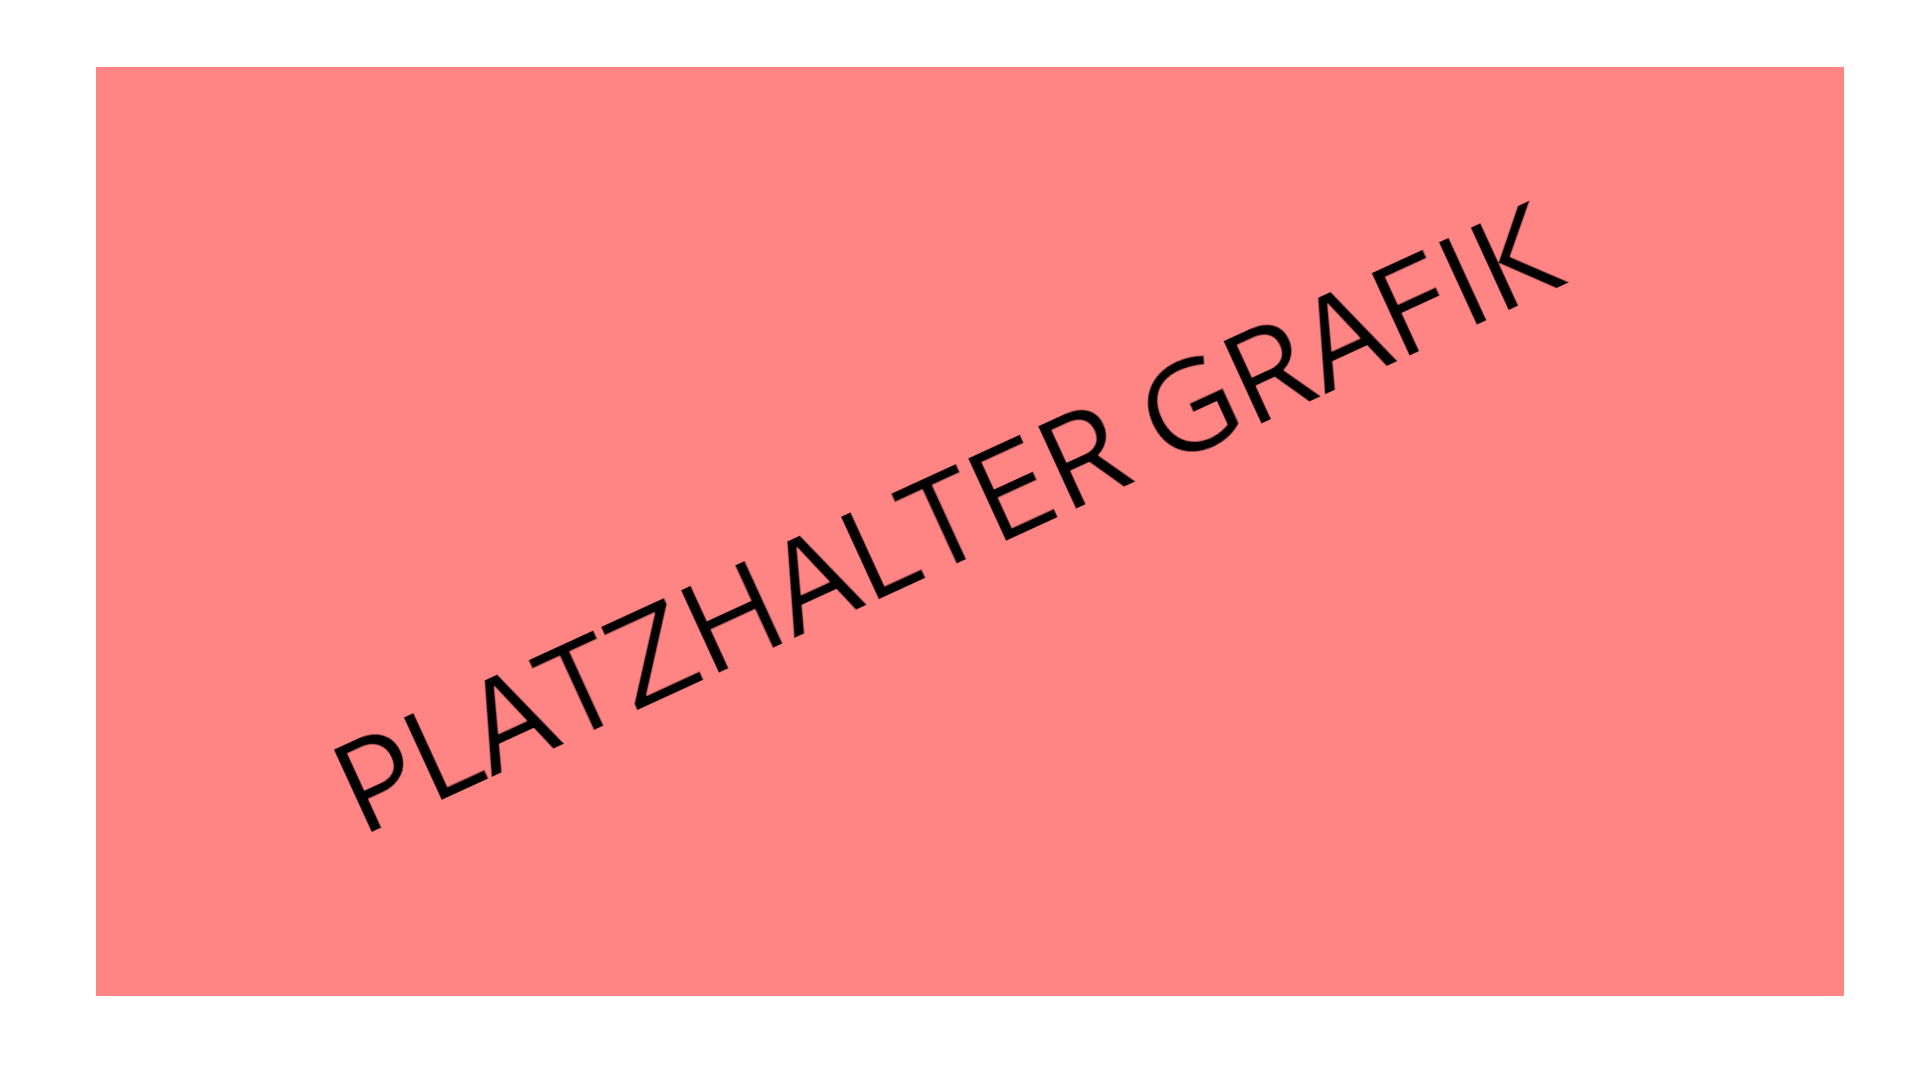
\includegraphics[height=6cm]{bilder/todo.png}
\captionof{figure}{Schichten von Modellen}
\end{center}


%%%%%%%%%%%%%%%%%%%%%%%%%%%%%%%%%%%%%%%%%%%%%%%%%%%%%%%%%%%%%%%%%%%%%%%%%%%%%%%%%%%%%%%%%%%%%%%%%%%%%%%%%%%%%%%%%%%%
%			Fachl. MDD
%%%%%%%%%%%%%%%%%%%%%%%%%%%%%%%%%%%%%%%%%%%%%%%%%%%%%%%%%%%%%%%%%%%%%%%%%%%%%%%%%%%%%%%%%%%%%%%%%%%%%%%%%%%%%%%%%%%%
\subsection{Modellierung der Fachlichkeit}

\subsubsection{Abbildung des MDD in ein Metamodell}

\paragraph{Schicht}

Schichten werden implizit durch das Metamodell vorgegeben.
Nach dem Grundkonzept exisitiert eine fachliche Schicht und eine technische Schicht, welche die Anwendungsschicht bilden. Außerdem existiert eine Infrastrukturschicht und eine Migrationsschicht.
Weiterhin werden Domänenmodelle der fachlichen Schicht werden nach dem DDD auf eine eigene Schicht in der technischen Schicht abgebildet, eier Domänenschicht.

\newpage
\paragraph{Packages}

%TODO Grafik machen
\begin{center}
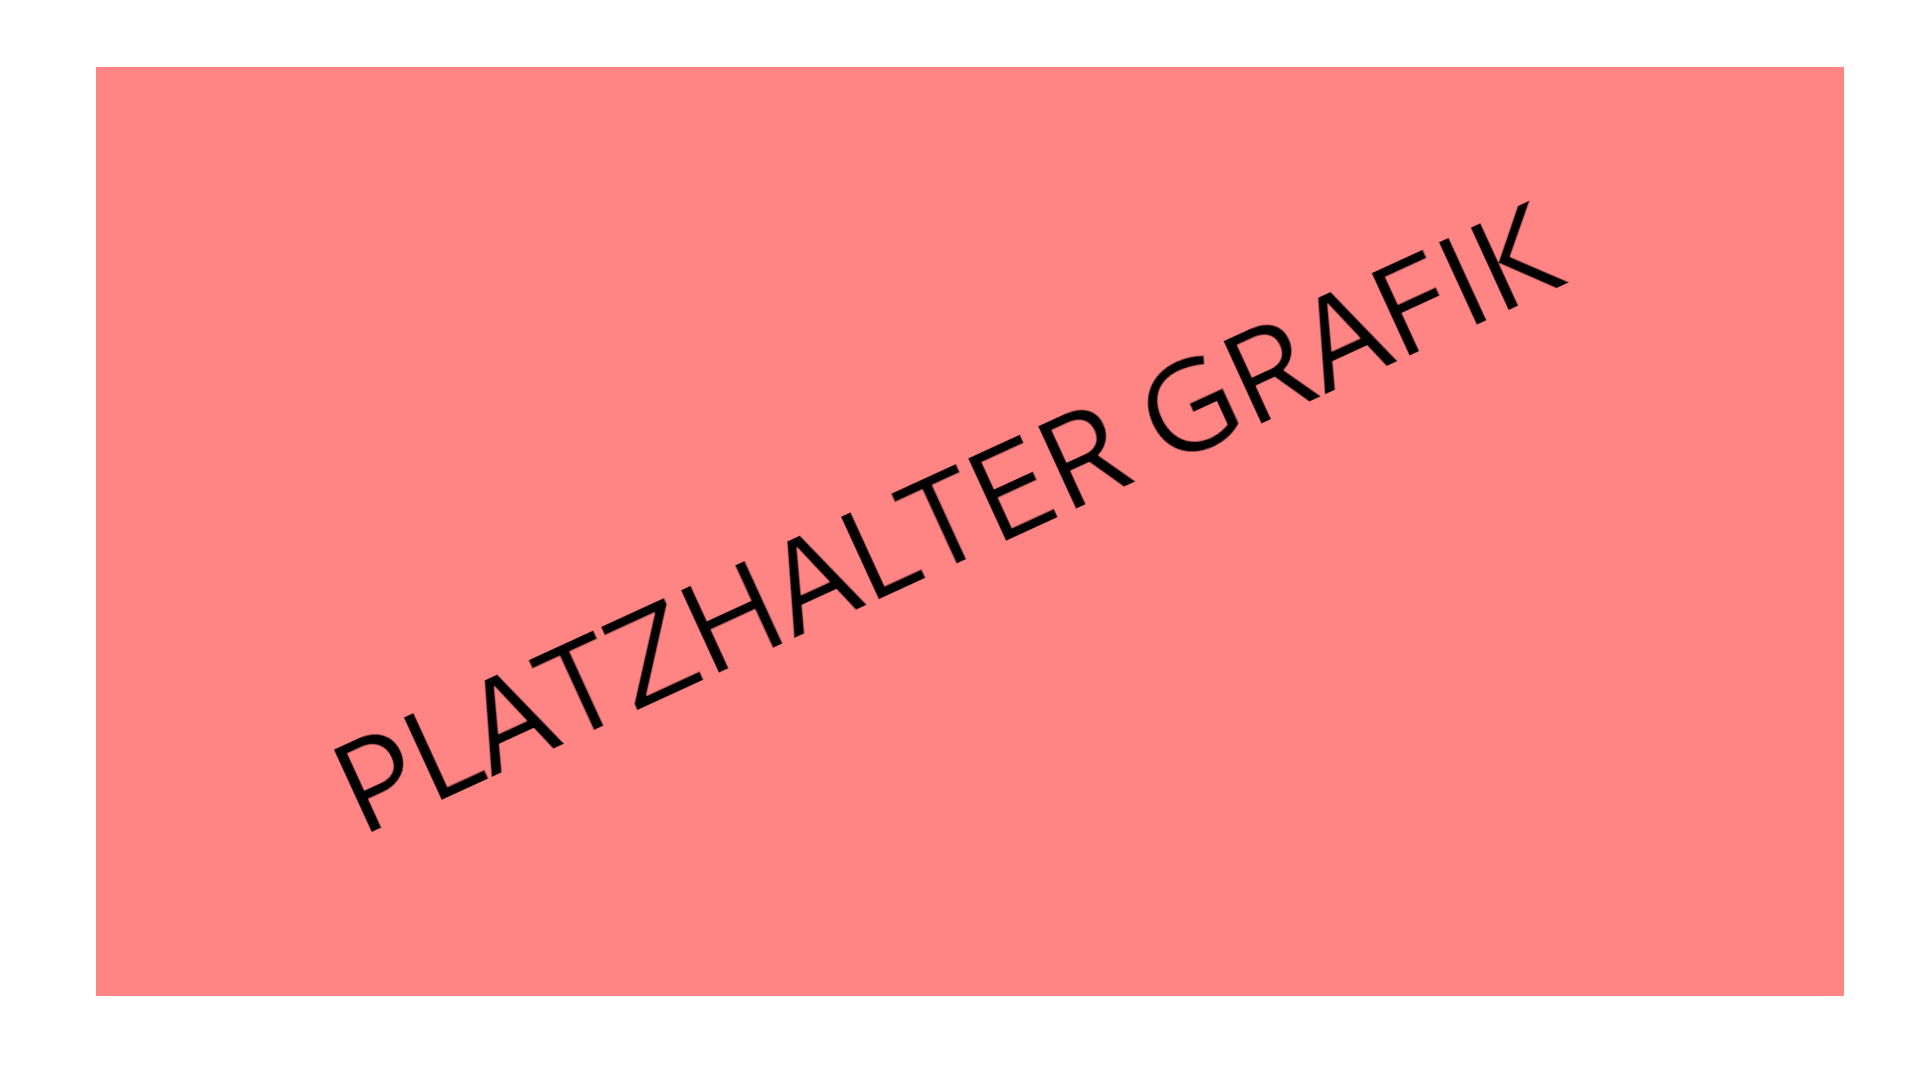
\includegraphics[height=6cm]{bilder/todo.png}
\captionof{figure}{Metamodell - Klassenname}
\end{center}


Ein Paket ist eine Klasse welche beliebige Elemente bündeln kann. Ein Element kann nur in einem Paket erhalten sein. Ein Paket kann auch weitere Pakete erhalten. Daher wird ein Interface Packageable Element eingeführt, sowie eine Klasse Paket welche die Multiplizität definiert.

\paragraph{Entity}

%TODO Grafik machen
\begin{center}
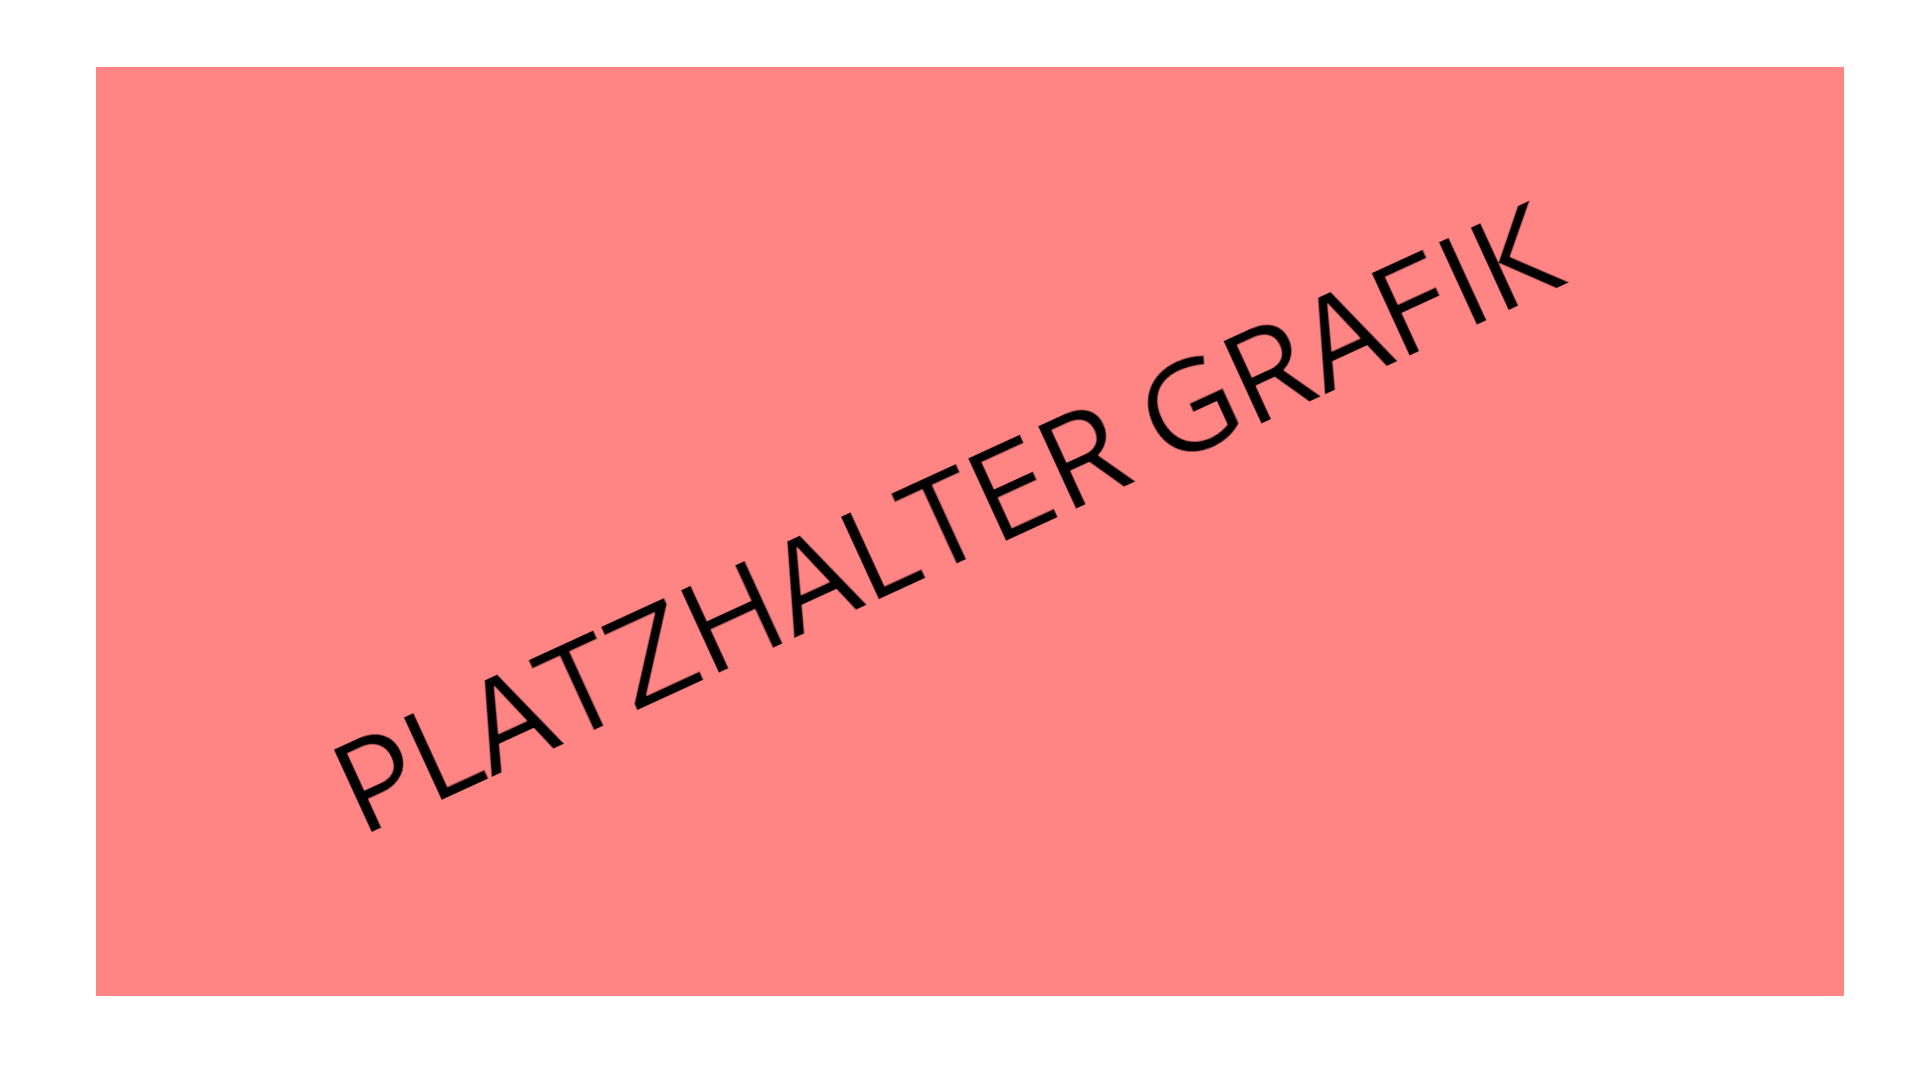
\includegraphics[height=6cm]{bilder/todo.png}
\captionof{figure}{Metamodell - Klassenname}
\end{center}

Entities müssen eine einzigartige ID besitzen um identifizierbar zu sein. Sie können Verhalten besitzen. Entities können Value Objects als Eigenschaften besitzen.

\newpage
\paragraph{Value Object}

%TODO Grafik machen
\begin{center}
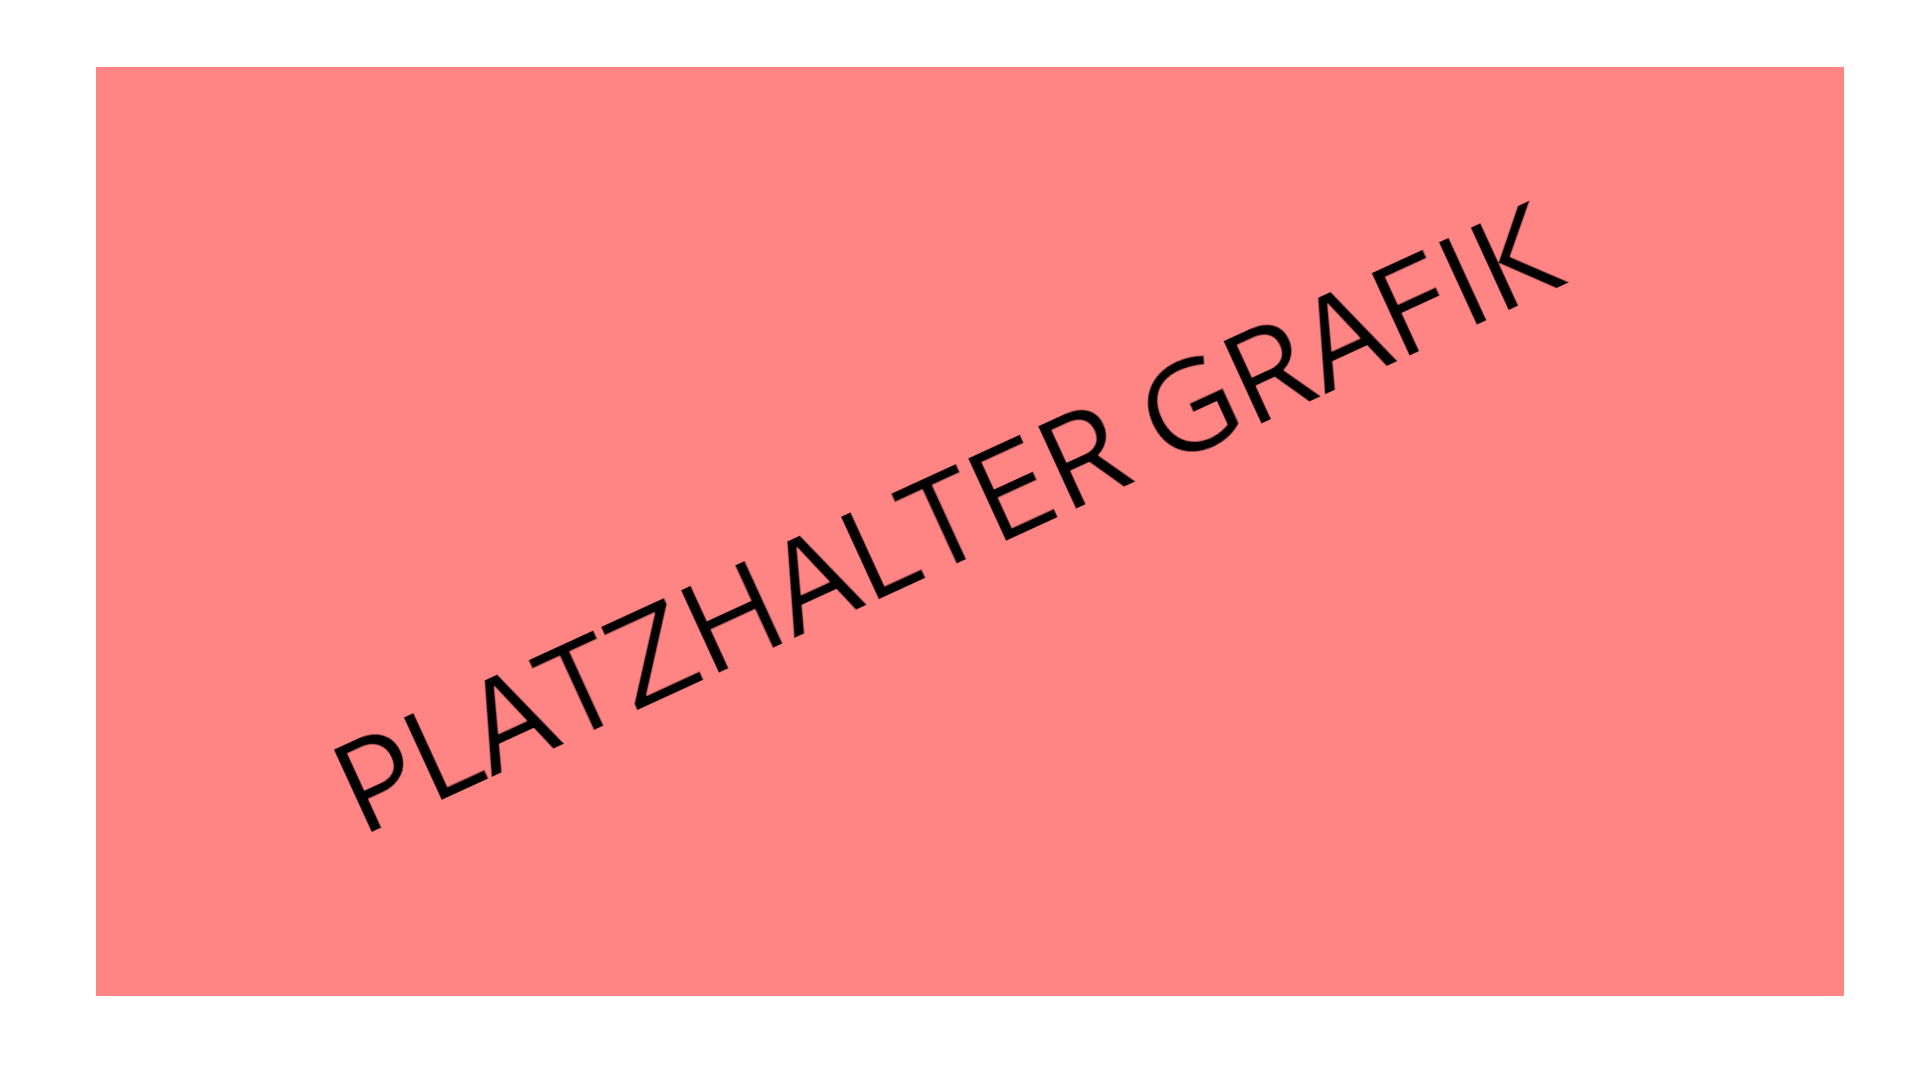
\includegraphics[height=6cm]{bilder/todo.png}
\captionof{figure}{Metamodell - Klassenname}
\end{center}

Value Objects besitzen anderas als Entities keine Identität. Sie können eine Komposition aus anderen Value Objects sein und Entities referenzieren.

\paragraph{Service}

%TODO Grafik machen
\begin{center}
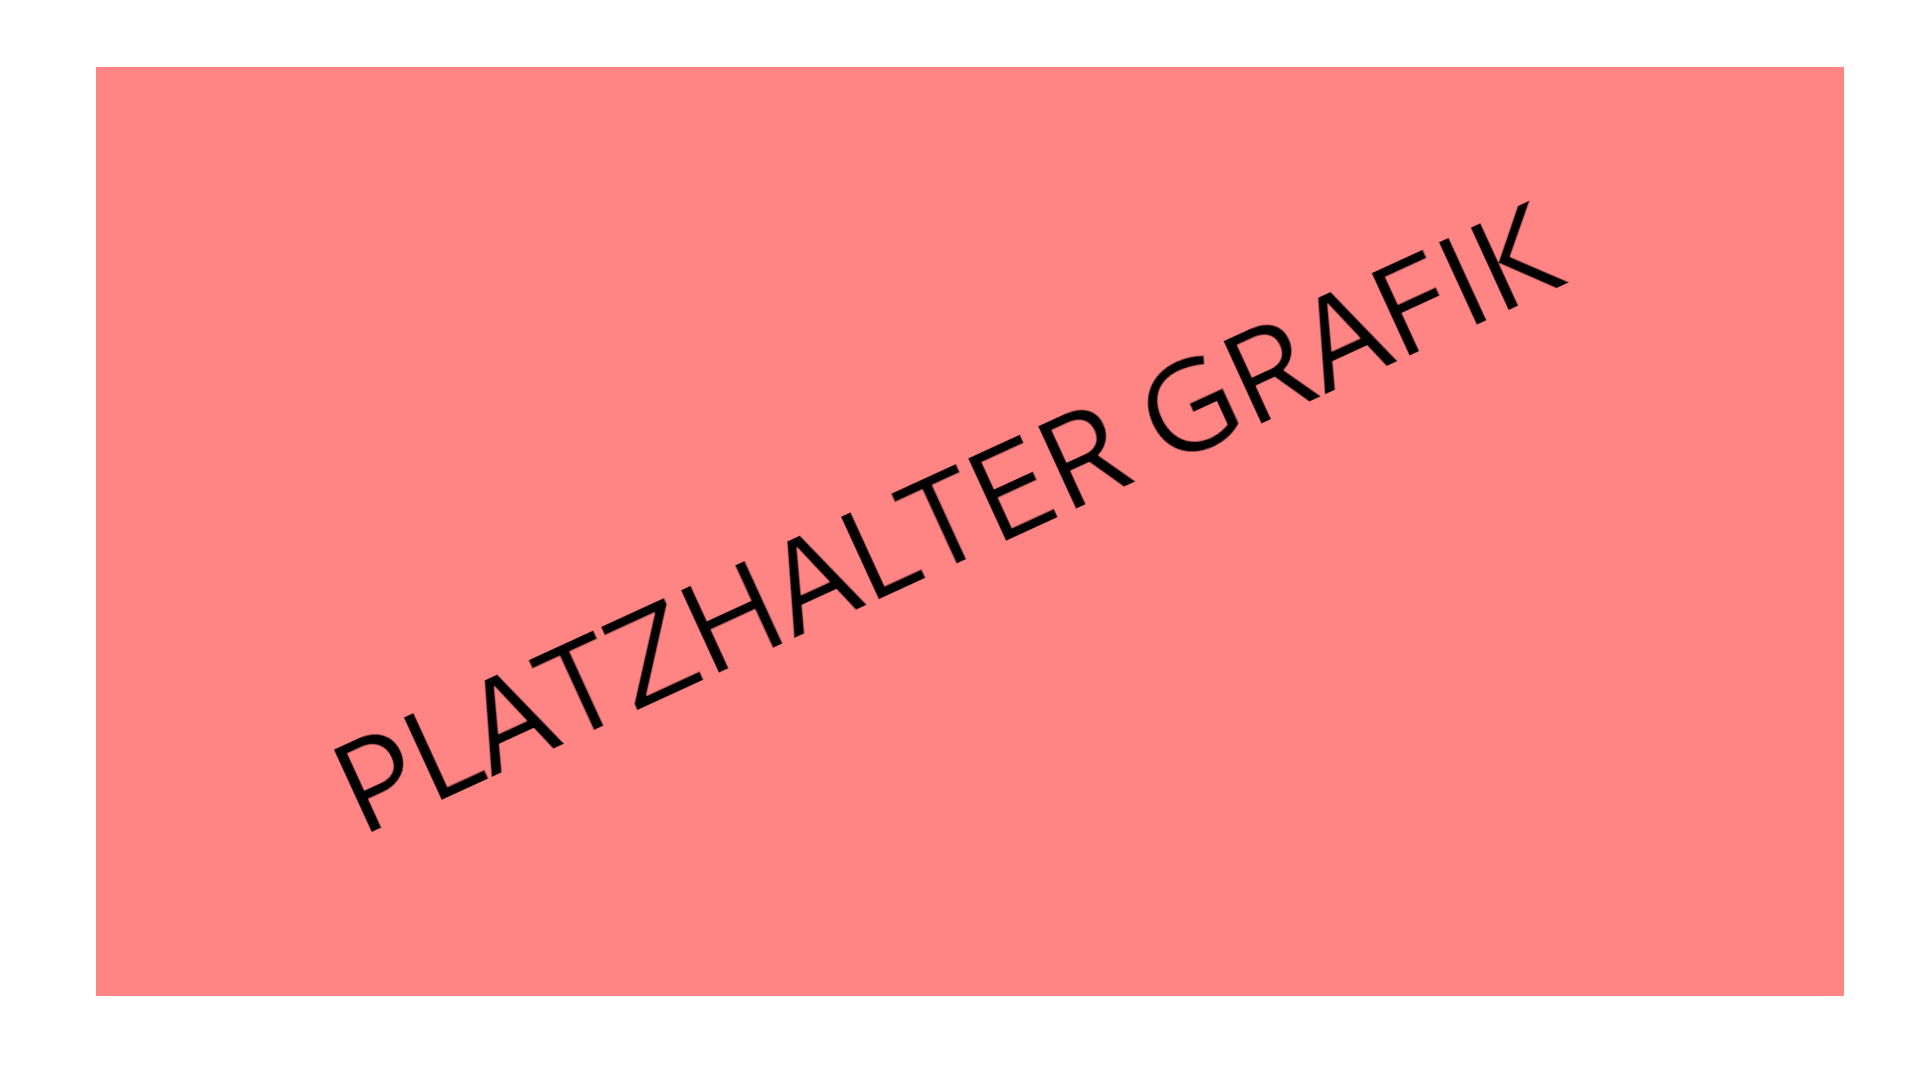
\includegraphics[height=6cm]{bilder/todo.png}
\captionof{figure}{Metamodell - Klassenname}
\end{center}

Services sind Zustsndslose Klassen welche Verhalten umsetzen und nach diesem bennant sind. Sie benötigen eine Schnittstelle zu anderen Elementen des Modells.

\newpage
\paragraph{Aggregate}

%TODO Grafik machen
\begin{center}
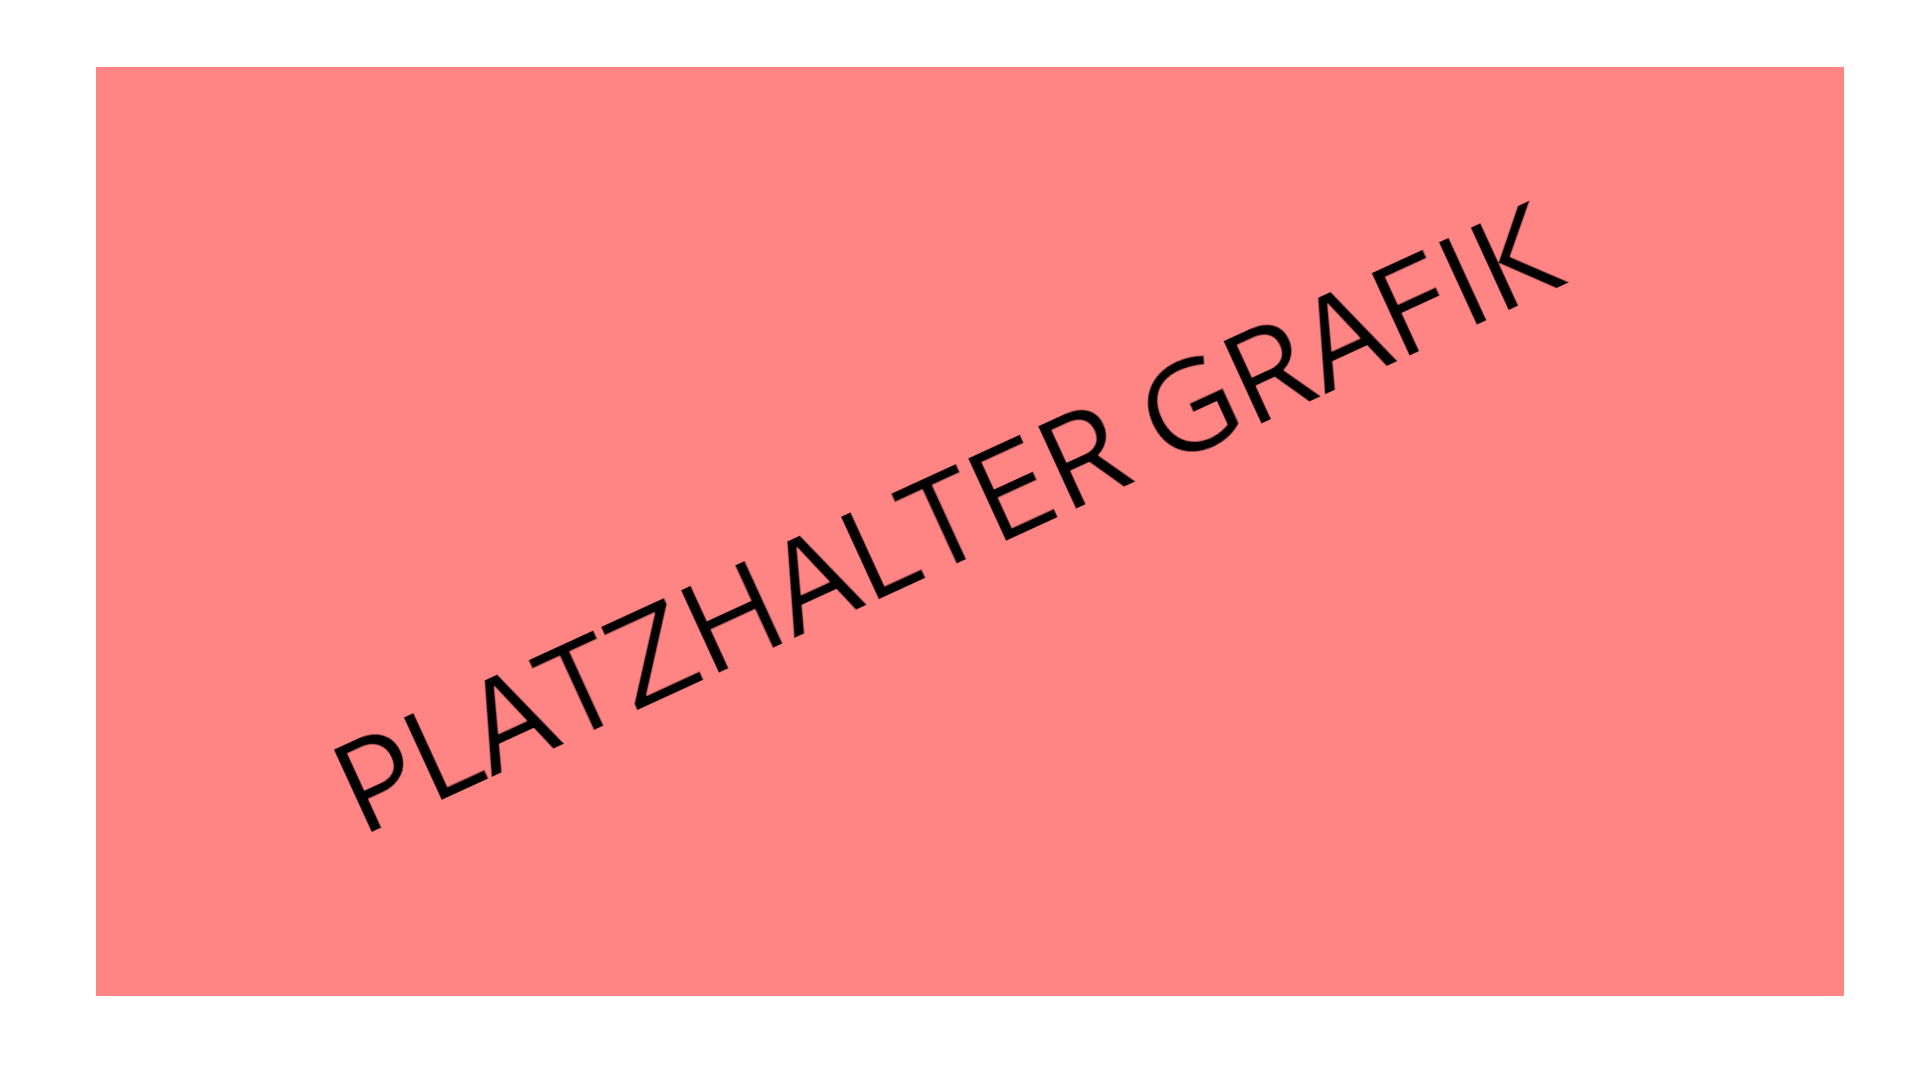
\includegraphics[height=6cm]{bilder/todo.png}
\captionof{figure}{Metamodell - Klassenname}
\end{center}

%TODO Wurzel immer Entität ?
Aggregates bestehen aus einem Wurzelobjekt, einer Entitiy, auf dem andere Objekte verweisen können. Objekte die Teil des Aggregates sind können untereinander auf isch verweisen.

\paragraph{Factory}

%TODO Grafik machen
\begin{center}
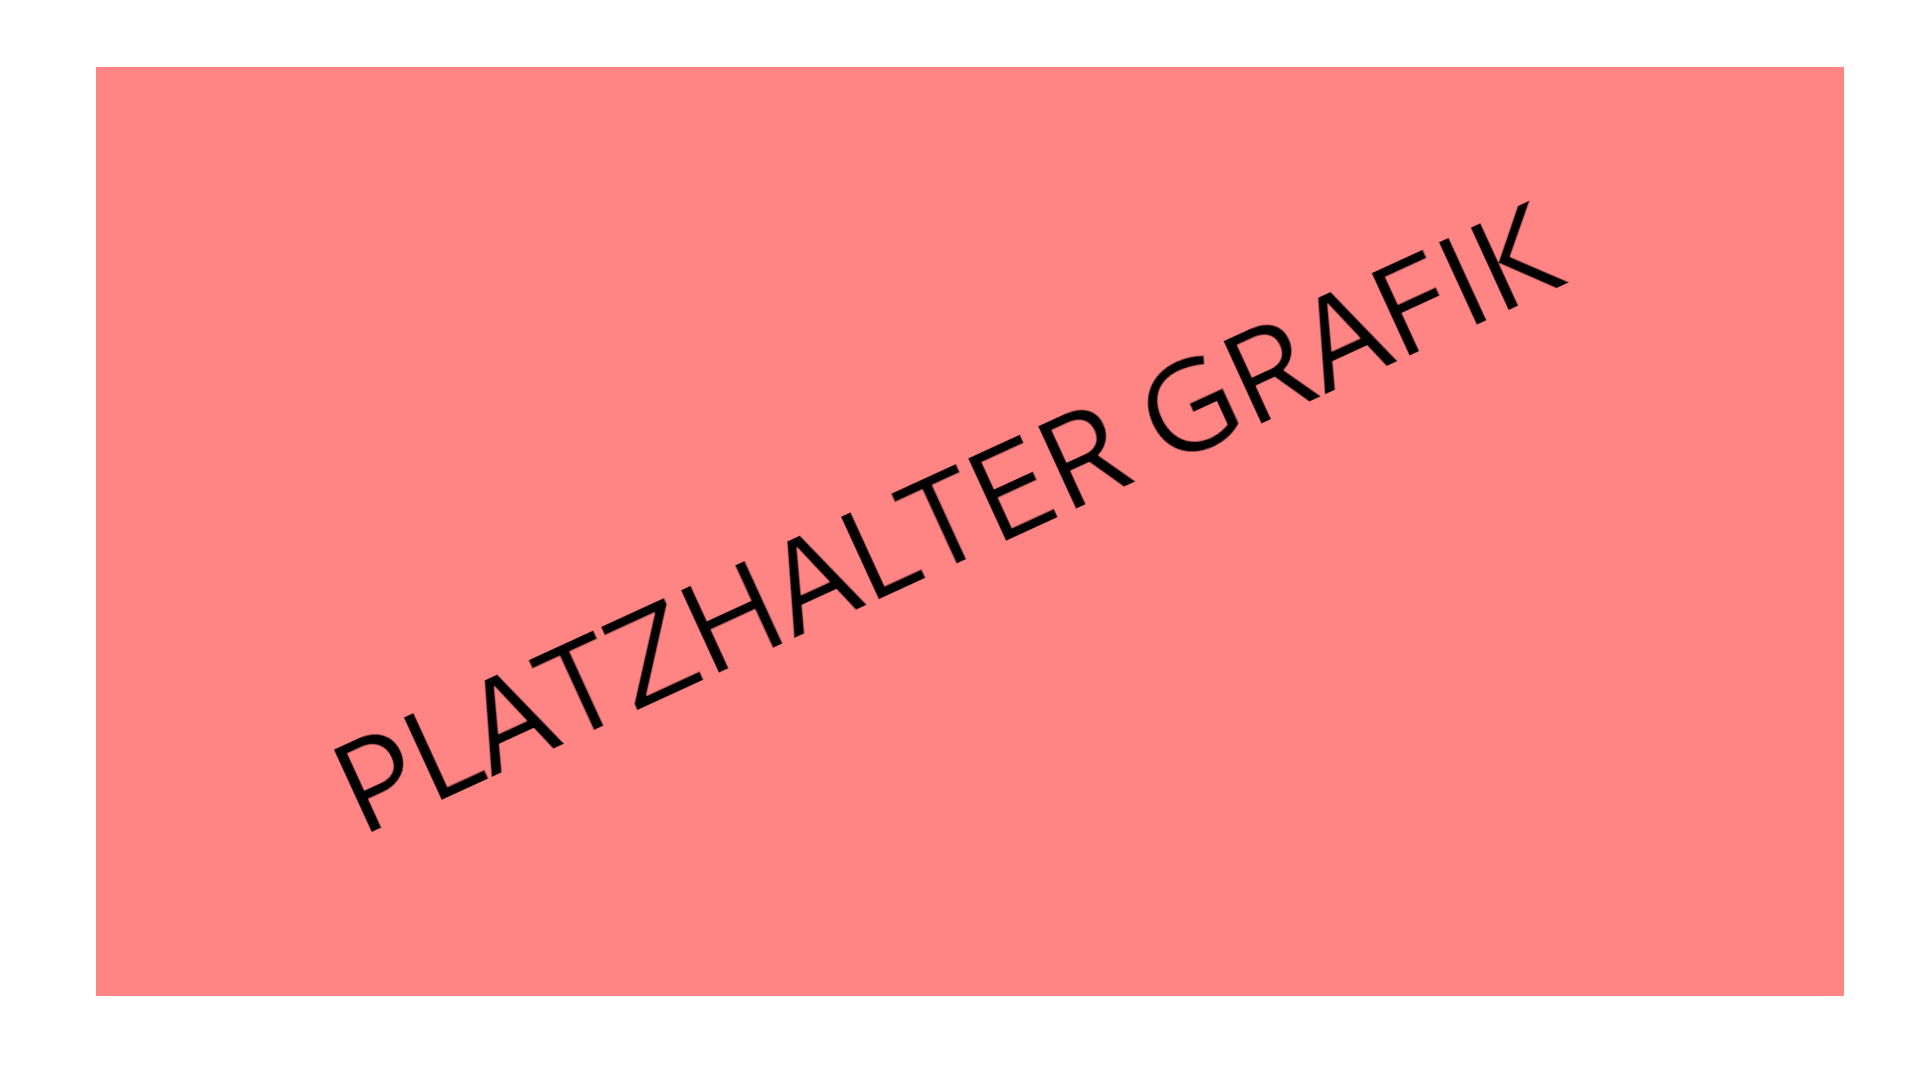
\includegraphics[height=6cm]{bilder/todo.png}
\captionof{figure}{Metamodell - Klassenname}
\end{center}

Factories erstellen Objekte einer Klasse. Dies wird mit einer eindeutigen 1 zu 1 Multiplizität ausgedrückt. Sie besitzt Invarianten die bei der Erstellung geprüft werden müssen. Die Überprüfung kann aber auch auselagert werden. Auch die Wiedererzeugung muss möglich sein.

\newpage
\paragraph{Repository}

%TODO Grafik machen
\begin{center}
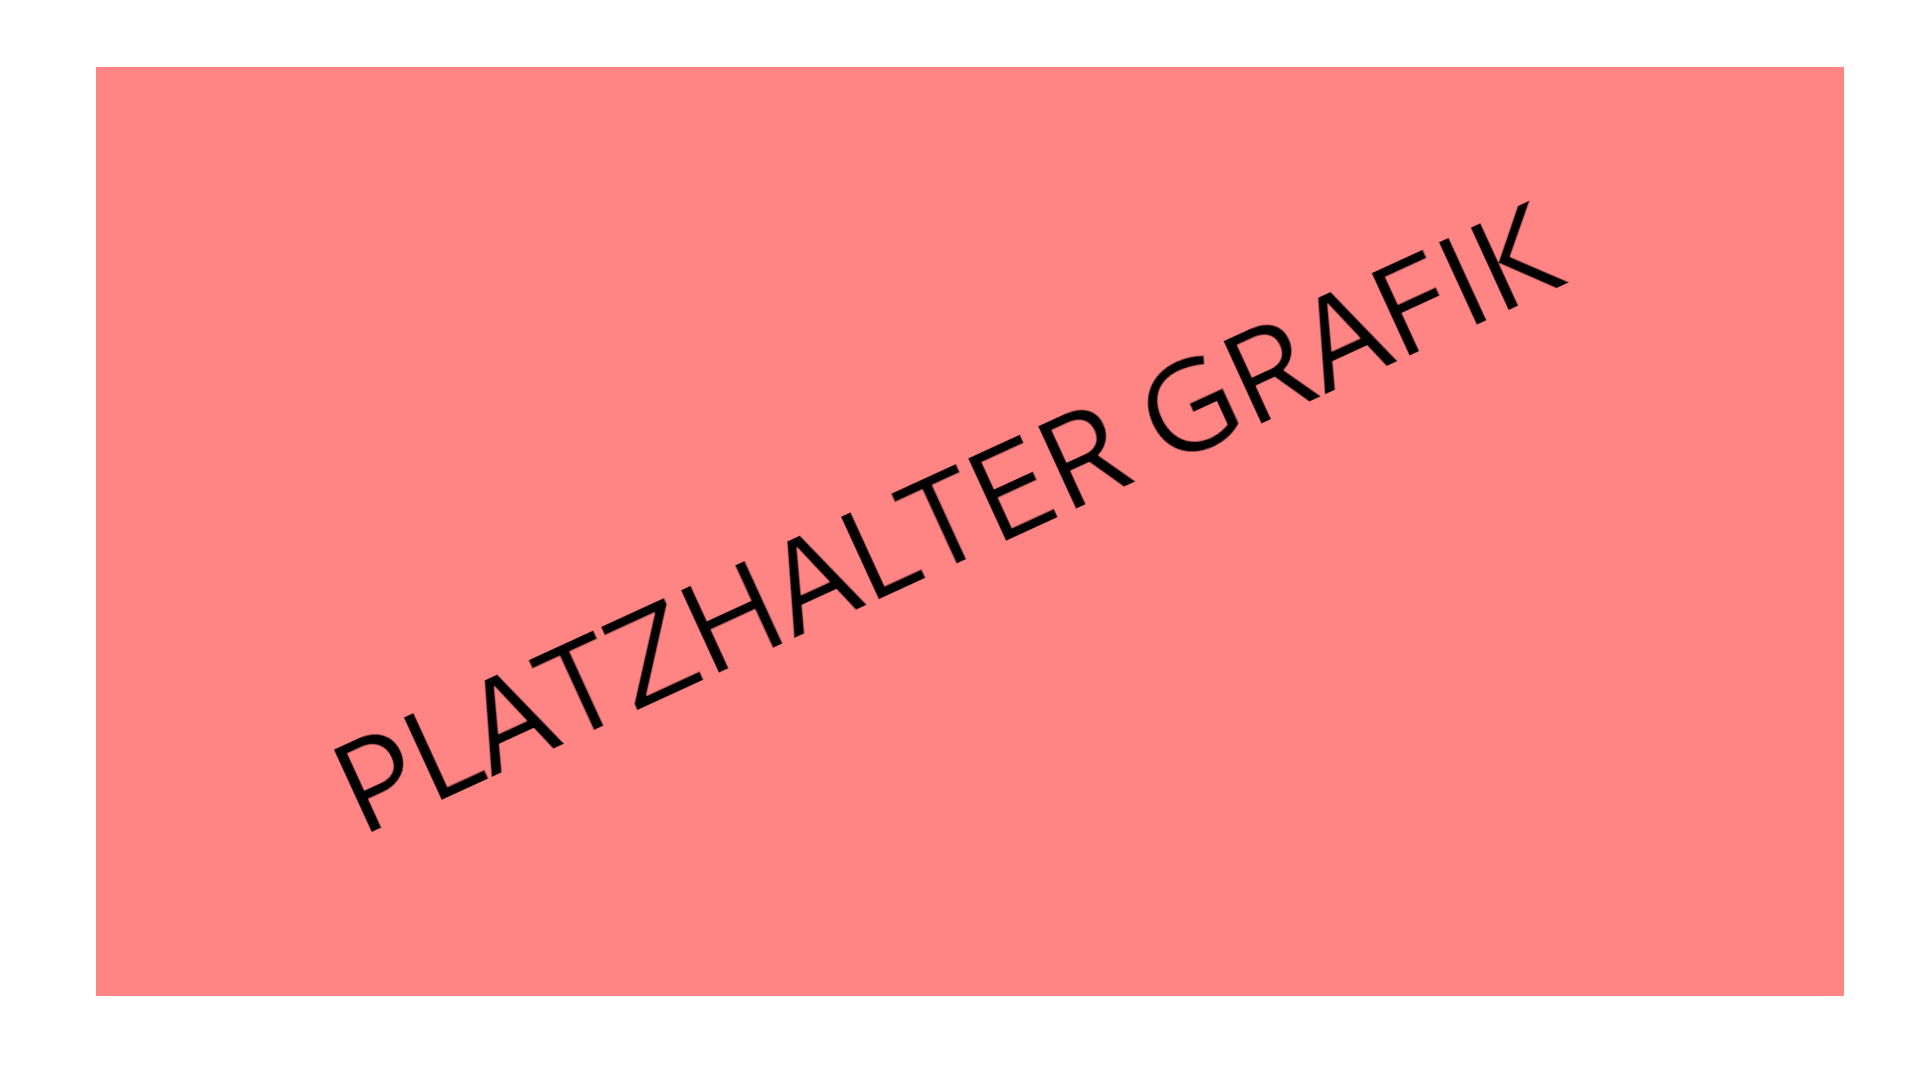
\includegraphics[height=6cm]{bilder/todo.png}
\captionof{figure}{Metamodell - Klassenname}
\end{center}

Repostorys speichern Daten für einen bestimmten Objekttypen, daher 1 zu 1. Mit einer Suche können Objekte aus einem Repository abgefragt werden.

\paragraph{Gesamtüberblick}

\begin{center}
\rotatebox{90}{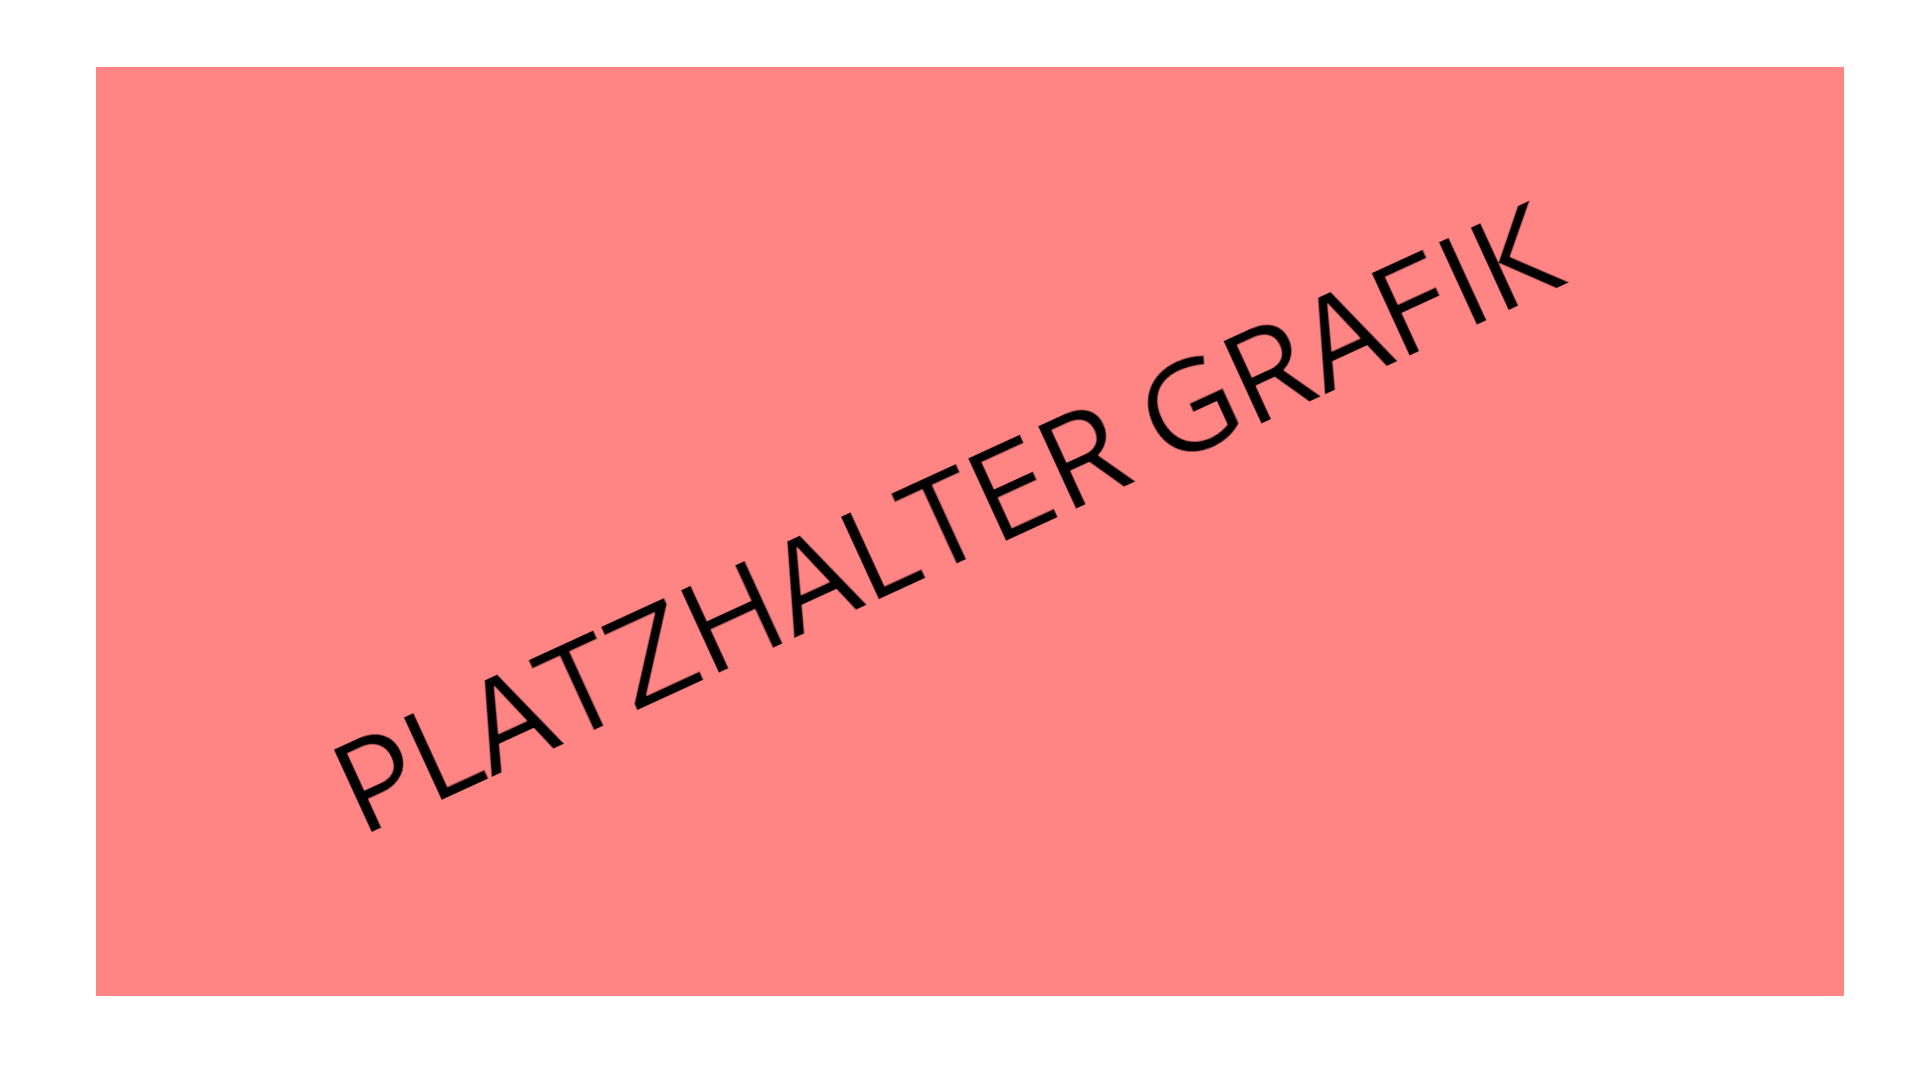
\includegraphics[height=10cm]{bilder/todo.png}}
\captionof{figure}{Metamodell - Klassenname}
\end{center}

%%%%%%%%%%%%%%%%%%%%%%%%%%%%%%%%%%%%%%%%%%%%%%%%%%%%%%%%%%%%%%%%%%%%%%%%%%%%%%%%%%%%%%%%%%%%%%%%%%%%%%%%%%%%%%%%%%%%
%			Fachl. Strategic Design
%%%%%%%%%%%%%%%%%%%%%%%%%%%%%%%%%%%%%%%%%%%%%%%%%%%%%%%%%%%%%%%%%%%%%%%%%%%%%%%%%%%%%%%%%%%%%%%%%%%%%%%%%%%%%%%%%%%%
\newpage
\subsubsection{Abbildung des Strategic Design in ein Metamodell}

\paragraph{Bounded Context}

%TODO Grafik machen
\begin{center}
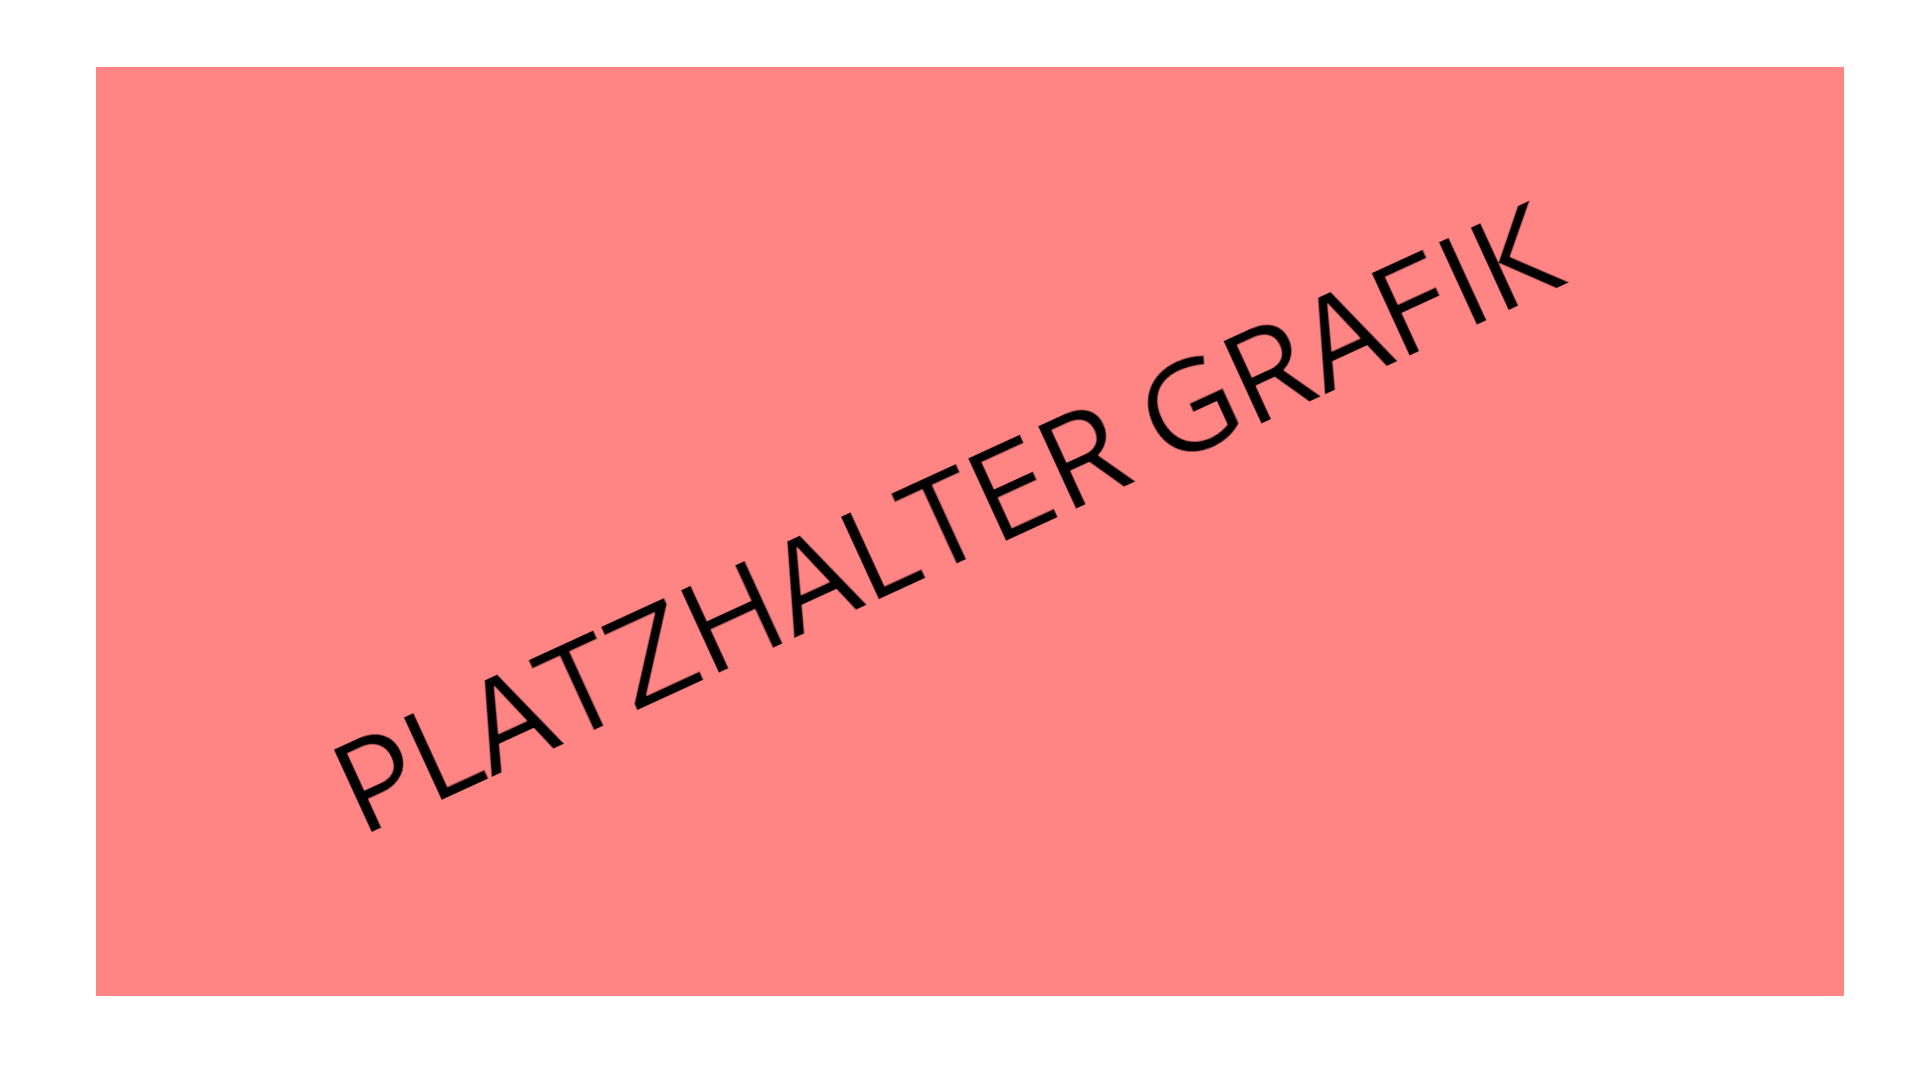
\includegraphics[height=6cm]{bilder/todo.png}
\captionof{figure}{Metamodell - Klassenname}
\end{center}

Ein Bounded Context weißt einem Domänenmodell einen klar definierten Rahmen zu, ist daher also eine gemeinsamer Vaterknoten aller einem Domänenmodell zugehörigen Objekte. Eine abgebildete Domäne wiederum kann aus mehreren solcher Kontexte bestehen. Daher wird dies mit 1 n modelliert. Sie besitzen eine Schnittstelle, welche bestimmt welche Modelle für andere Kontexte verfügbar sind. Sie haben Beziehungen untereinander welche Klassen des Types BoundedContextRelationship sind

\paragraph{Shared Kernel}

%TODO Grafik machen
\begin{center}
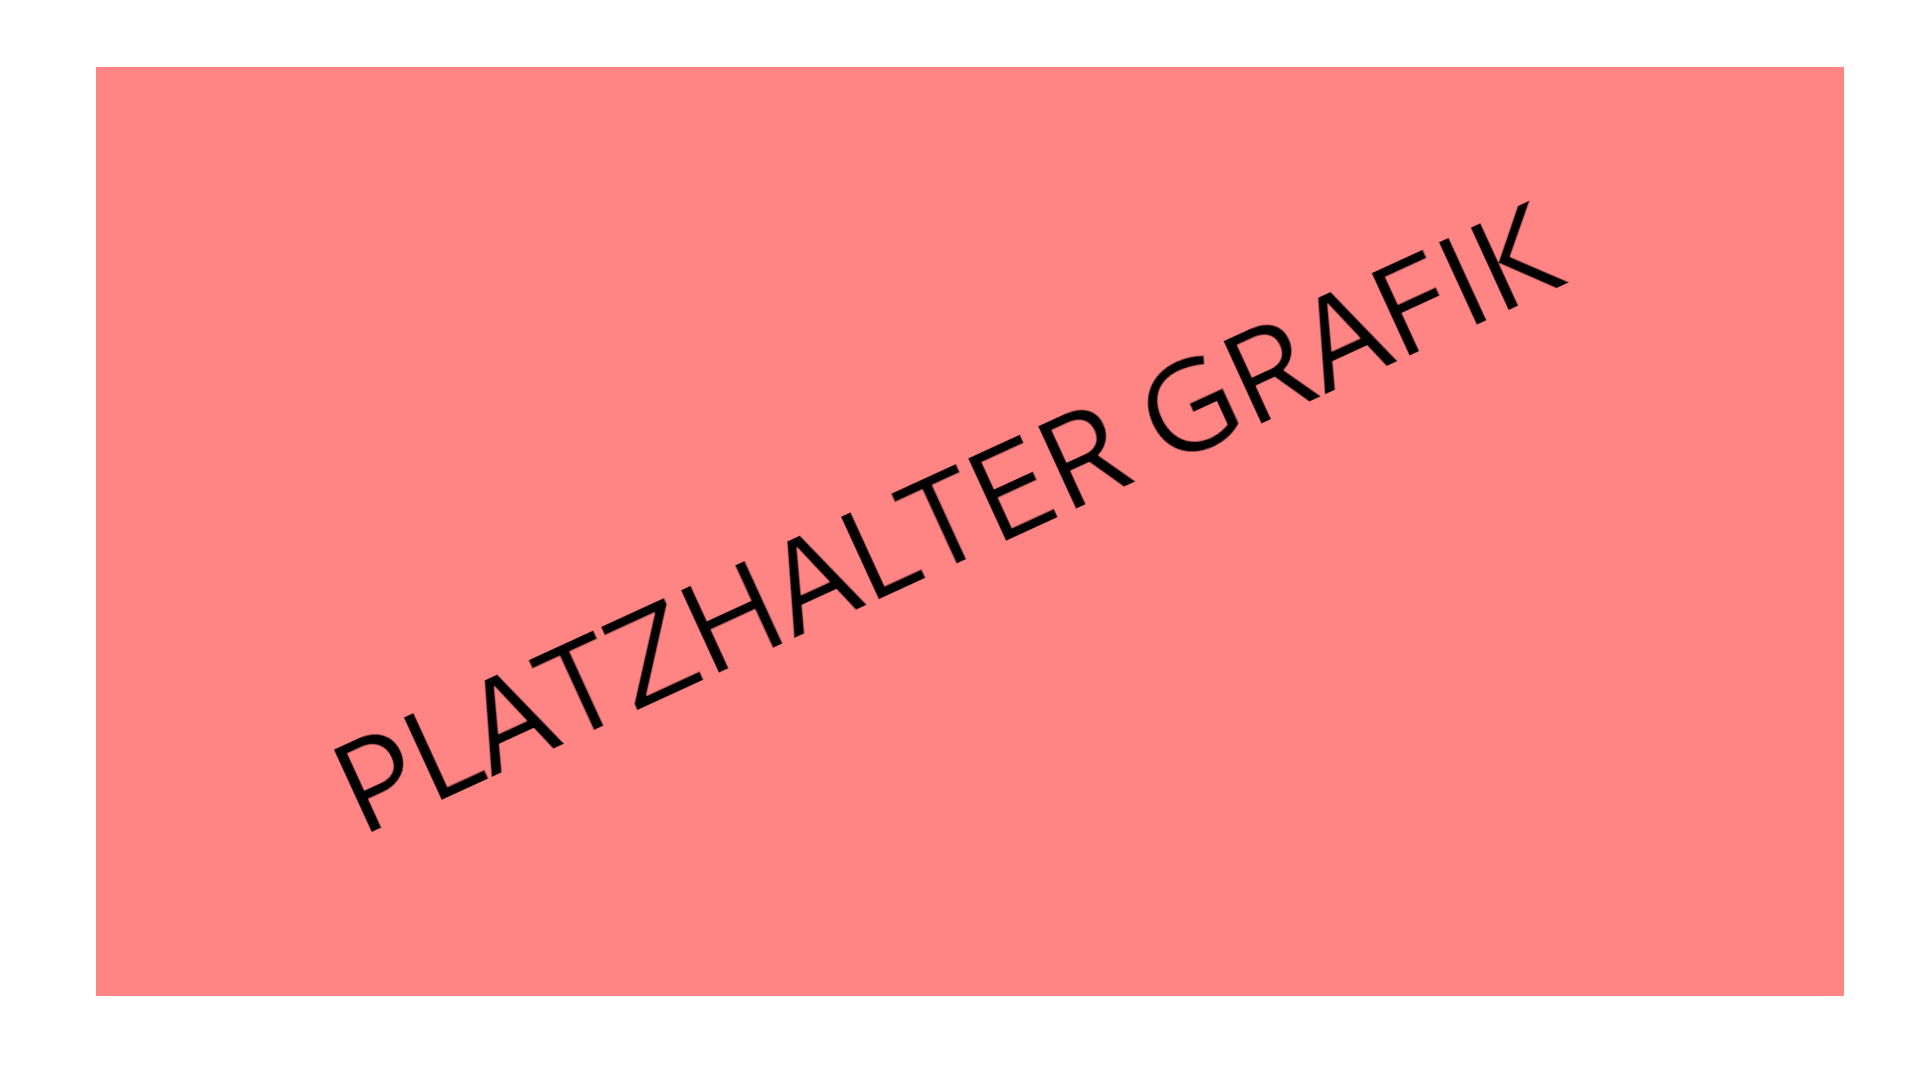
\includegraphics[height=6cm]{bilder/todo.png}
\captionof{figure}{Metamodell - Klassenname}
\end{center}

Weiterhin können Domänenmodelle geteilt werden um in anderen Domännenmodellen mitgenutzt zu werden. Diese Shared Kernel werden als Beziehung unter Domänenmodellen abgebildet. Shared Kernel ist eine optionale Eigenschaft die ein Domänenmodell haben kann. Wenn es diese hat kann es mehrere Domänenmodeller referenzieren, sonst nicht.

\newpage
\paragraph{Customer/Supplier}

%TODO Grafik machen
\begin{center}
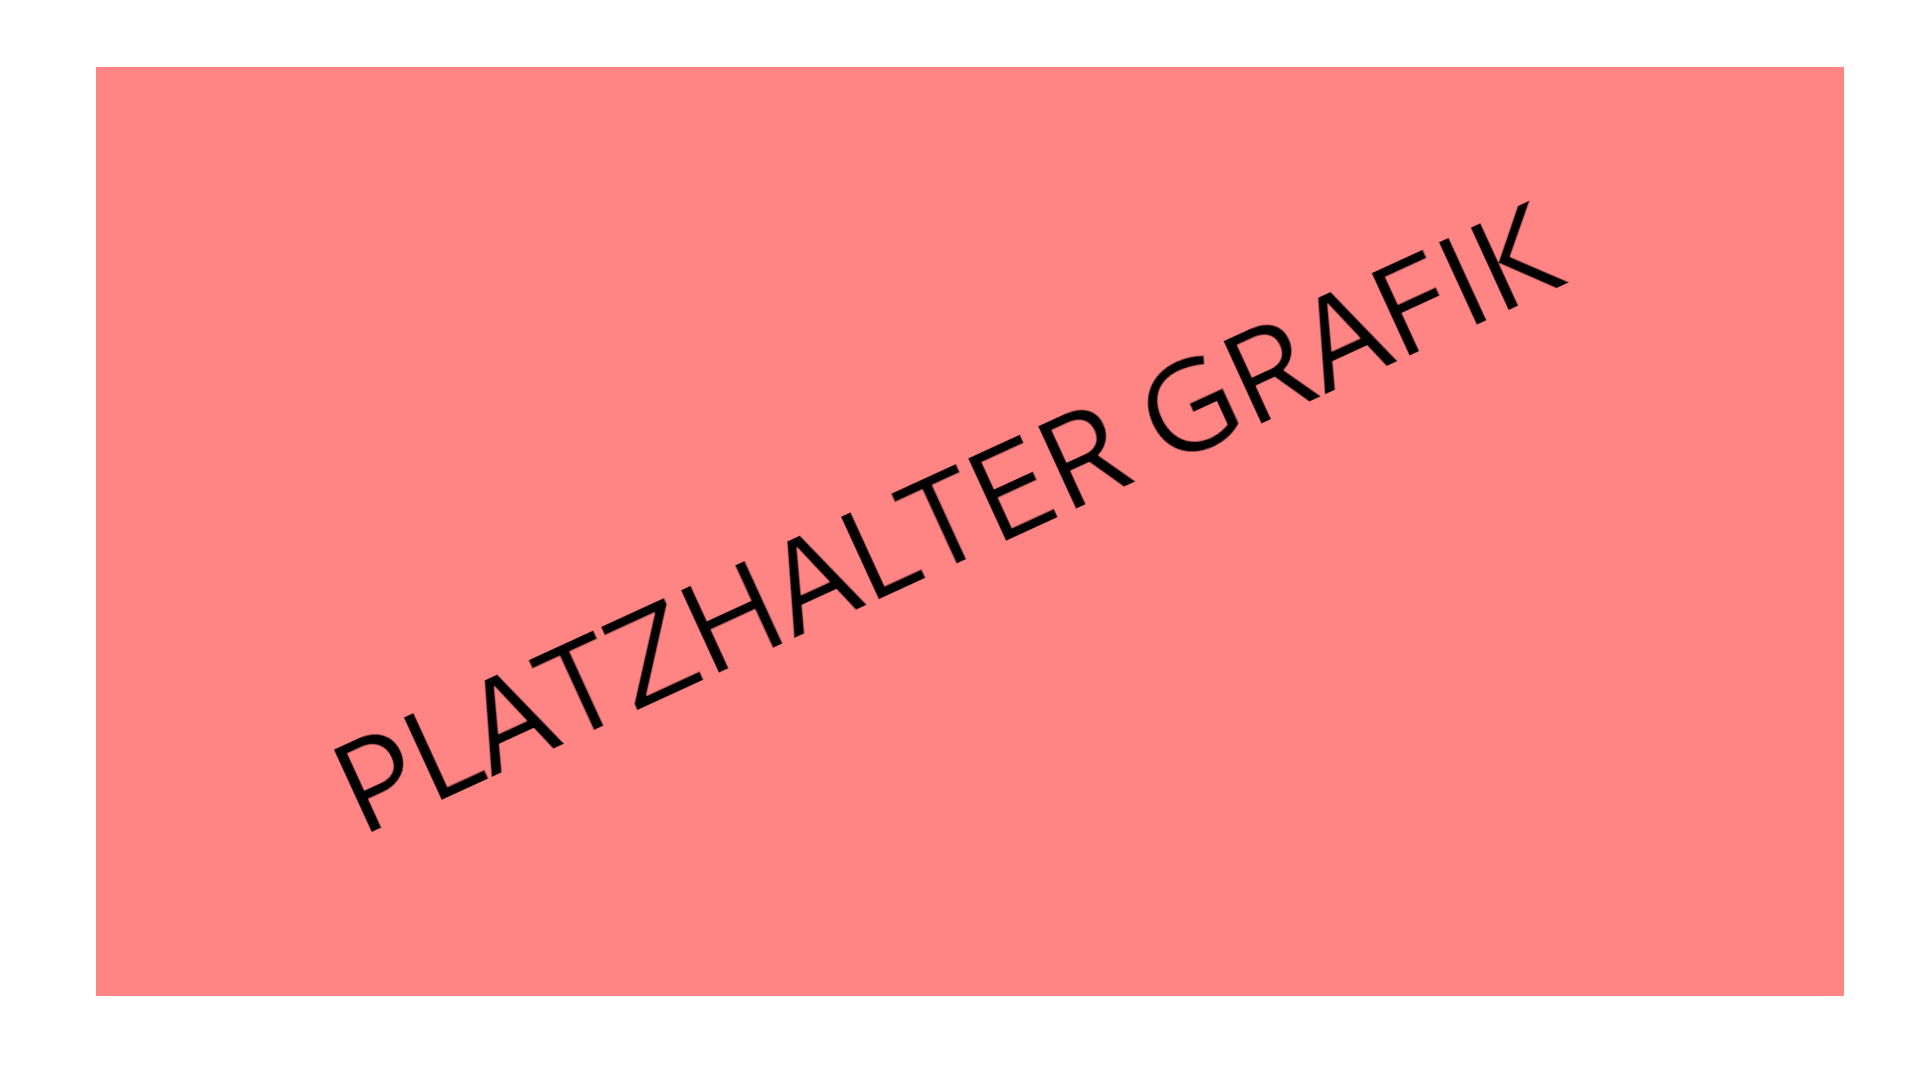
\includegraphics[height=6cm]{bilder/todo.png}
\captionof{figure}{Metamodell - Klassenname}
\end{center}

Eine Customer Supplier Beziehung ist eine Spezielle Beziehungen zwischen Kontexten aus welcher implizit festgelegt wird welcher Kontext sich welchem  Modell anzupassen hat.

\paragraph{Conformist}

%TODO Grafik machen
\begin{center}
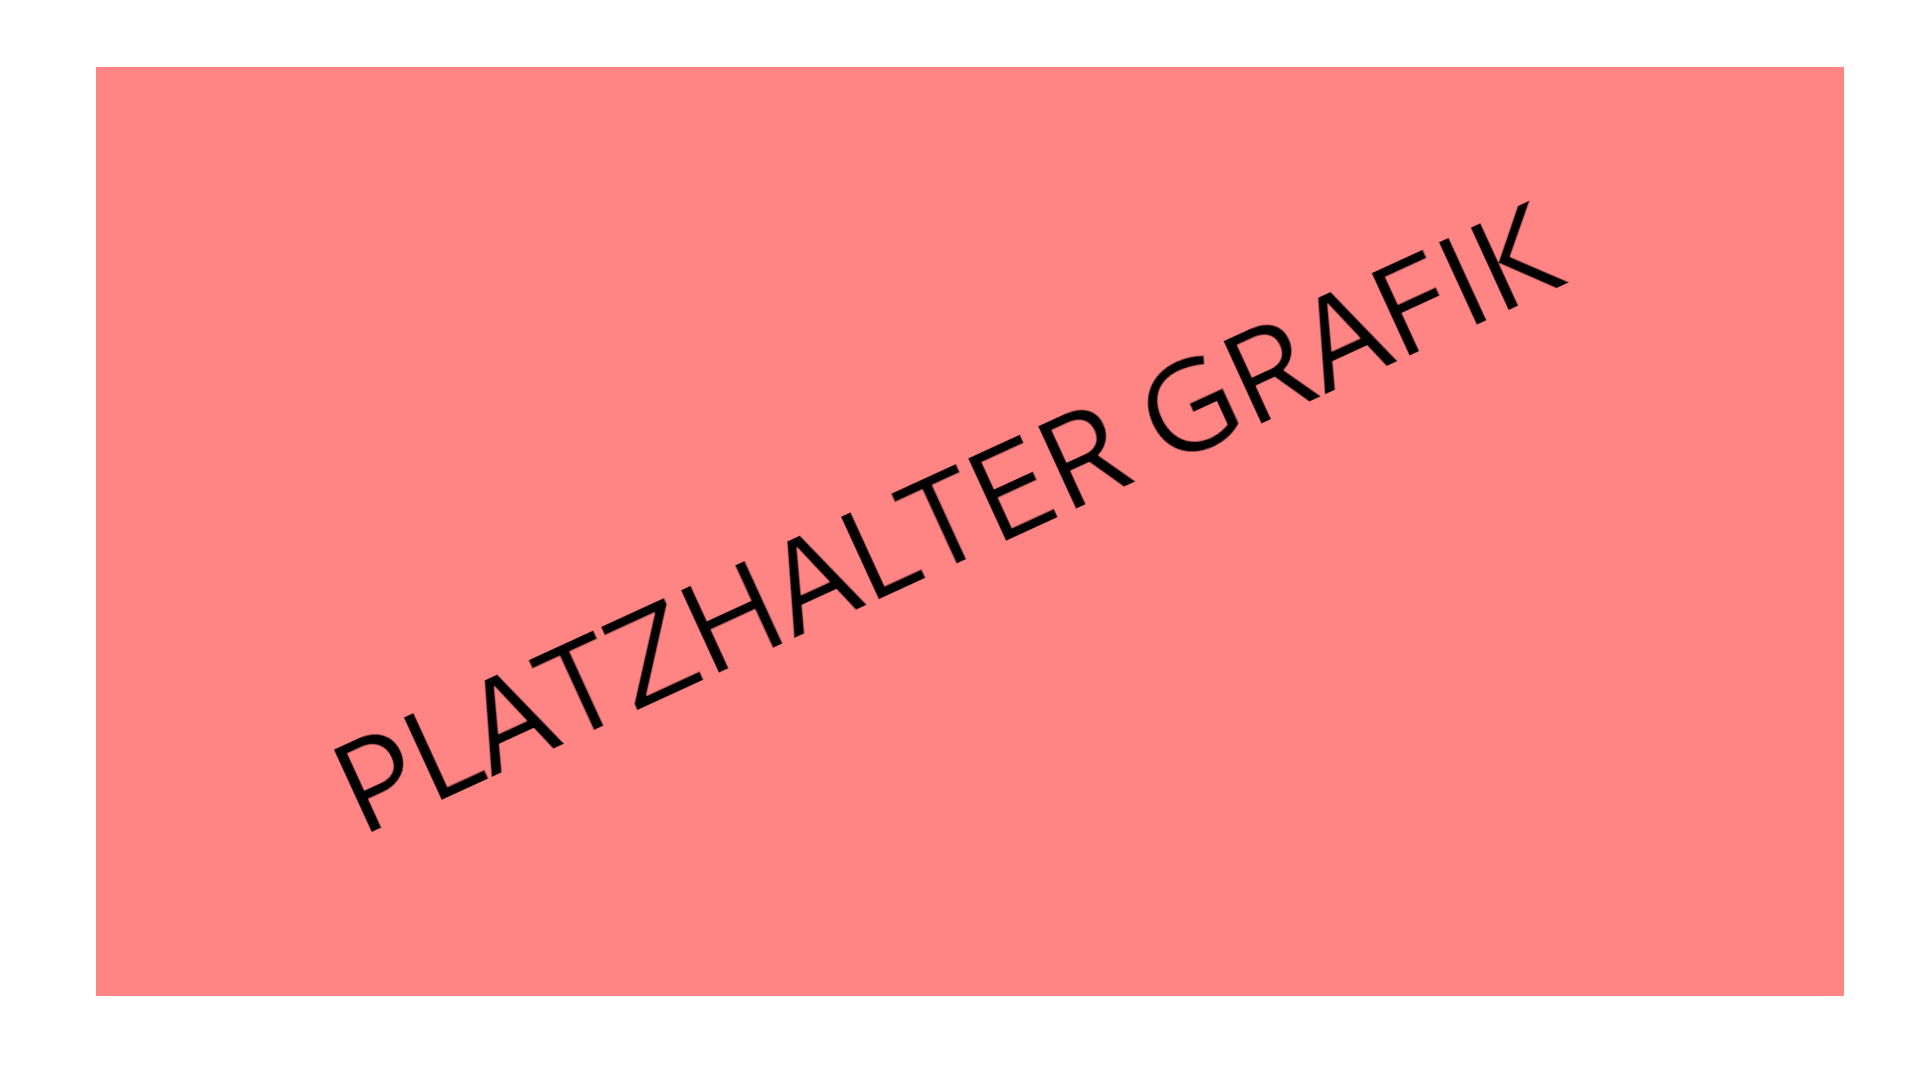
\includegraphics[height=6cm]{bilder/todo.png}
\captionof{figure}{Metamodell - Klassenname}
\end{center}

Eine Conformist Beziehung ist eine Spezielle Beziehungen zwischen Kontexten aus welcher implizit festgelegt wird welcher Kontext sich welchem  Modell anzupassen hat.

\newpage
\paragraph{Anticorruption Layer}

%TODO Grafik machen
\begin{center}
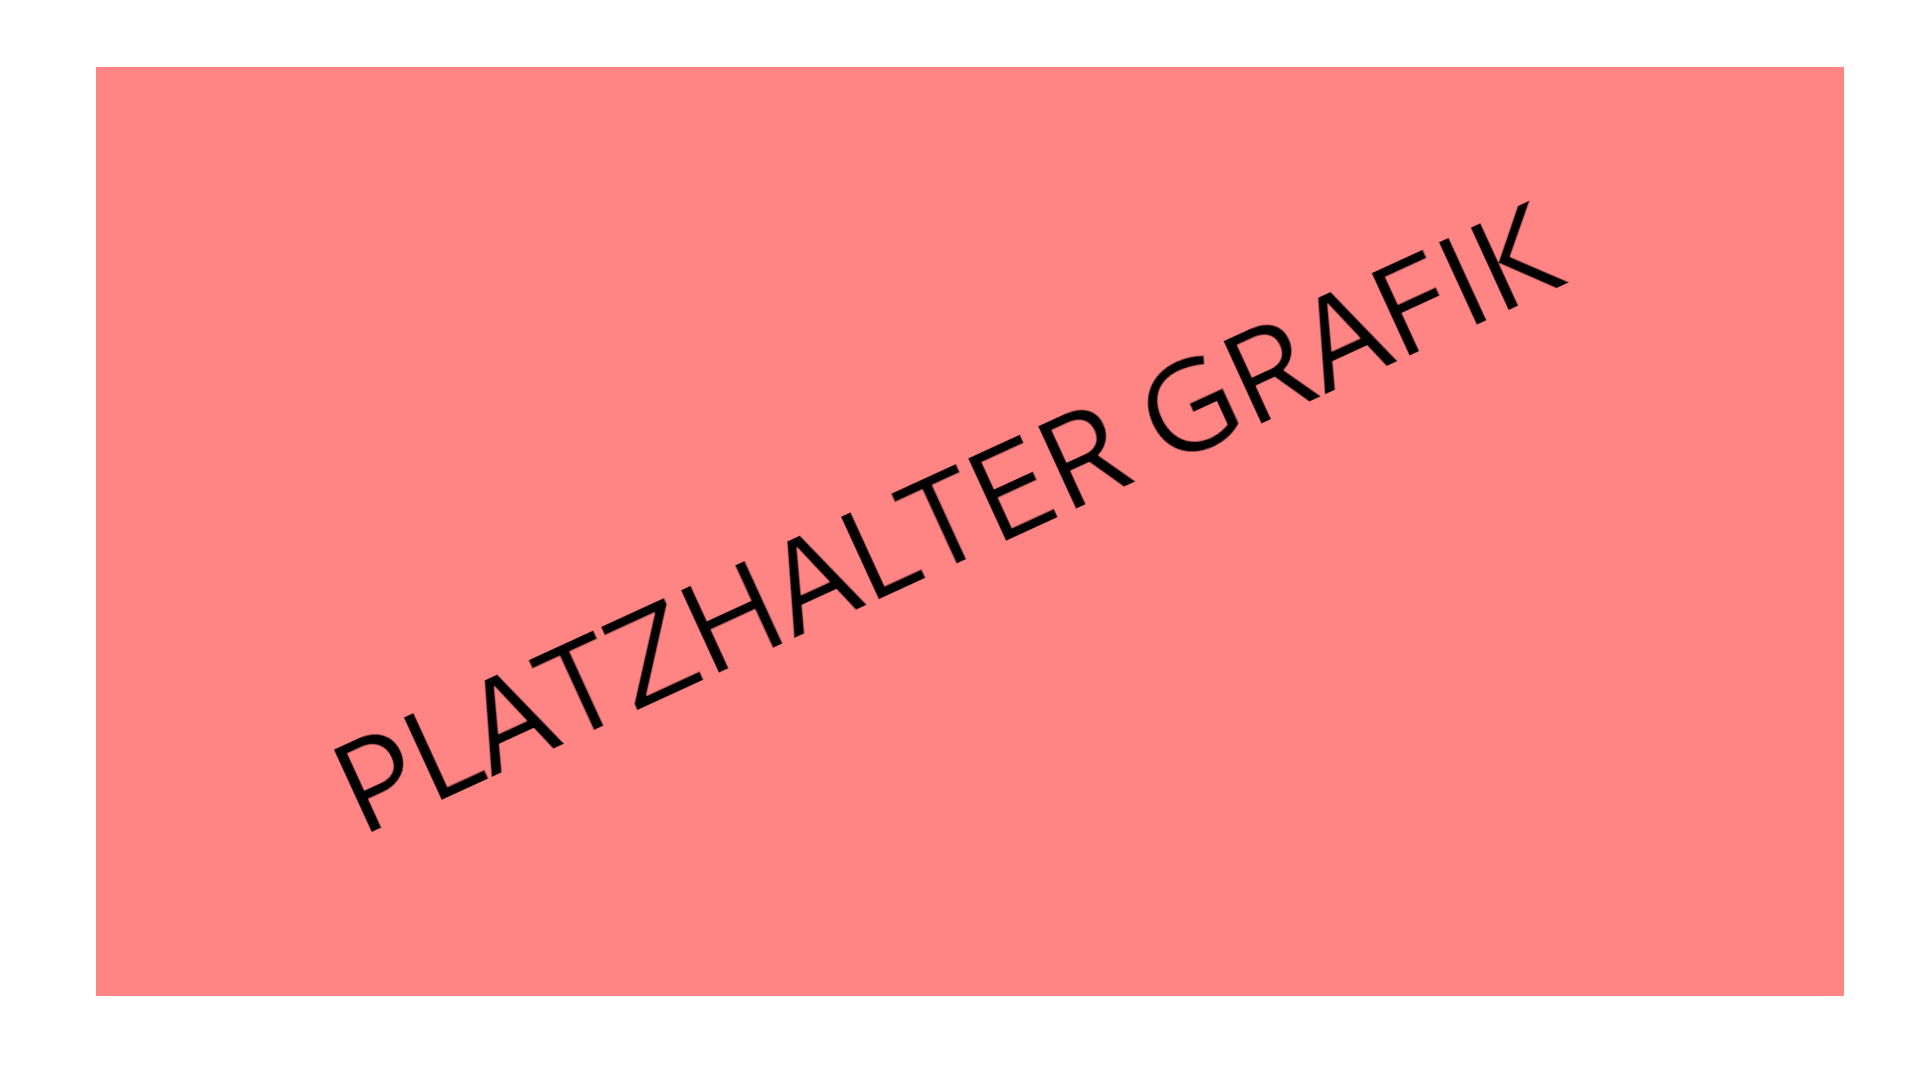
\includegraphics[height=6cm]{bilder/todo.png}
\captionof{figure}{Metamodell - Klassenname}
\end{center}

VGL Context Mapper

\paragraph{Open Host Service}

%TODO Grafik machen
\begin{center}
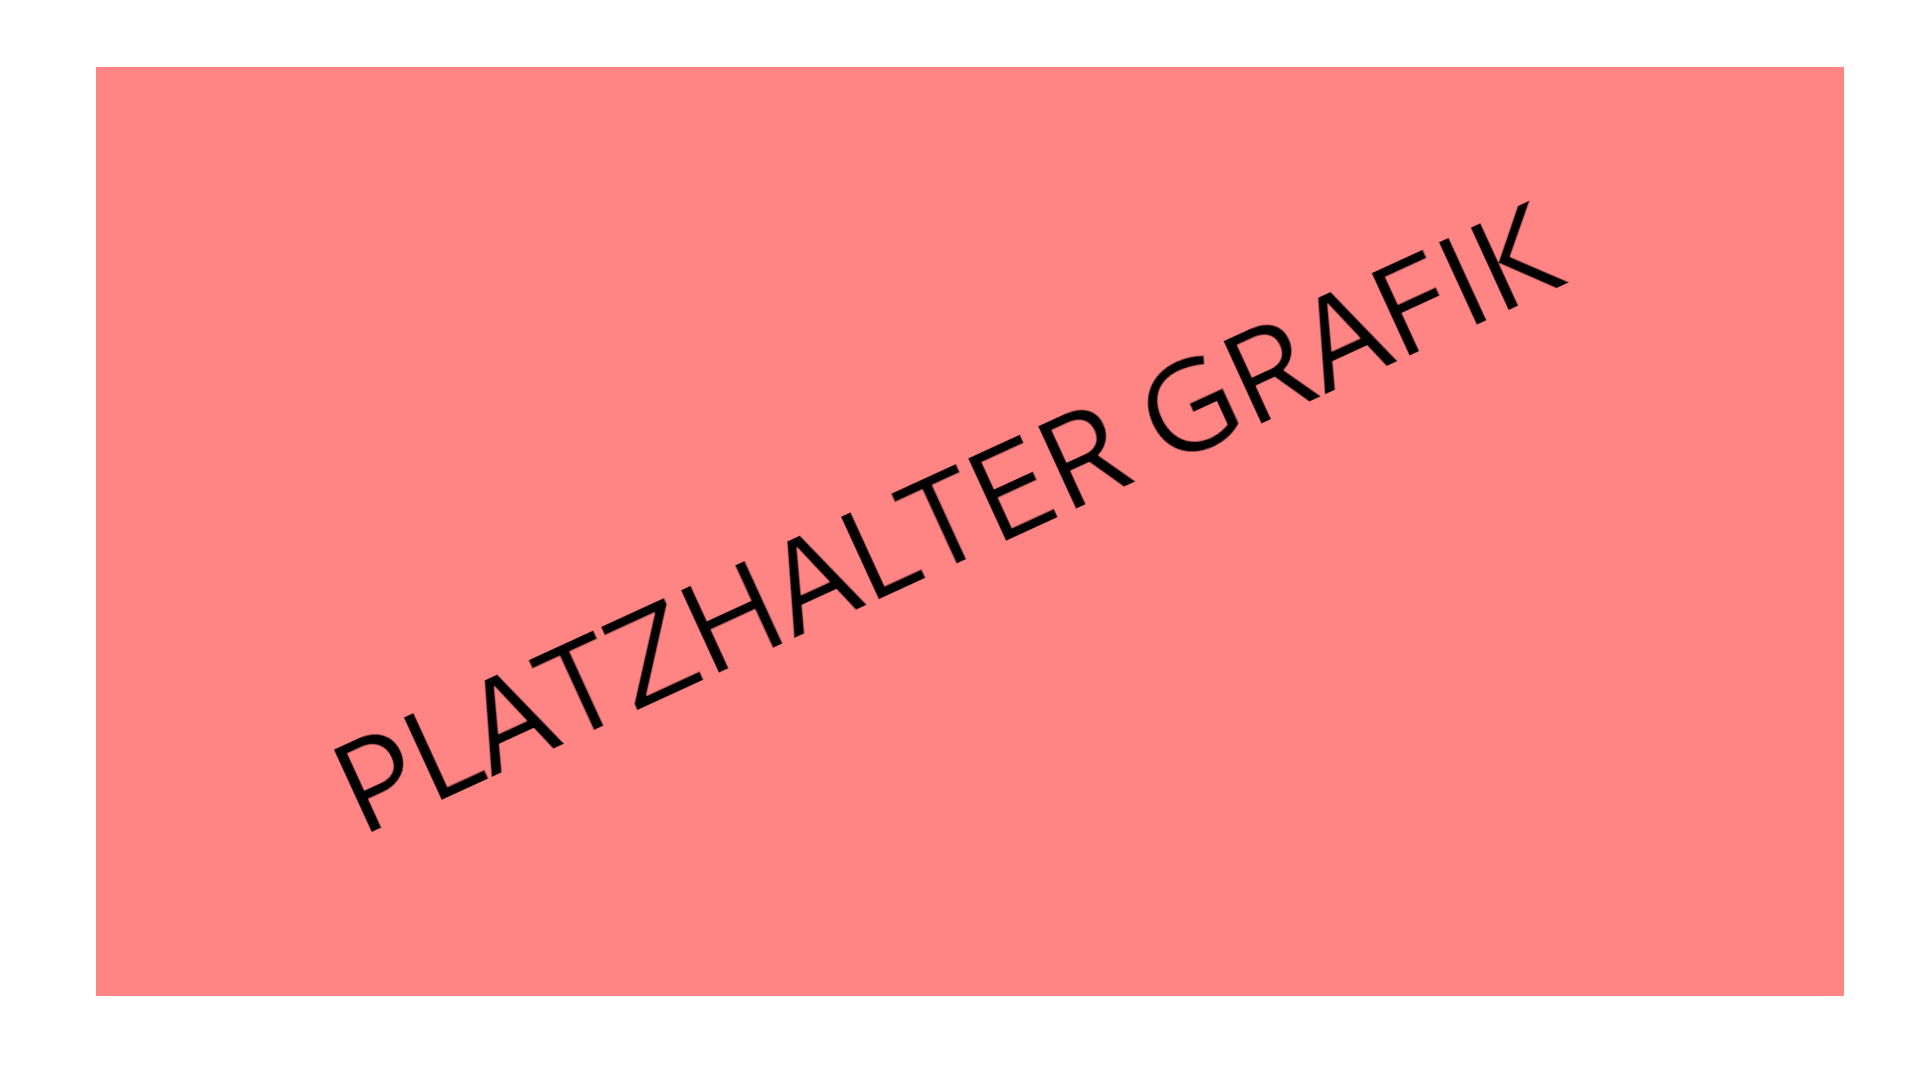
\includegraphics[height=6cm]{bilder/todo.png}
\captionof{figure}{Metamodell - Klassenname}
\end{center}

\newpage
VGL Context Mapper

\paragraph{Published Language}

%TODO Grafik machen
\begin{center}
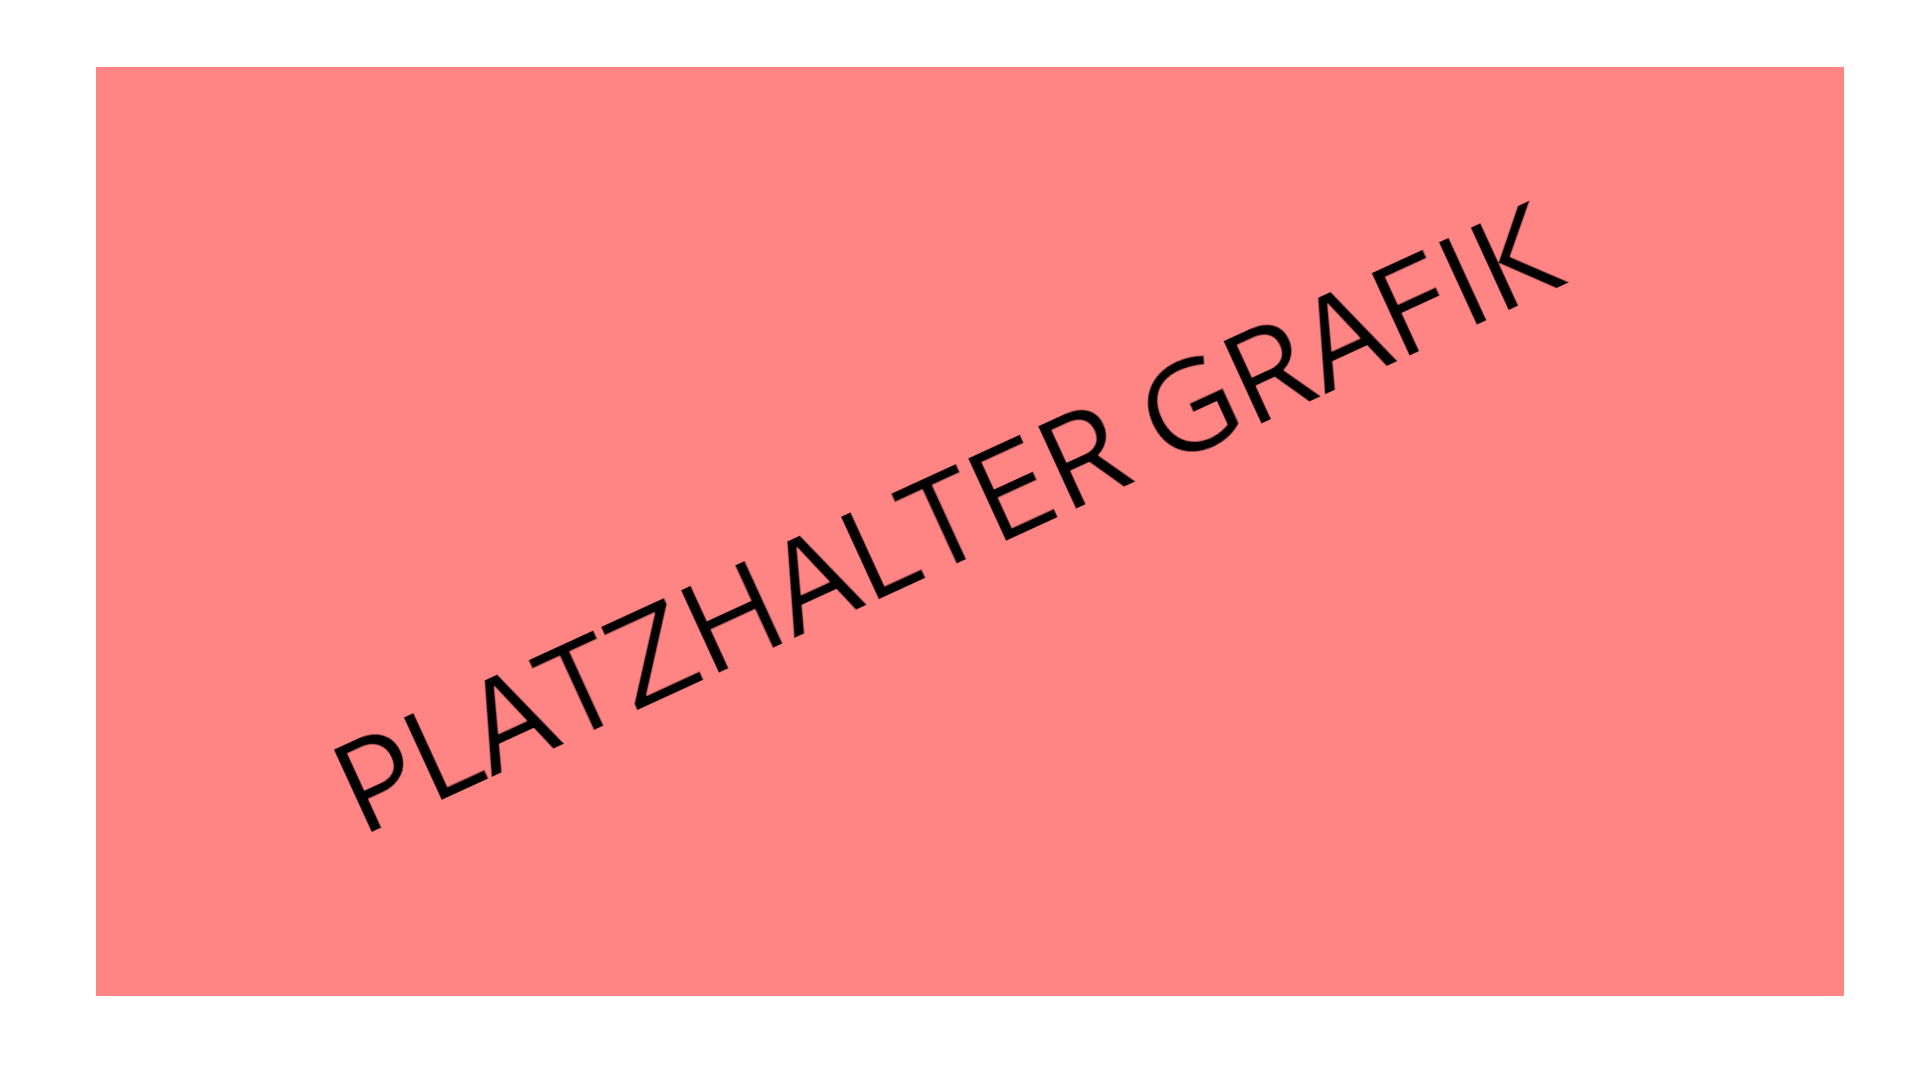
\includegraphics[height=6cm]{bilder/todo.png}
\captionof{figure}{Metamodell - Klassenname}
\end{center}

VGL Context Mapper

\paragraph{Seperate Ways}

Muss nicht modelliert werden

\newpage

\paragraph{Gesamtüberblick}

\begin{center}
\rotatebox{90}{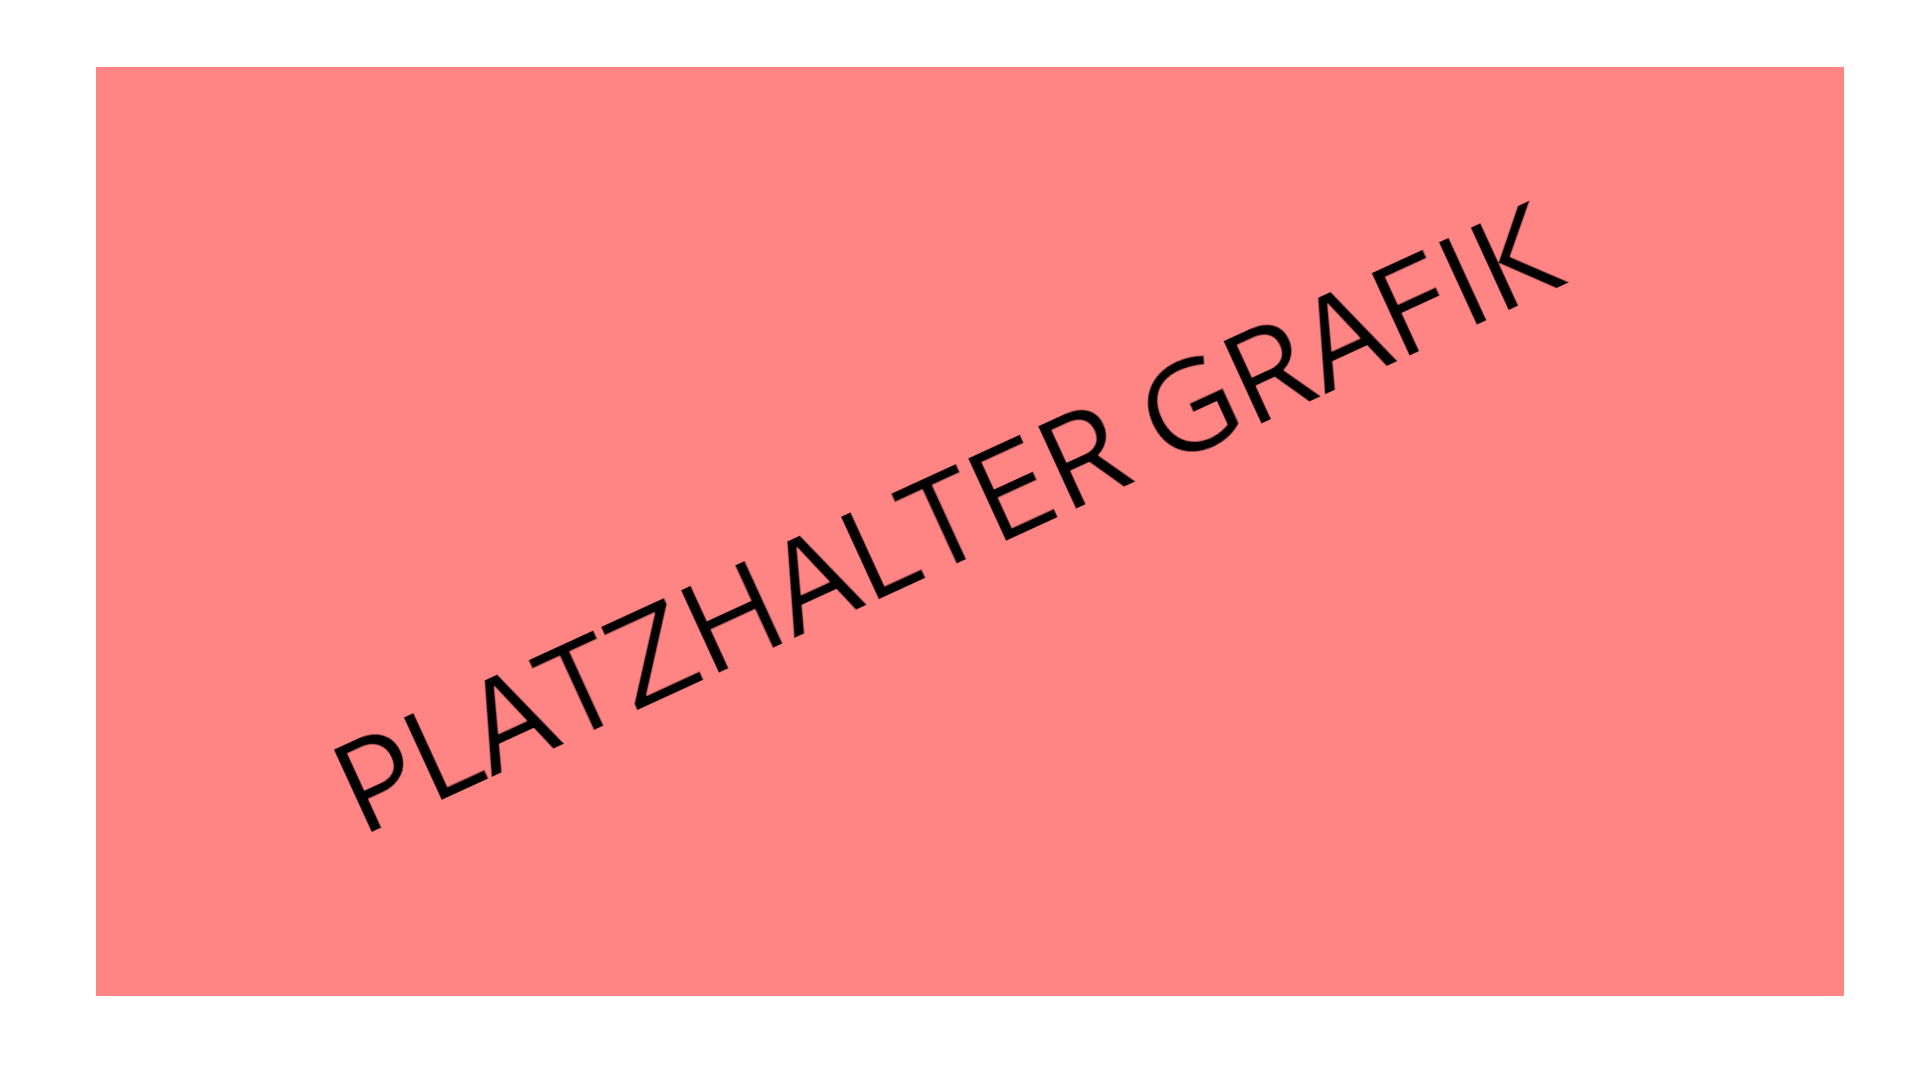
\includegraphics[height=10cm]{bilder/todo.png}}
\captionof{figure}{Metamodell - Klassenname}
\end{center}

%%%%%%%%%%%%%%%%%%%%%%%%%%%%%%%%%%%%%%%%%%%%%%%%%%%%%%%%%%%%%%%%%%%%%%%%%%%%%%%%%%%%%%%%%%%%%%%%%%%%%%%%%%%%%%%%%%%%
%			Techn
%%%%%%%%%%%%%%%%%%%%%%%%%%%%%%%%%%%%%%%%%%%%%%%%%%%%%%%%%%%%%%%%%%%%%%%%%%%%%%%%%%%%%%%%%%%%%%%%%%%%%%%%%%%%%%%%%%%%

\newpage
\subsection{Modellierung der technischen Umsetzung}

\subsubsection{Feinentwurf der technischen Schicht}

\paragraph{Microservice}

%TODO Grafik machen
\begin{center}
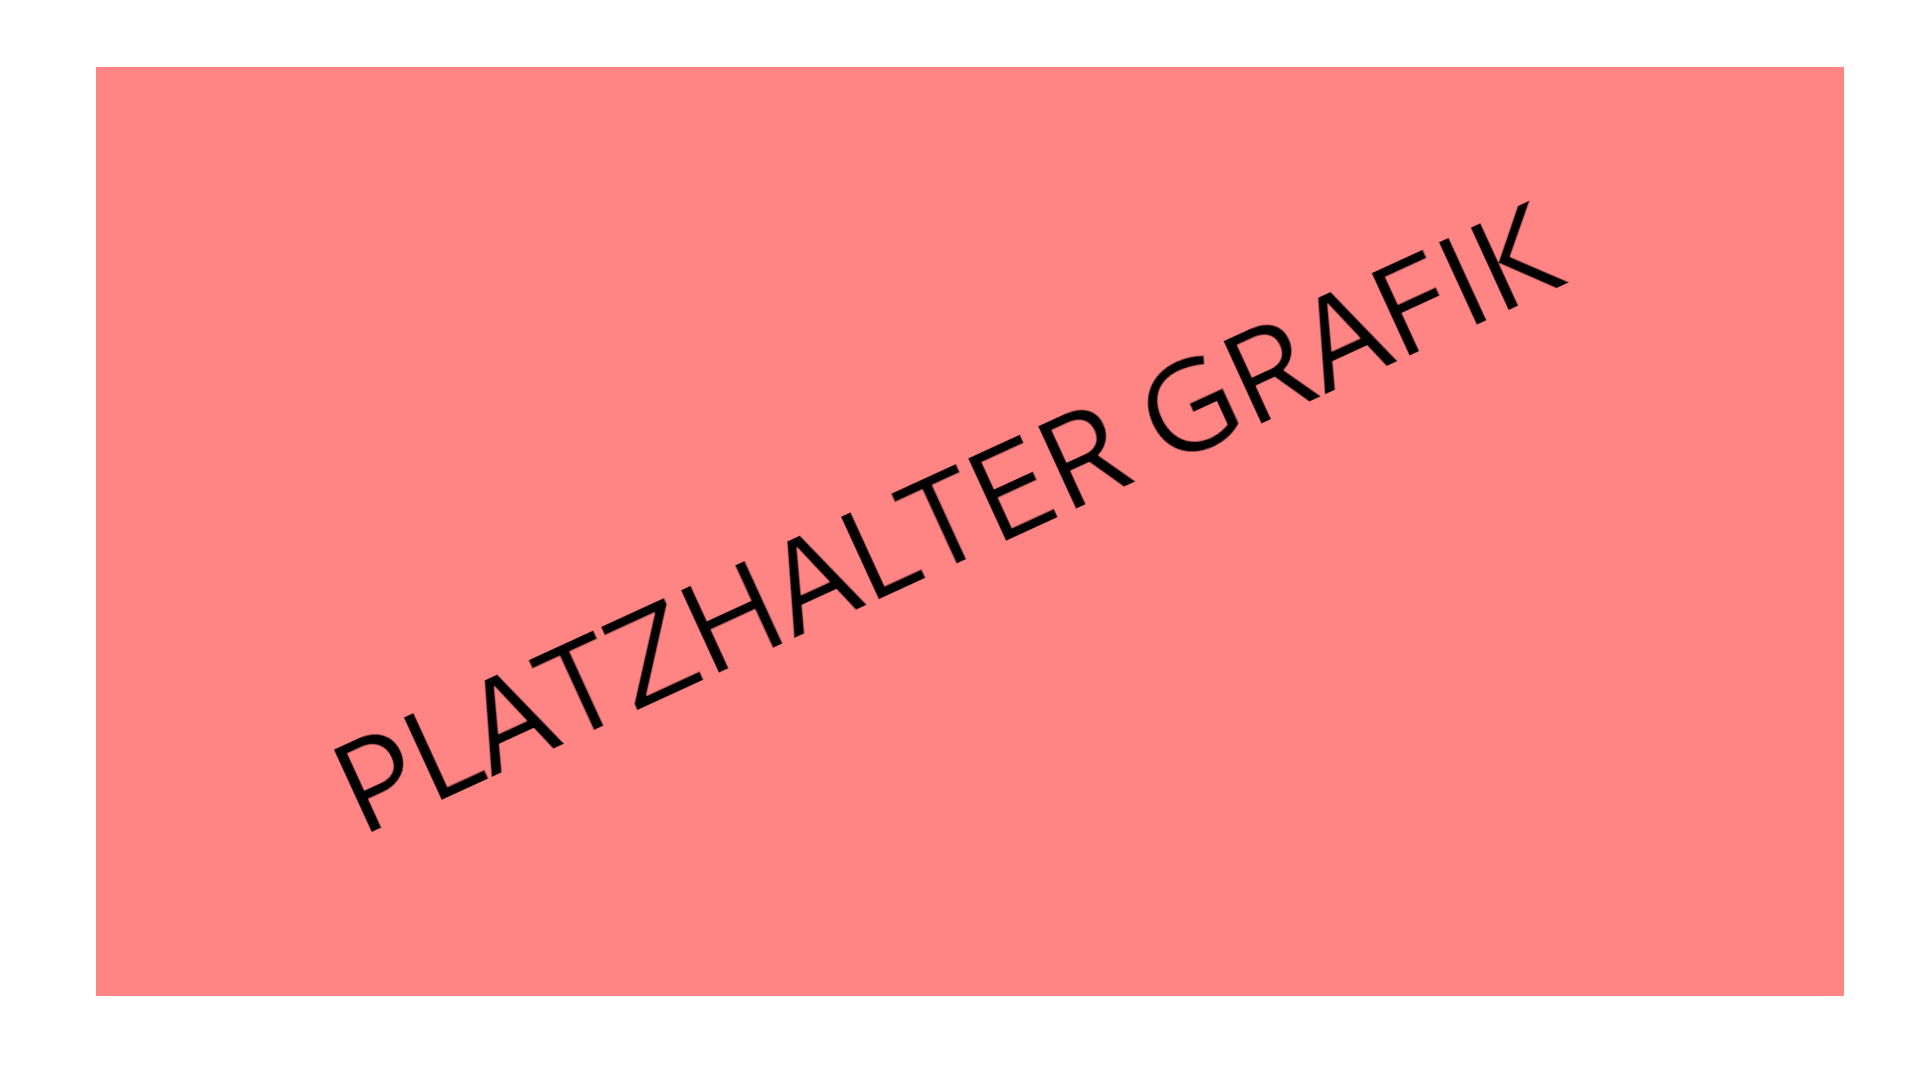
\includegraphics[height=6cm]{bilder/todo.png}
\captionof{figure}{Metamodell - Klassenname}
\end{center}

Lorem ipsum dolor sit amet, consetetur sadipscing elitr, sed diam nonumy eirmod tempor invidunt ut labore et dolore magna aliquyam erat, sed diam voluptua. At vero eos et accusam et justo duo dolores et ea rebum. Stet clita kasd gubergren, no sea takimata sanctus est Lorem ipsum dolor sit amet. Lorem ipsum dolor sit amet, consetetur sadipscing elitr, sed diam nonumy eirmod tempor invidunt ut labore et dolore magna aliquyam erat, sed diam voluptua. At vero eos et accusam et justo duo dolores et ea rebum. Stet clita kasd gubergren, no sea takimata sanctus est Lorem ipsum dolor sit amet. Lorem ipsum dolor sit amet, consetetur sadipscing elitr, sed diam nonumy eirmod tempor invidunt ut labore et dolore magna aliquyam erat, sed diam voluptua. At vero eos et accusam et justo duo dolores et ea rebum. Stet clita kasd gubergren, no sea takimata sanctus est Lorem ipsum dolor sit amet.   

Lorem ipsum dolor sit amet, consetetur sadipscing elitr, sed diam nonumy eirmod tempor invidunt ut labore et dolore magna aliquyam erat, sed diam voluptua. At vero eos et accusam et justo duo dolores et ea rebum. Stet clita kasd gubergren, no sea takimata sanctus est Lorem ipsum dolor sit amet. Lorem ipsum dolor sit amet, consetetur sadipscing elitr, sed diam nonumy eirmod tempor invidunt ut labore et dolore magna aliquyam erat, sed diam voluptua. At vero eos et accusam et justo duo dolores et ea rebum. Stet clita kasd gubergren, no sea takimata sanctus est Lorem ipsum dolor sit amet. Lorem ipsum dolor sit amet, consetetur sadipscing elitr, sed diam nonumy eirmod tempor invidunt ut labore et dolore magna aliquyam erat, sed diam voluptua. At vero eos et accusam et justo duo dolores et ea rebum. Stet clita kasd gubergren, no sea takimata sanctus est Lorem ipsum dolor sit amet.   

\newpage
\paragraph{Entity}

%TODO Grafik machen
\begin{center}
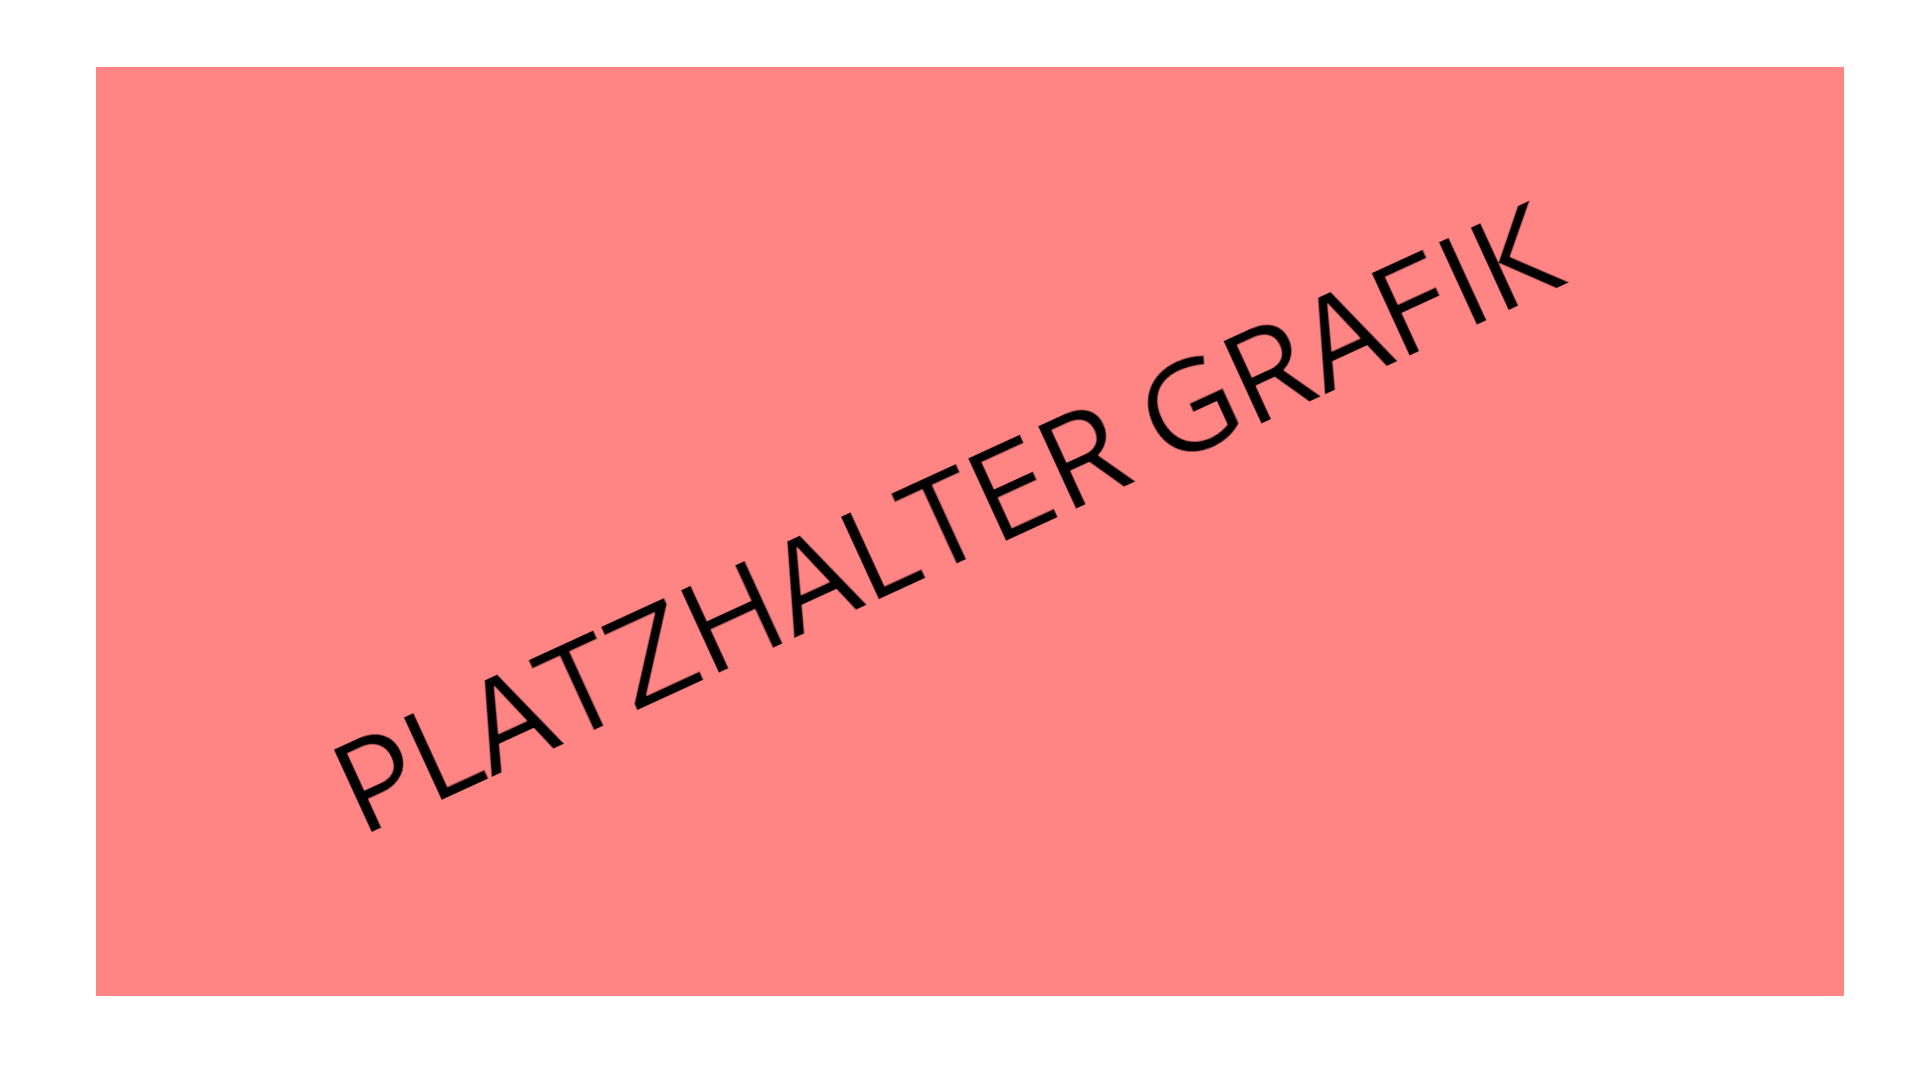
\includegraphics[height=6cm]{bilder/todo.png}
\captionof{figure}{Metamodell - Klassenname}
\end{center}

Lorem ipsum dolor sit amet, consetetur sadipscing elitr, sed diam nonumy eirmod tempor invidunt ut labore et dolore magna aliquyam erat, sed diam voluptua. At vero eos et accusam et justo duo dolores et ea rebum. Stet clita kasd gubergren, no sea takimata sanctus est Lorem ipsum dolor sit amet. Lorem ipsum dolor sit amet, consetetur sadipscing elitr, sed diam nonumy eirmod tempor invidunt ut labore et dolore magna aliquyam erat, sed diam voluptua.

\paragraph{Service Klasse}

%TODO Grafik machen
\begin{center}
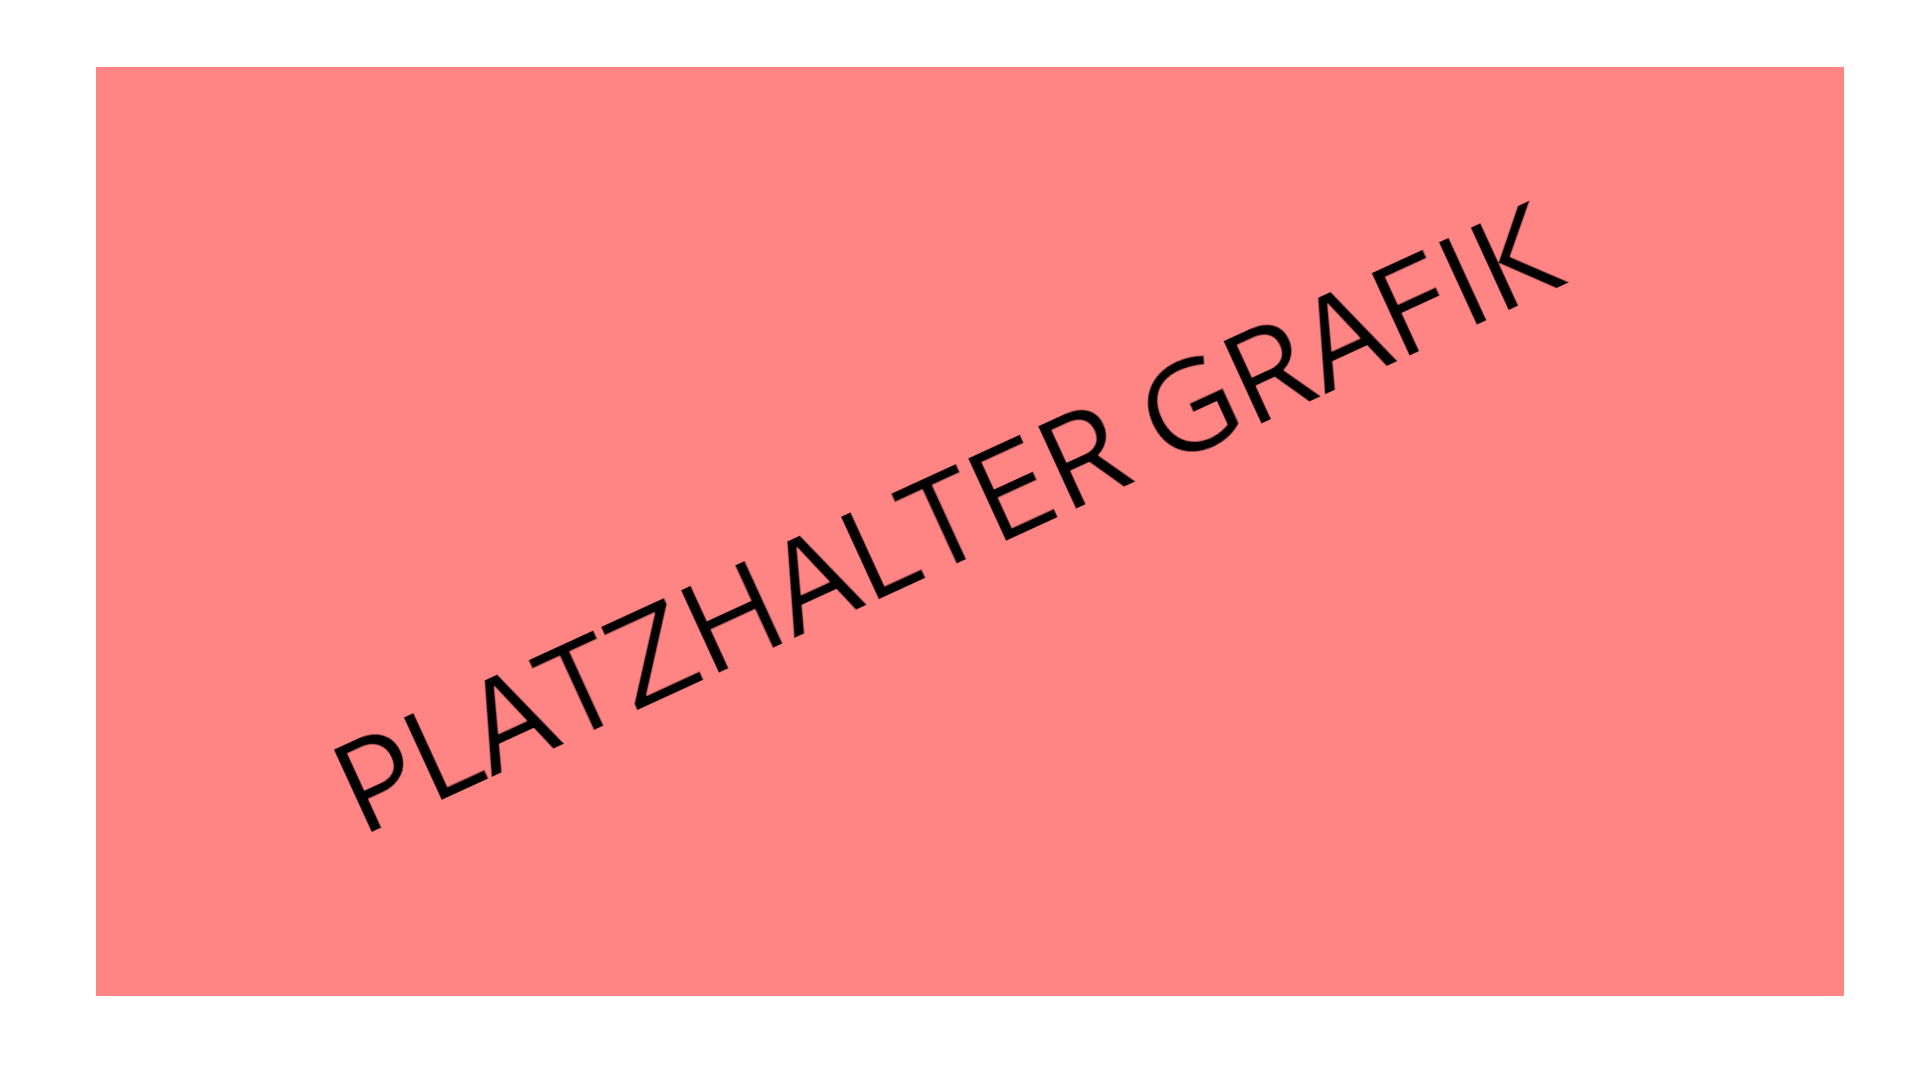
\includegraphics[height=6cm]{bilder/todo.png}
\captionof{figure}{Metamodell - Klassenname}
\end{center}

Lorem ipsum dolor sit amet, consetetur sadipscing elitr, sed diam nonumy eirmod tempor invidunt ut labore et dolore magna aliquyam erat, sed diam voluptua. At vero eos et accusam et justo duo dolores et ea rebum. Stet clita kasd gubergren, no sea takimata sanctus est Lorem ipsum dolor sit amet. Lorem ipsum dolor sit amet, consetetur sadipscing elitr, sed diam nonumy eirmod tempor invidunt ut labore et dolore magna aliquyam erat, sed diam voluptua.  

\newpage
\paragraph{Repository}

%TODO Grafik machen
\begin{center}
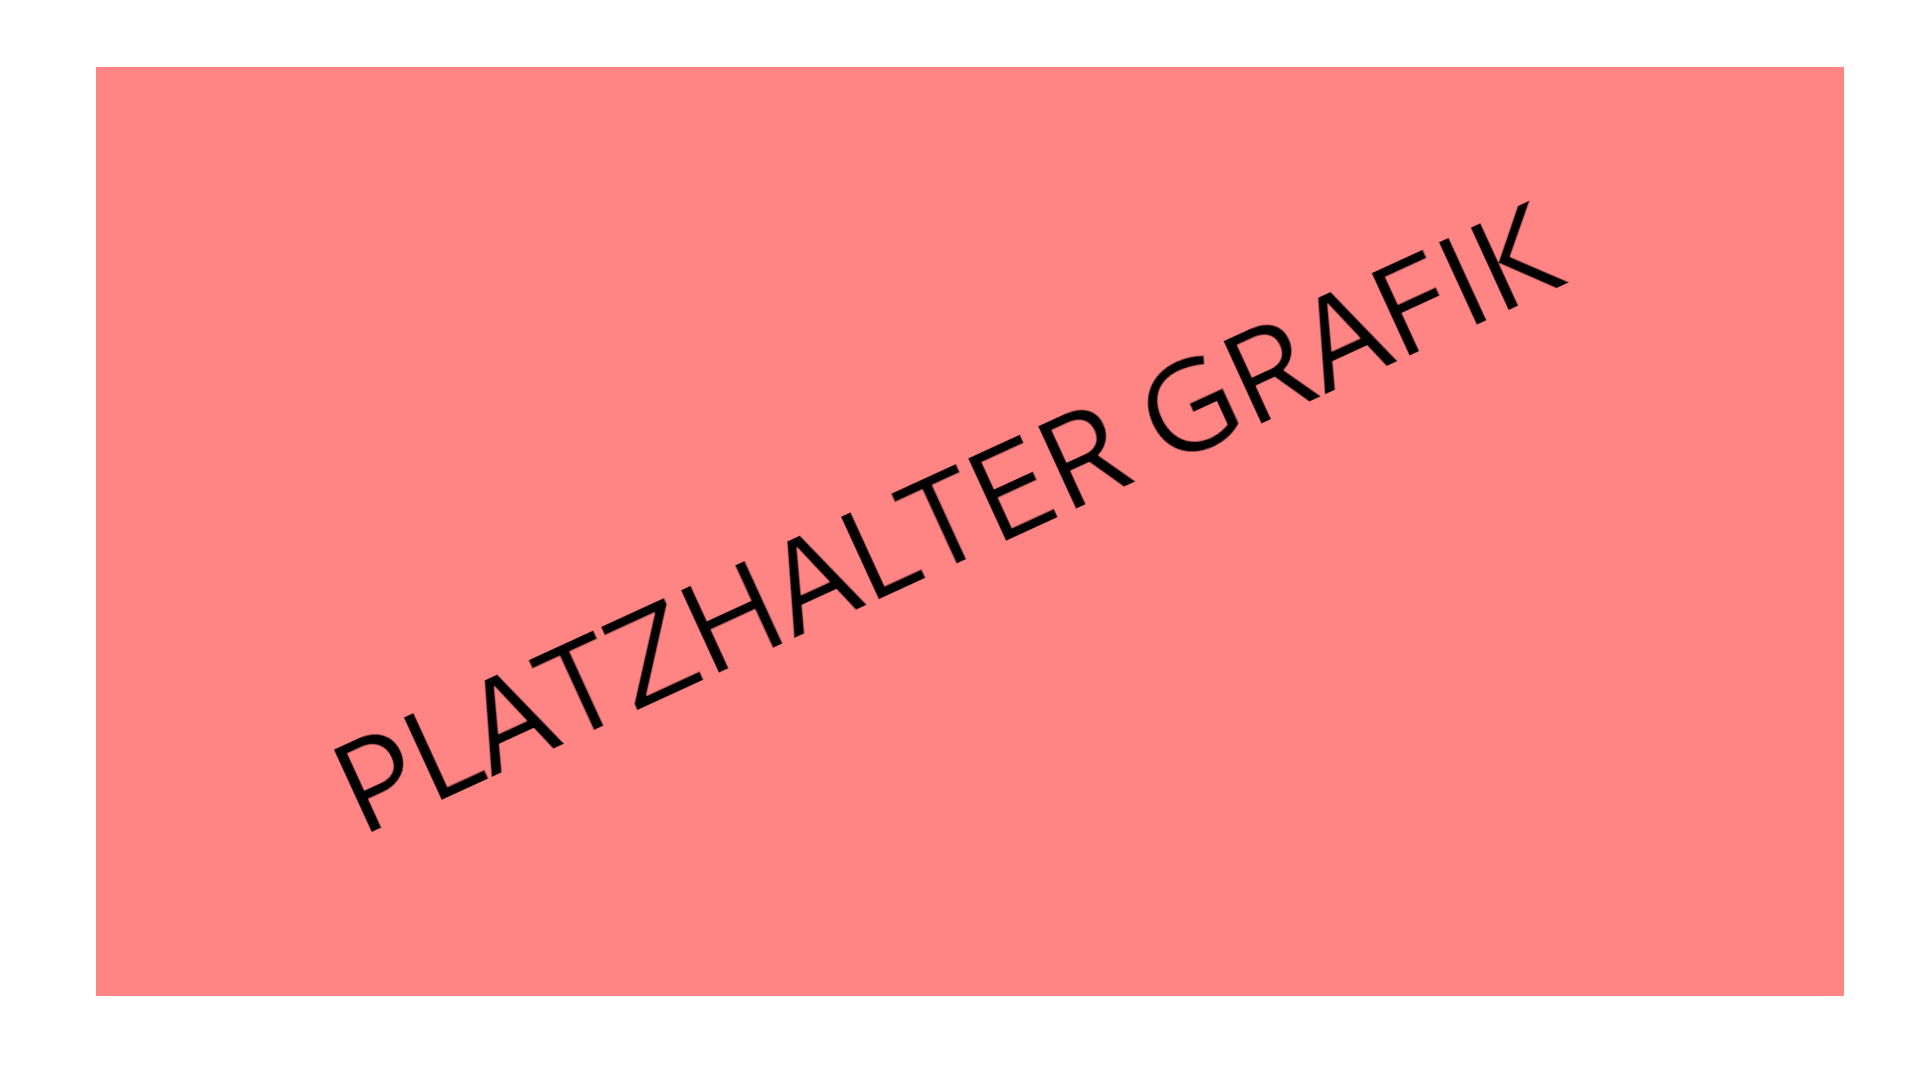
\includegraphics[height=6cm]{bilder/todo.png}
\captionof{figure}{Metamodell - Klassenname}
\end{center}

Lorem ipsum dolor sit amet, consetetur sadipscing elitr, sed diam nonumy eirmod tempor invidunt ut labore et dolore magna aliquyam erat, sed diam voluptua. At vero eos et accusam et justo duo dolores et ea rebum. Stet clita kasd gubergren, no sea takimata sanctus est Lorem ipsum dolor sit amet. Lorem ipsum dolor sit amet, consetetur sadipscing elitr, sed diam nonumy eirmod tempor invidunt ut labore et dolore magna aliquyam erat, sed diam voluptua. 

\paragraph{Schnittstelle}

%TODO Grafik machen
\begin{center}
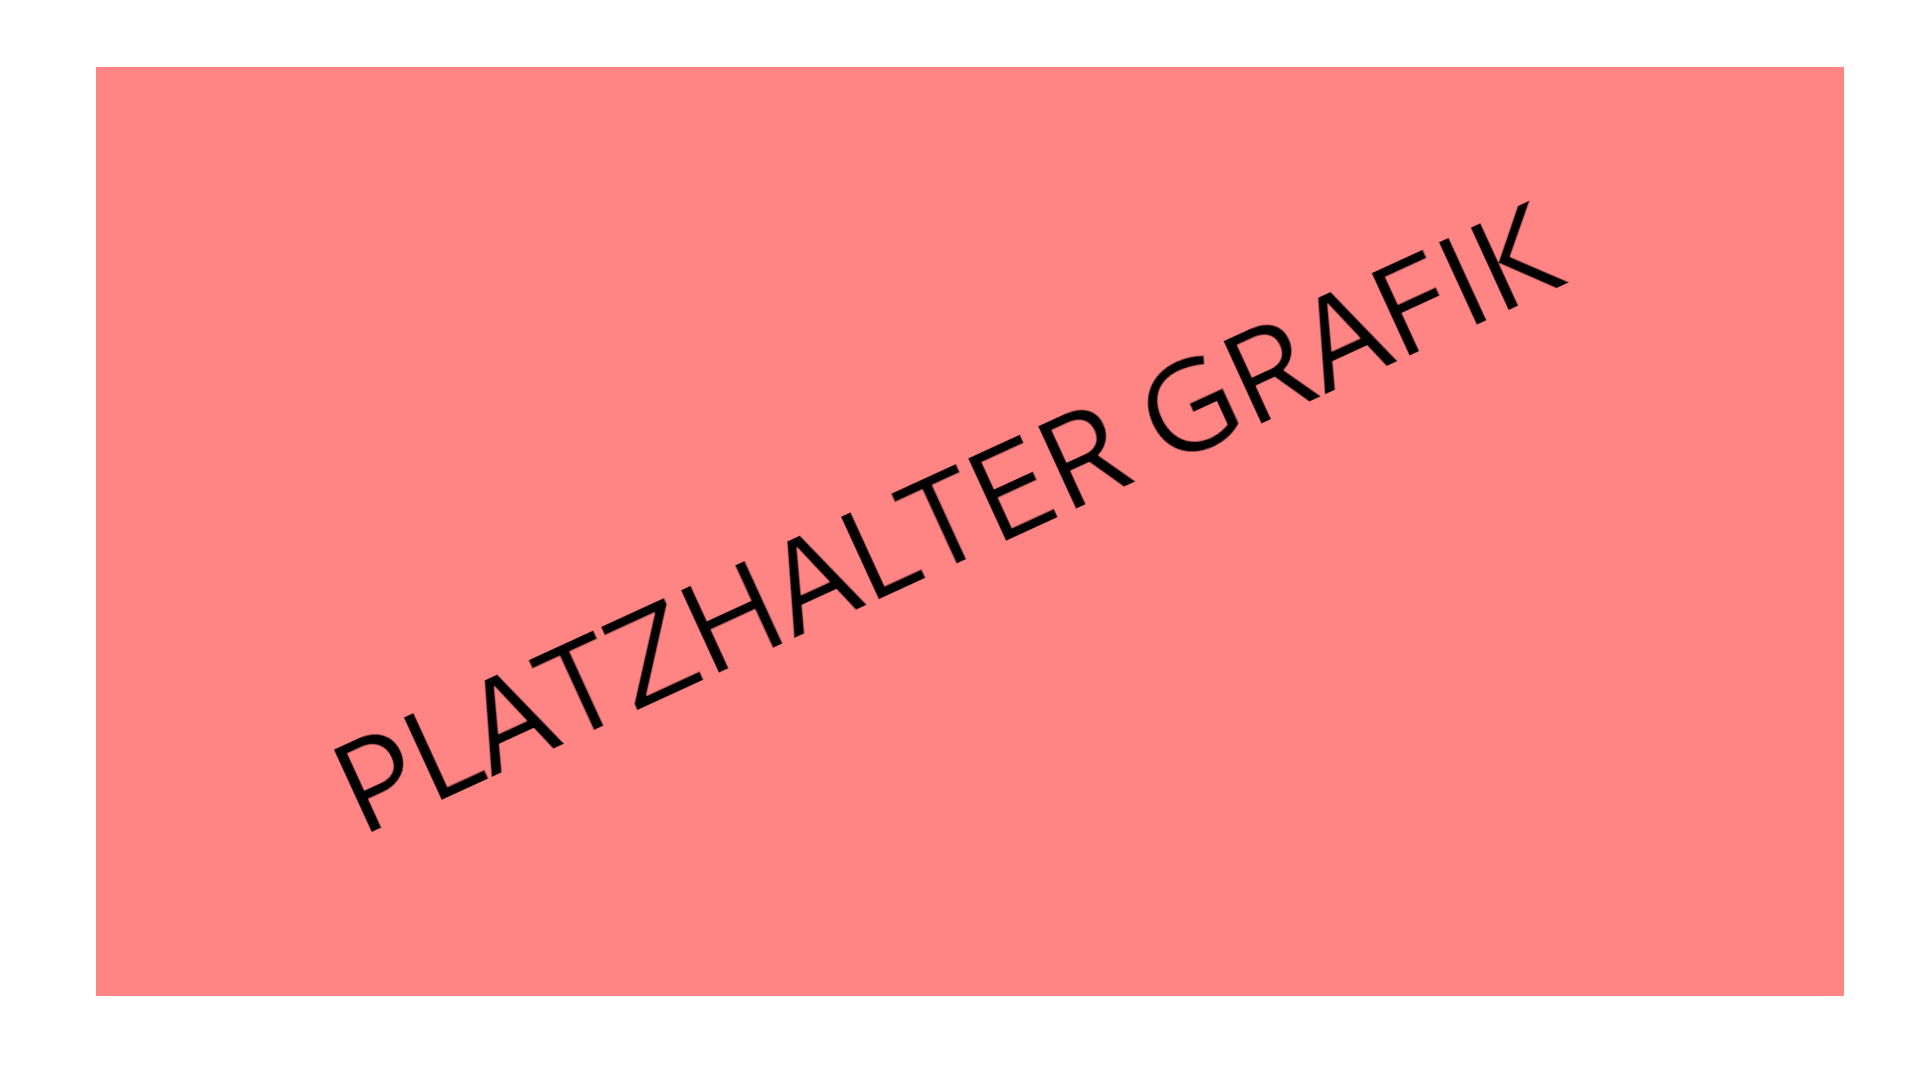
\includegraphics[height=6cm]{bilder/todo.png}
\captionof{figure}{Metamodell - Klassenname}
\end{center}

Lorem ipsum dolor sit amet, consetetur sadipscing elitr, sed diam nonumy eirmod tempor invidunt ut labore et dolore magna aliquyam erat, sed diam voluptua. At vero eos et accusam et justo duo dolores et ea rebum. Stet clita kasd gubergren, no sea takimata sanctus est Lorem ipsum dolor sit amet. Lorem ipsum dolor sit amet, consetetur sadipscing elitr, sed diam nonumy eirmod tempor invidunt ut labore et dolore magna aliquyam erat, sed diam voluptua.

\newpage
\paragraph{Synchrone Schnittstelle}

%TODO Grafik machen
\begin{center}
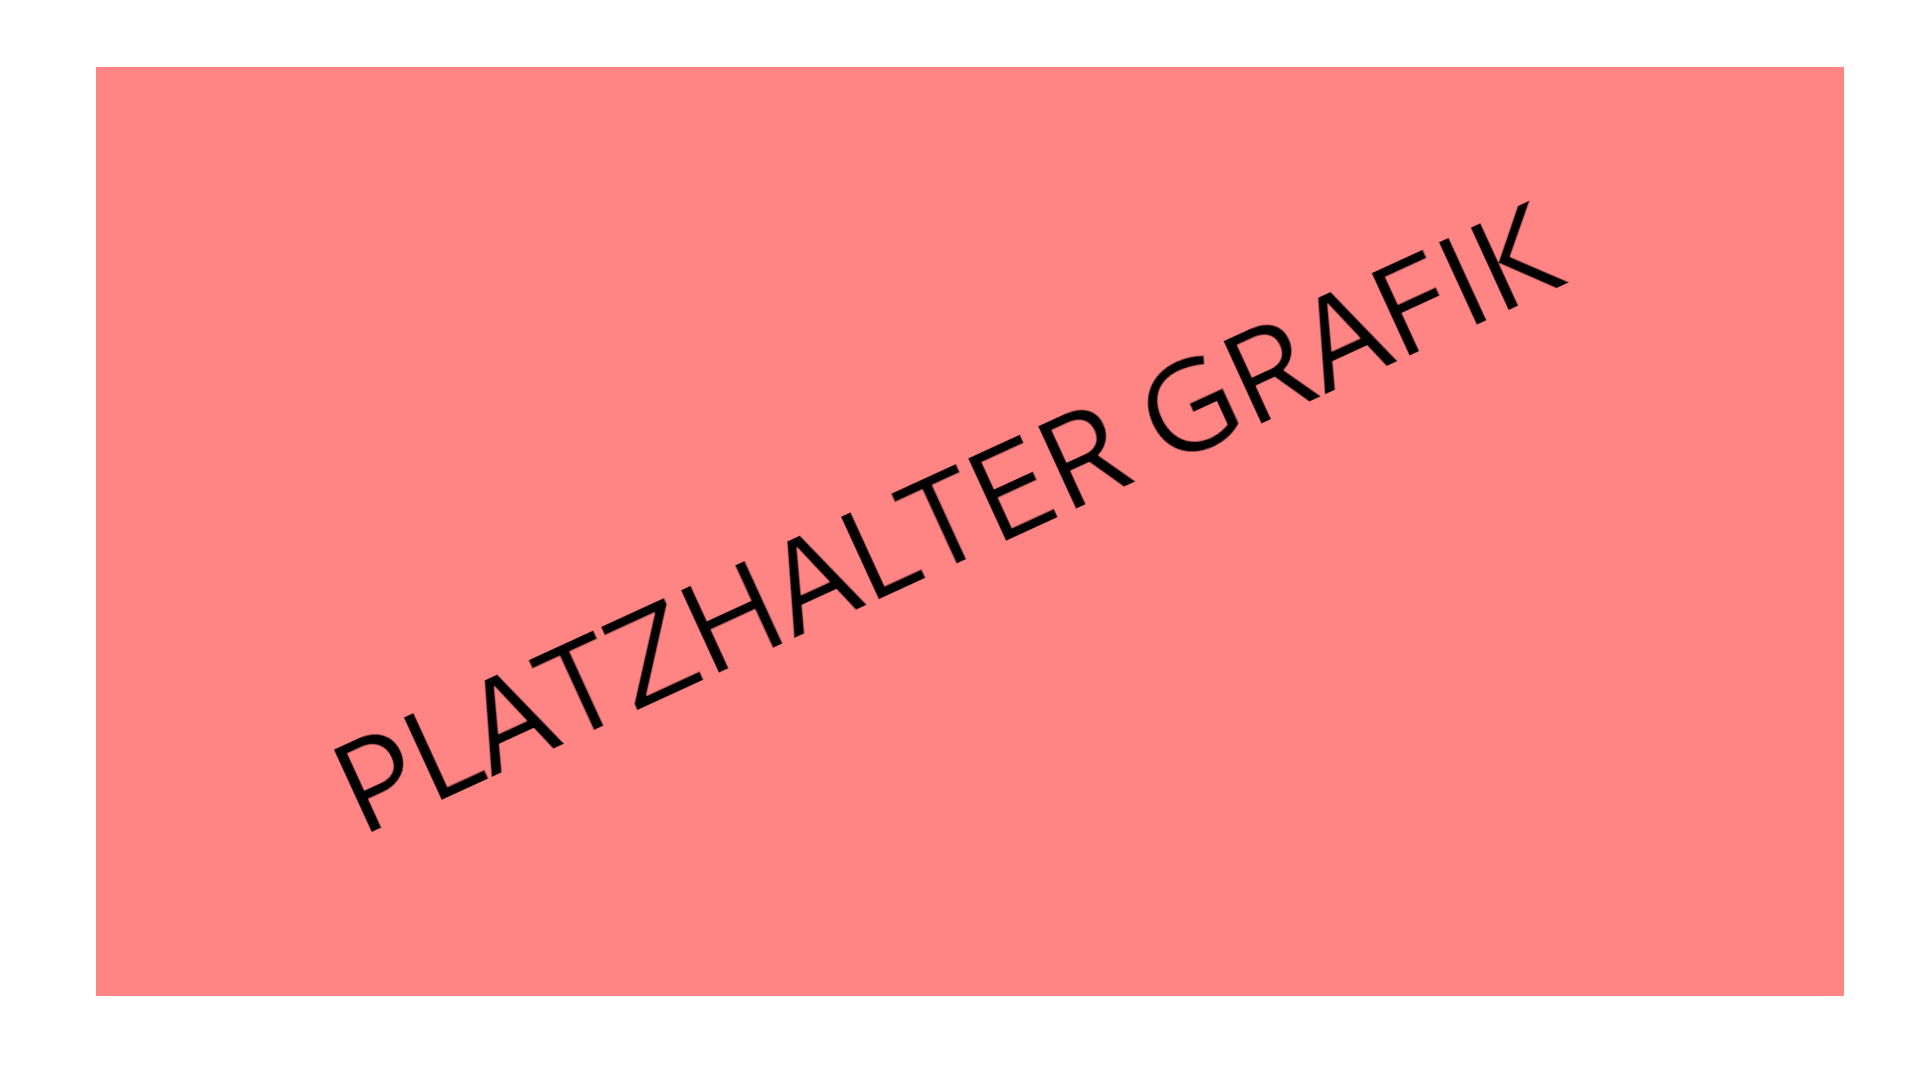
\includegraphics[height=6cm]{bilder/todo.png}
\captionof{figure}{Metamodell - Klassenname}
\end{center}

Lorem ipsum dolor sit amet, consetetur sadipscing elitr, sed diam nonumy eirmod tempor invidunt ut labore et dolore magna aliquyam erat, sed diam voluptua. At vero eos et accusam et justo duo dolores et ea rebum. Stet clita kasd gubergren, no sea takimata sanctus est Lorem ipsum dolor sit amet. Lorem ipsum dolor sit amet, consetetur sadipscing elitr, sed diam nonumy eirmod tempor invidunt ut labore et dolore magna aliquyam erat, sed diam voluptua. At vero eos et accusam et justo duo dolores et ea rebum. Stet clita kasd gubergren, no sea takimata sanctus est Lorem ipsum dolor sit amet. Lorem ipsum dolor sit amet, consetetur sadipscing elitr, sed diam nonumy eirmod tempor invidunt ut labore et dolore magna aliquyam erat, sed diam voluptua. At vero eos et accusam et justo duo dolores et ea rebum. Stet clita kasd gubergren, no sea takimata sanctus est Lorem ipsum dolor sit amet.   

Lorem ipsum dolor sit amet, consetetur sadipscing elitr, sed diam nonumy eirmod tempor invidunt ut labore et dolore magna aliquyam erat, sed diam voluptua. At vero eos et accusam et justo duo dolores et ea rebum. Stet clita kasd gubergren, no sea takimata sanctus est Lorem ipsum dolor sit amet. Lorem ipsum dolor sit amet, consetetur sadipscing elitr, sed diam nonumy eirmod tempor invidunt ut labore et dolore magna aliquyam erat, sed diam voluptua. At vero eos et accusam et justo duo dolores et ea rebum. Stet clita kasd gubergren, no sea takimata sanctus est Lorem ipsum dolor sit amet. Lorem ipsum dolor sit amet, consetetur sadipscing elitr, sed diam nonumy eirmod tempor invidunt ut labore et dolore magna aliquyam erat, sed diam voluptua. At vero eos et accusam et justo duo dolores et ea rebum. Stet clita kasd gubergren, no sea takimata sanctus est Lorem ipsum dolor sit amet.   
 

\newpage
\paragraph{Asynchrone Schnittstelle}

%TODO Grafik machen
\begin{center}
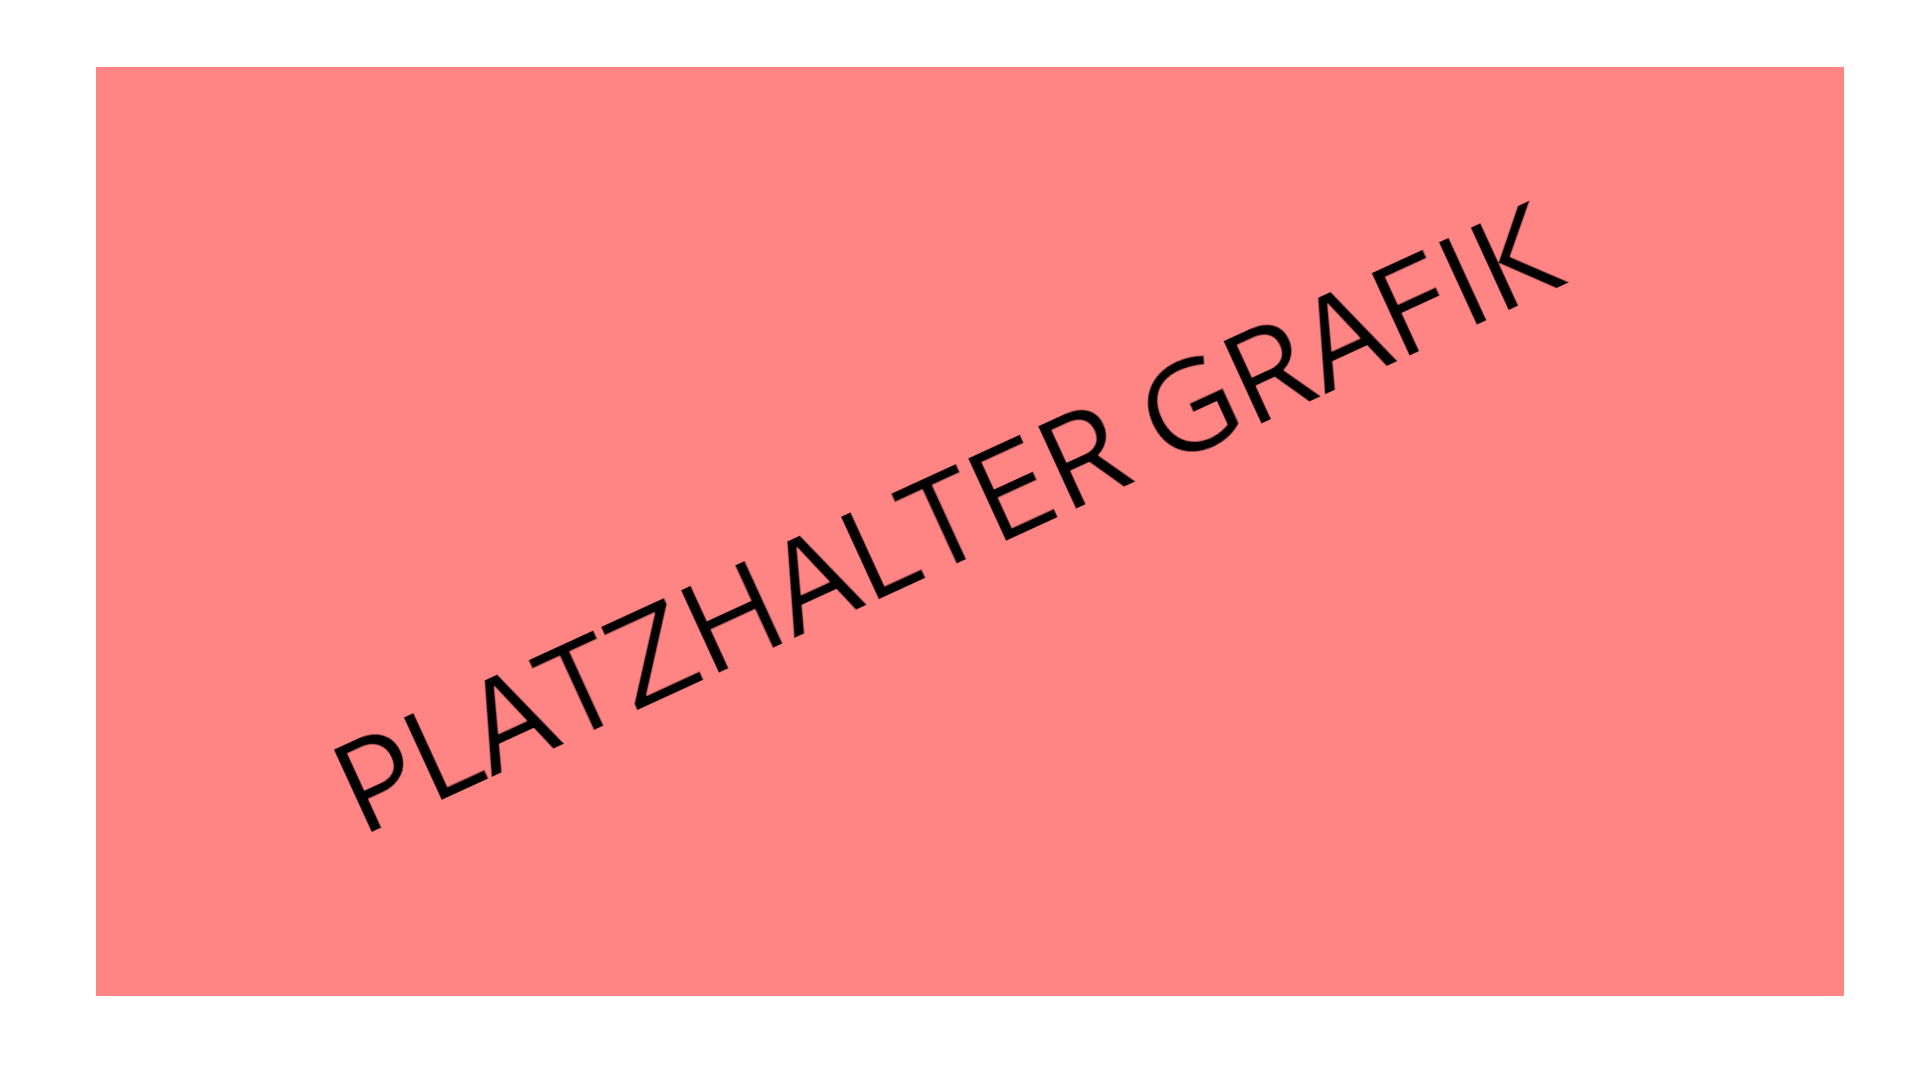
\includegraphics[height=6cm]{bilder/todo.png}
\captionof{figure}{Metamodell - Klassenname}
\end{center}

Lorem ipsum dolor sit amet, consetetur sadipscing elitr, sed diam nonumy eirmod tempor invidunt ut labore et dolore magna aliquyam erat, sed diam voluptua. At vero eos et accusam et justo duo dolores et ea rebum. Stet clita kasd gubergren, no sea takimata sanctus est Lorem ipsum dolor sit amet. Lorem ipsum dolor sit amet, consetetur sadipscing elitr, sed diam nonumy eirmod tempor invidunt ut labore et dolore magna aliquyam erat, sed diam voluptua. At vero eos et accusam et justo duo dolores et ea rebum. Stet clita kasd gubergren, no sea takimata sanctus est Lorem ipsum dolor sit amet. Lorem ipsum dolor sit amet, consetetur sadipscing elitr, sed diam nonumy eirmod tempor invidunt ut labore et dolore magna aliquyam erat, sed diam voluptua. At vero eos et accusam et justo duo dolores et ea rebum. Stet clita kasd gubergren, no sea takimata sanctus est Lorem ipsum dolor sit amet.   

Lorem ipsum dolor sit amet, consetetur sadipscing elitr, sed diam nonumy eirmod tempor invidunt ut labore et dolore magna aliquyam erat, sed diam voluptua. At vero eos et accusam et justo duo dolores et ea rebum. Stet clita kasd gubergren, no sea takimata sanctus est Lorem ipsum dolor sit amet. Lorem ipsum dolor sit amet, consetetur sadipscing elitr, sed diam nonumy eirmod tempor invidunt ut labore et dolore magna aliquyam erat, sed diam voluptua. At vero eos et accusam et justo duo dolores et ea rebum. Stet clita kasd gubergren, no sea takimata sanctus est Lorem ipsum dolor sit amet. Lorem ipsum dolor sit amet, consetetur sadipscing elitr, sed diam nonumy eirmod tempor invidunt ut labore et dolore magna aliquyam erat, sed diam voluptua. At vero eos et accusam et justo duo dolores et ea rebum. Stet clita kasd gubergren, no sea takimata sanctus est Lorem ipsum dolor sit amet.   


\newpage
\paragraph{Logging}

%TODO Grafik machen
\begin{center}
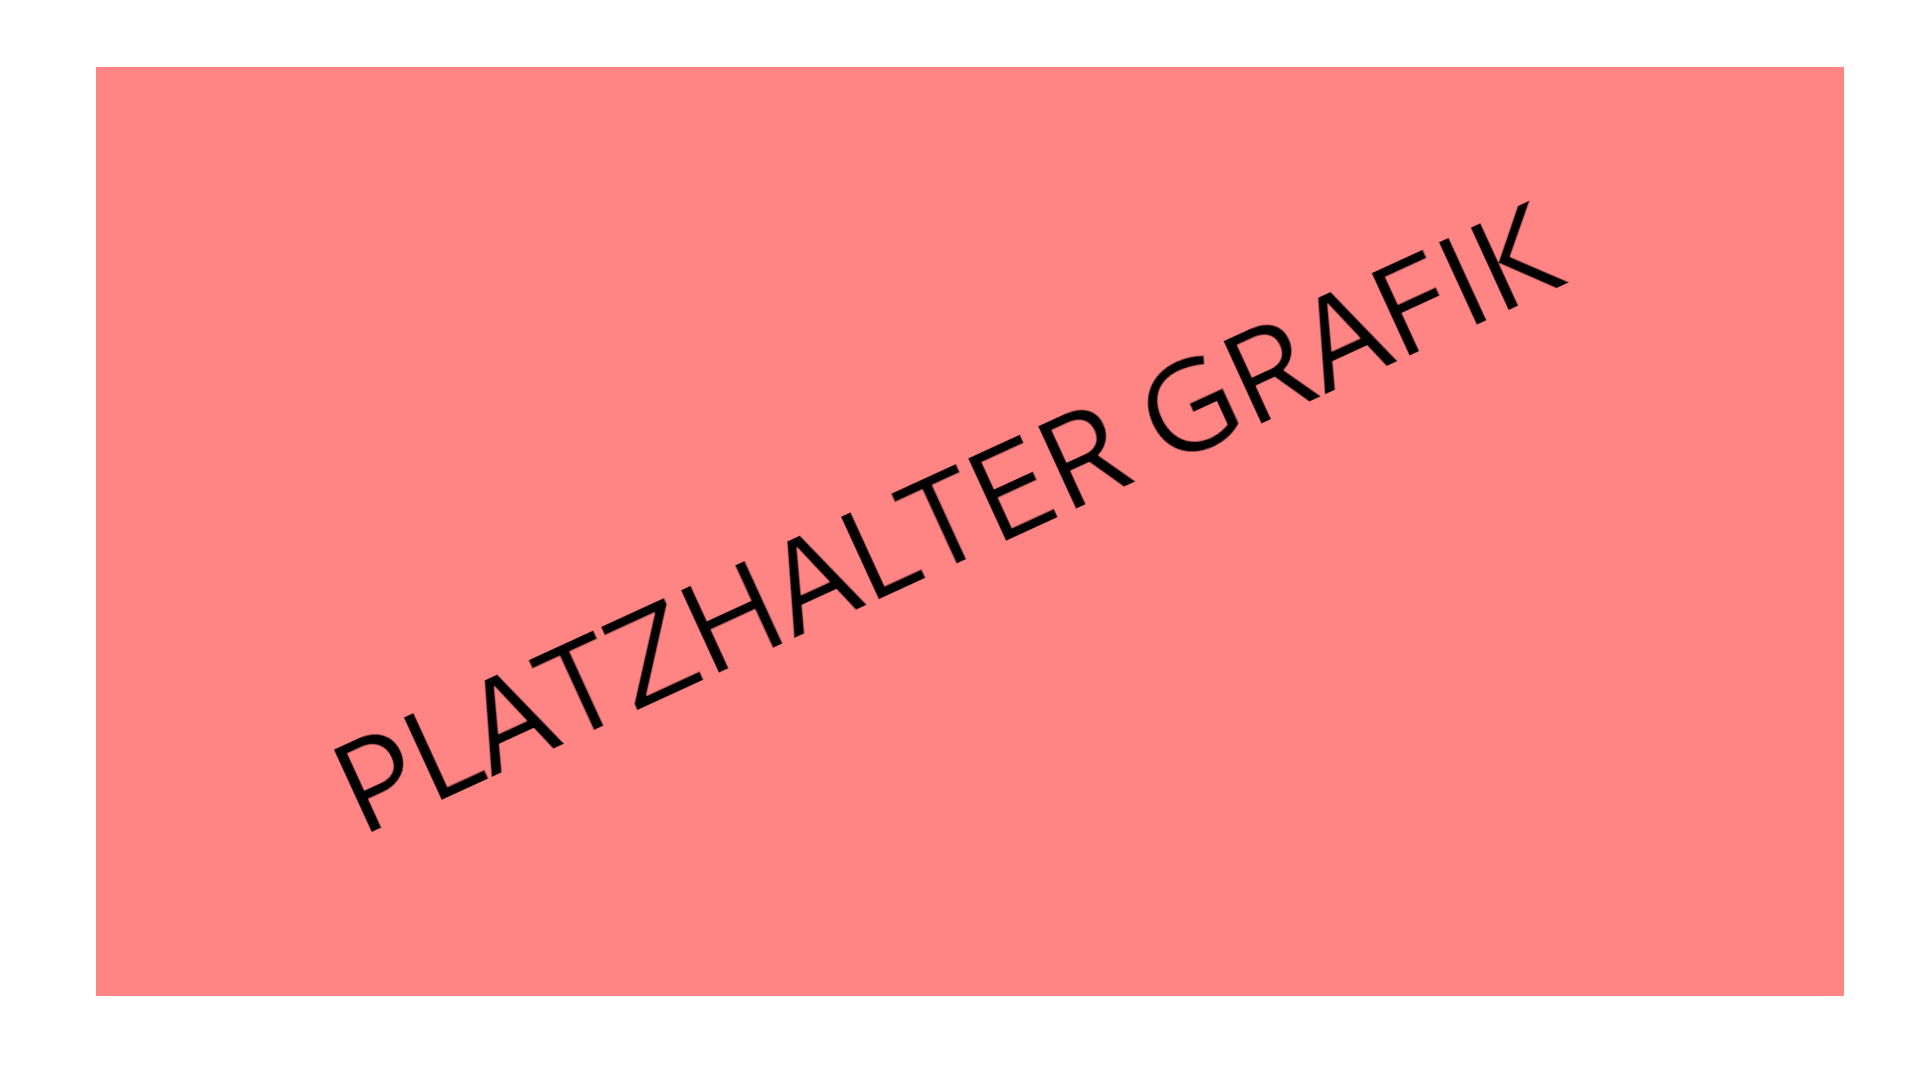
\includegraphics[height=6cm]{bilder/todo.png}
\captionof{figure}{Metamodell - Klassenname}
\end{center}

Lorem ipsum dolor sit amet, consetetur sadipscing elitr, sed diam nonumy eirmod tempor invidunt ut labore et dolore magna aliquyam erat, sed diam voluptua. At vero eos et accusam et justo duo dolores et ea rebum. Stet clita kasd gubergren, no sea takimata sanctus est Lorem ipsum dolor sit amet. Lorem ipsum dolor sit amet, consetetur sadipscing elitr, sed diam nonumy eirmod tempor invidunt ut labore et dolore magna aliquyam erat, sed diam voluptua.

\paragraph{Monitoring}

%TODO Grafik machen
\begin{center}
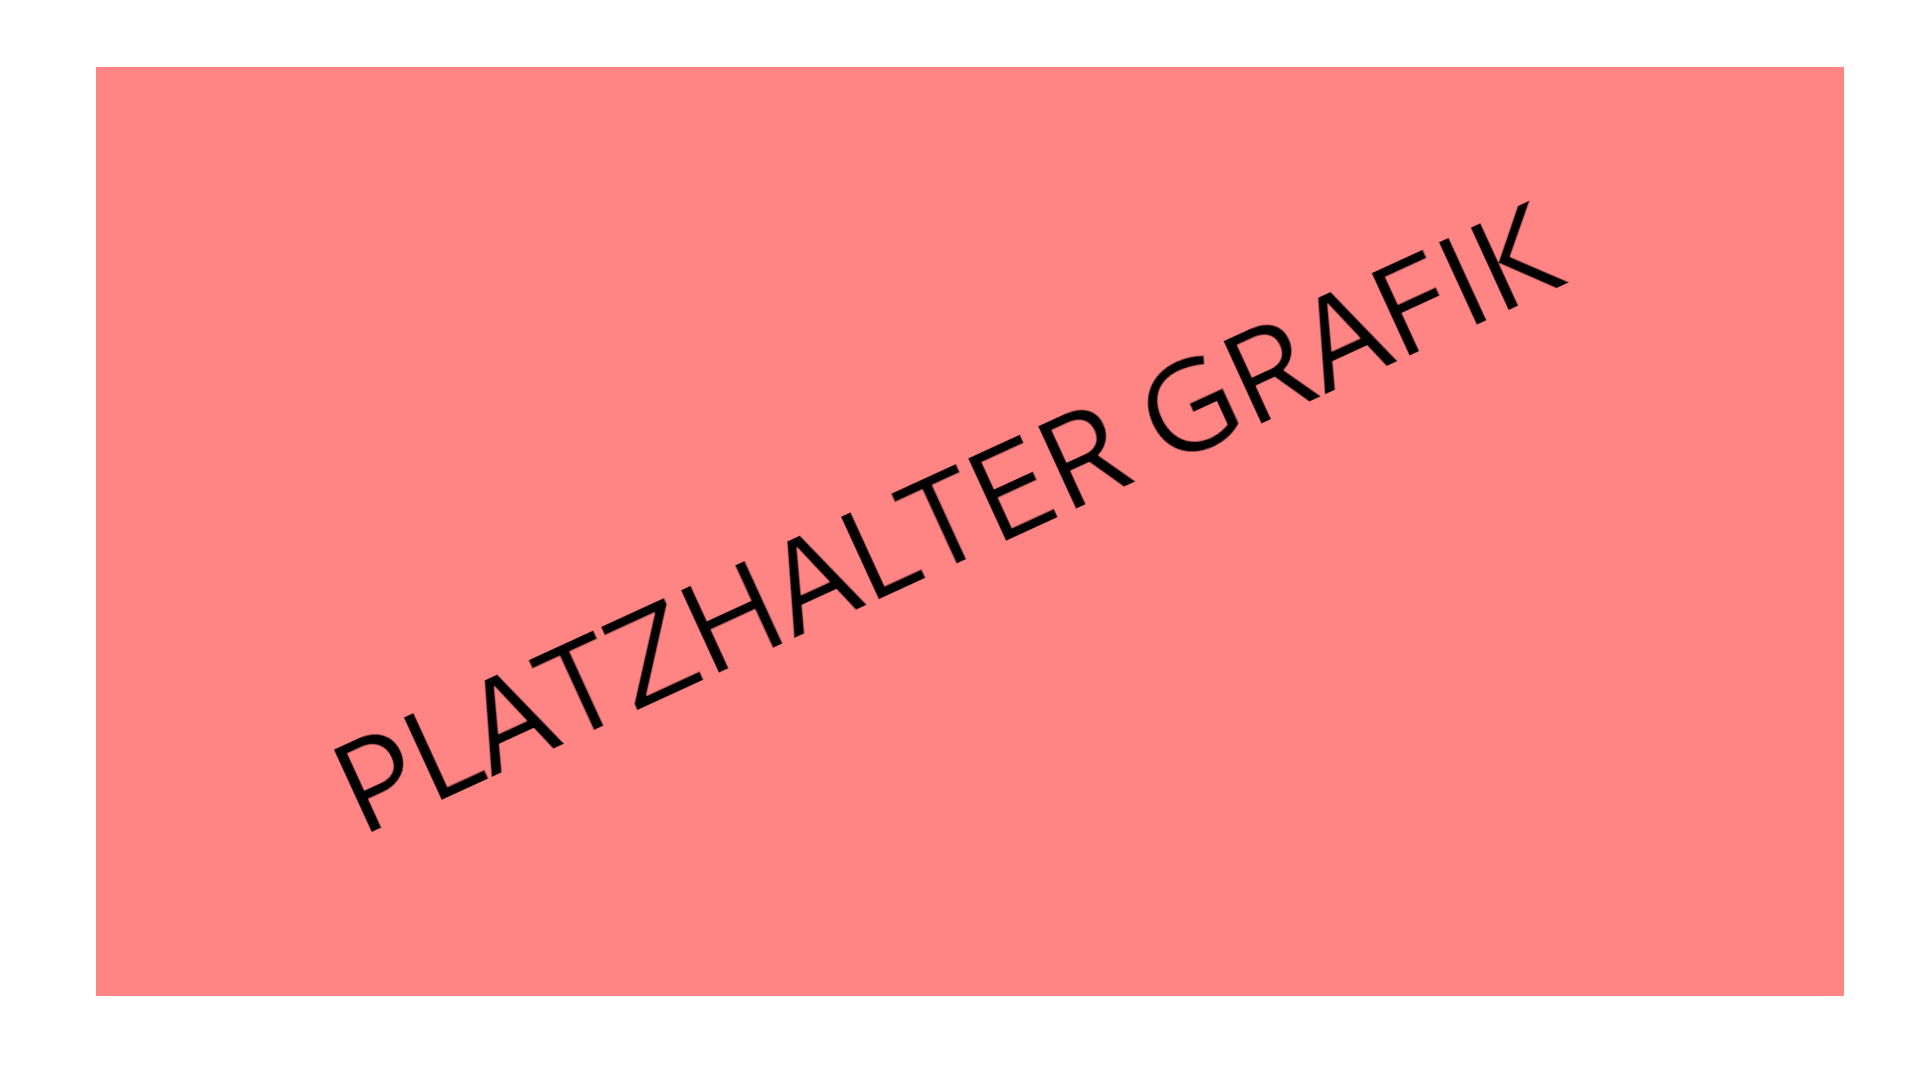
\includegraphics[height=6cm]{bilder/todo.png}
\captionof{figure}{Metamodell - Klassenname}
\end{center}

Lorem ipsum dolor sit amet, consetetur sadipscing elitr, sed diam nonumy eirmod tempor invidunt ut labore et dolore magna aliquyam erat, sed diam voluptua. At vero eos et accusam et justo duo dolores et ea rebum. Stet clita kasd gubergren, no sea takimata sanctus est Lorem ipsum dolor sit amet. Lorem ipsum dolor sit amet, consetetur sadipscing elitr, sed diam nonumy eirmod tempor invidunt ut labore et dolore magna aliquyam erat, sed diam voluptua.

\newpage
\paragraph{Factories}

%TODO Grafik machen
\begin{center}
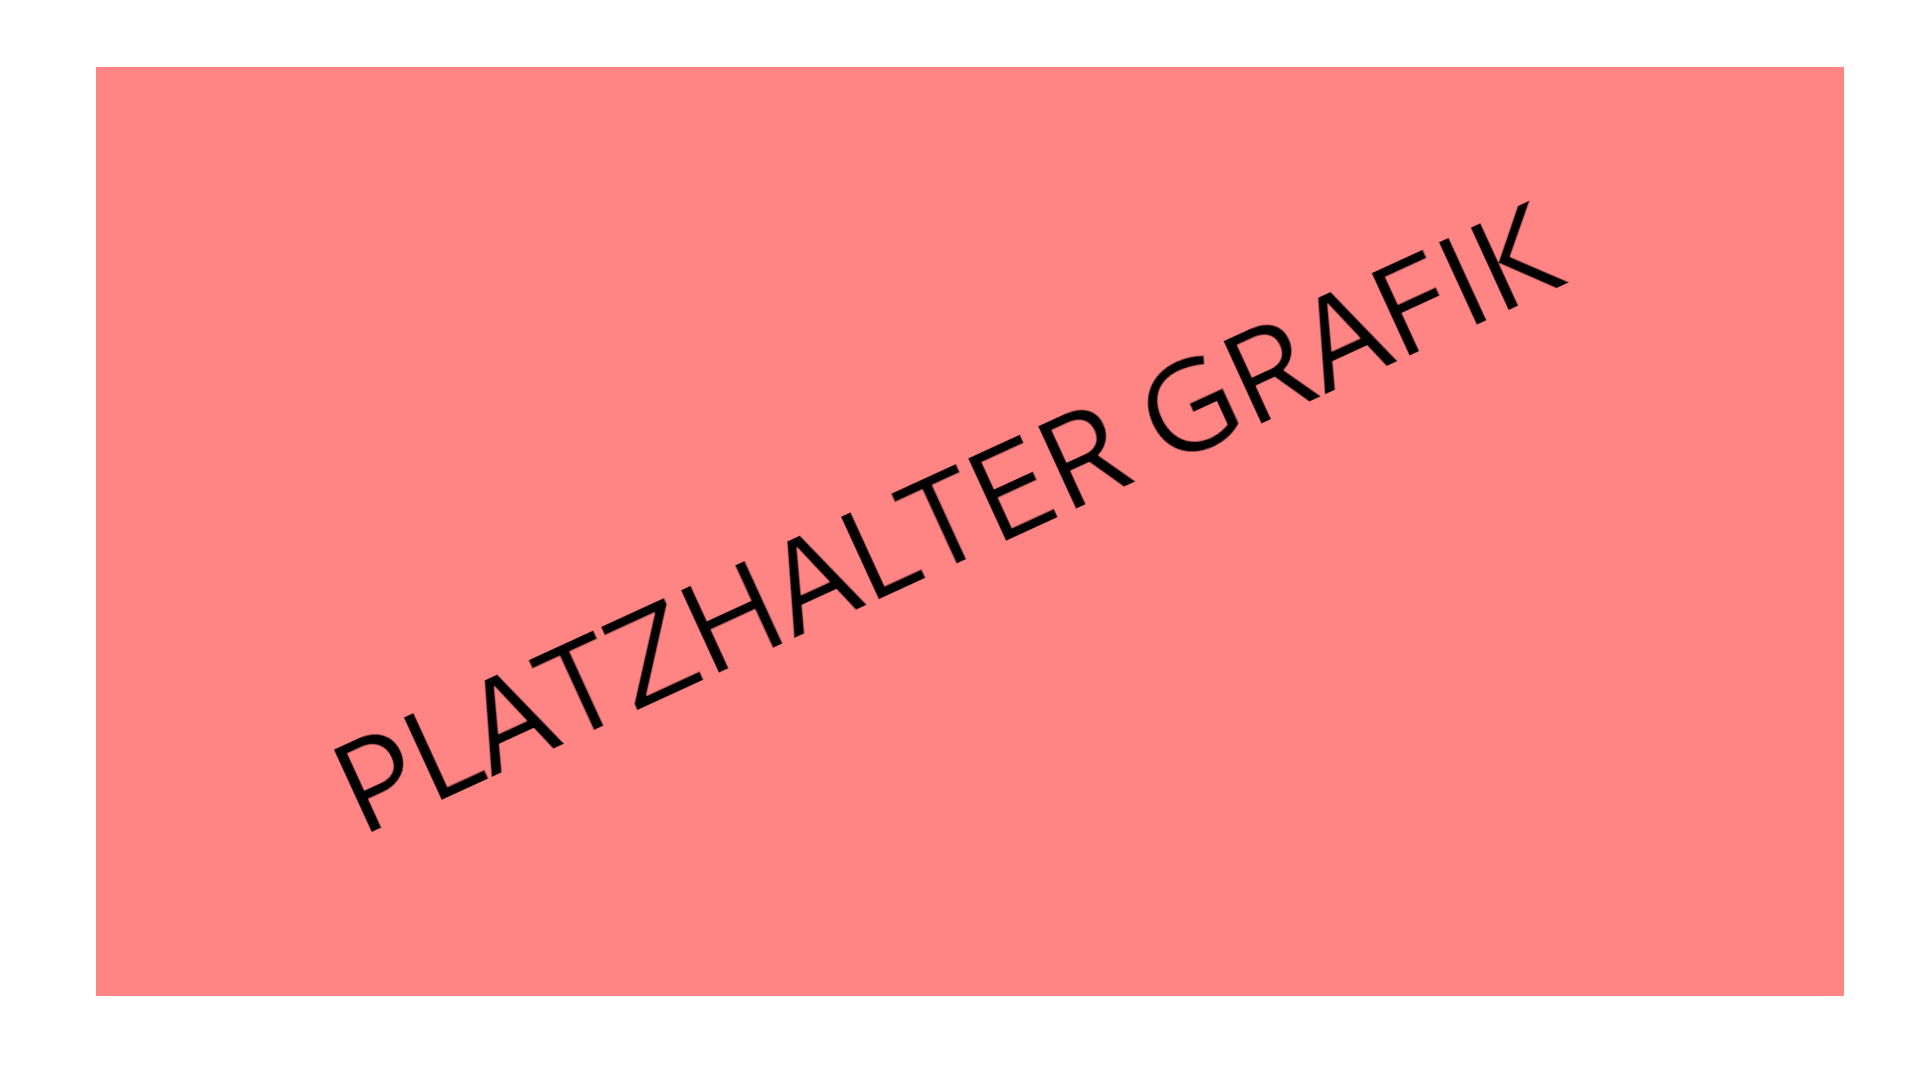
\includegraphics[height=6cm]{bilder/todo.png}
\captionof{figure}{Metamodell - Klassenname}
\end{center}

Lorem ipsum dolor sit amet, consetetur sadipscing elitr, sed diam nonumy eirmod tempor invidunt ut labore et dolore magna aliquyam erat, sed diam voluptua. At vero eos et accusam et justo duo dolores et ea rebum. Stet clita kasd gubergren, no sea takimata sanctus est Lorem ipsum dolor sit amet. Lorem ipsum dolor sit amet, consetetur sadipscing elitr, sed diam nonumy eirmod tempor invidunt ut labore et dolore magna aliquyam erat, sed diam voluptua.

\newpage
\paragraph{Gesamtüberblick}

\begin{center}
\rotatebox{90}{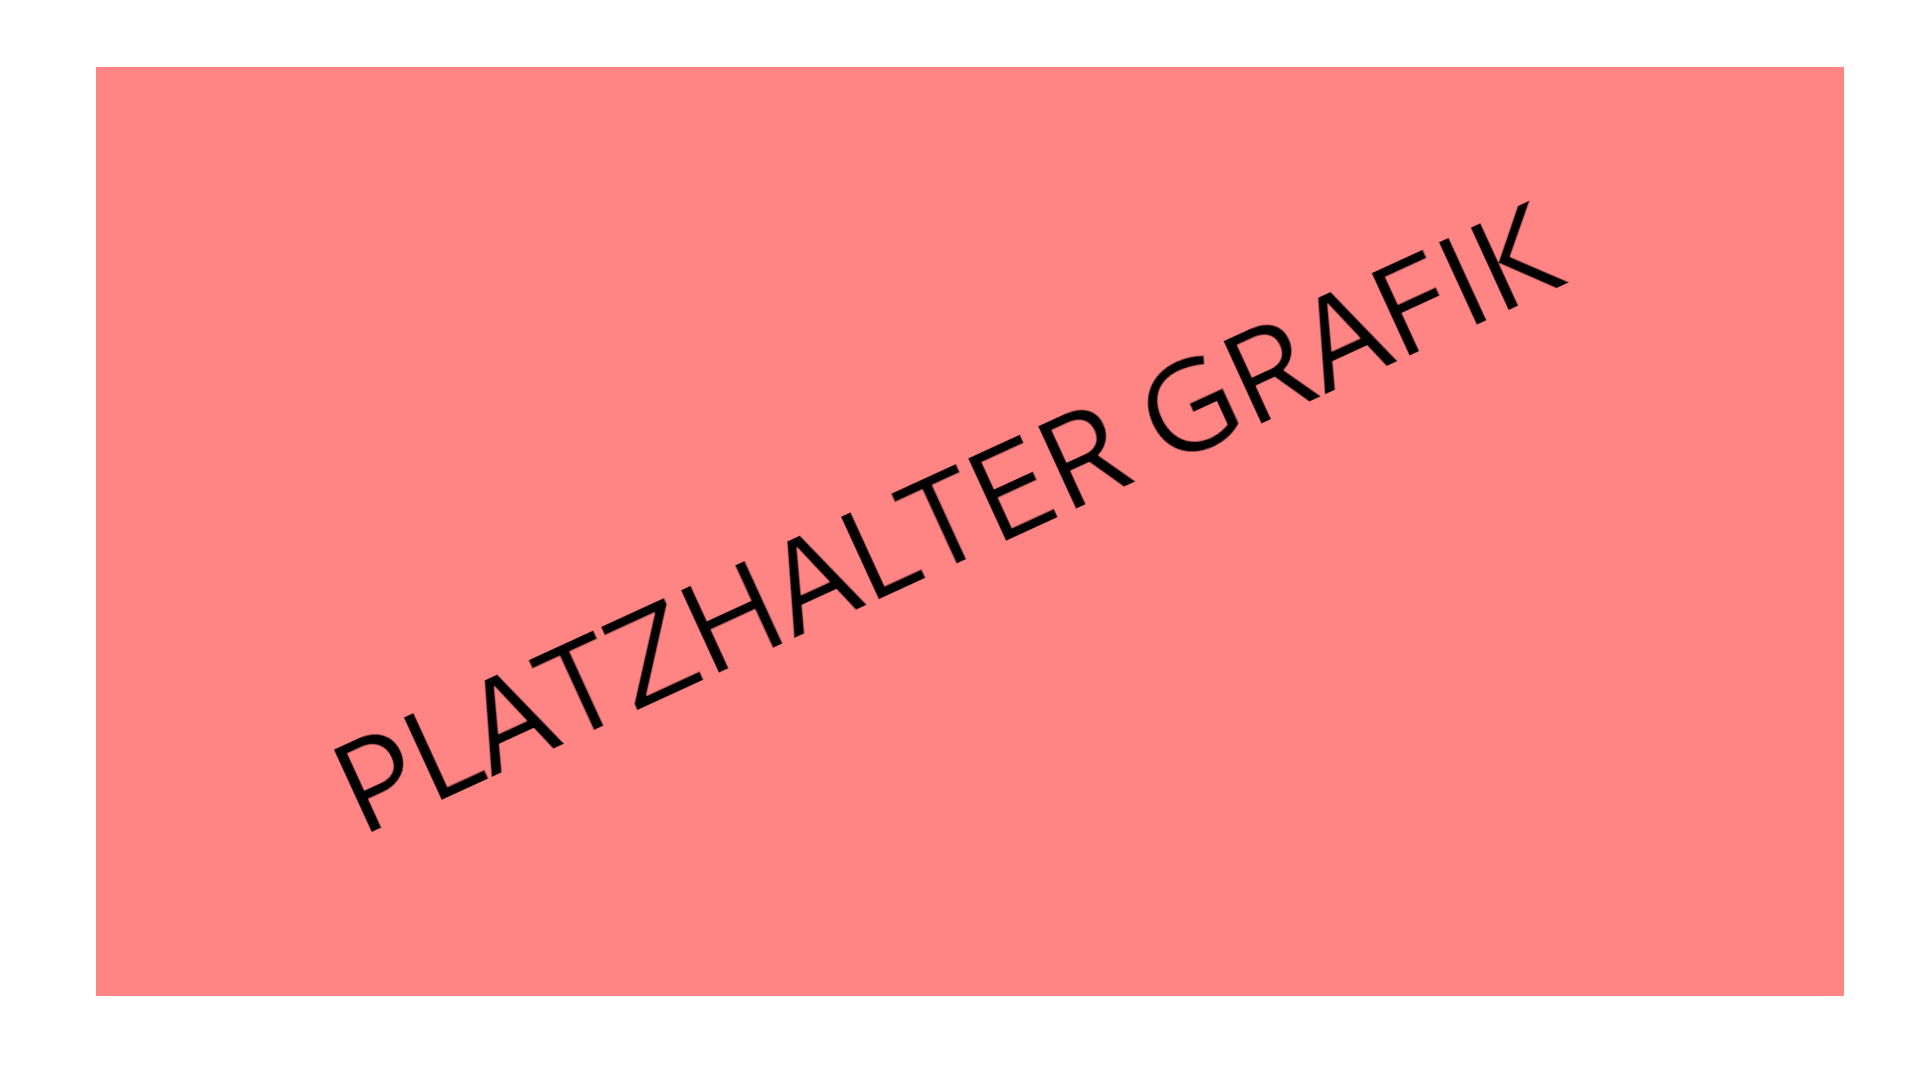
\includegraphics[height=10cm]{bilder/todo.png}}
\captionof{figure}{Metamodell - Klassenname}
\end{center}

%%%%%%%%%%%%%%%%%%%%%%%%%%%%%%%%%%%%%%%%%%%%%%%%%%%%%%%%%%%%%%%%%%%%%%%%%%%%%%%%%%%%%%%%%%%%%%%%%%%%%%%%%%%%%%%%%%%%
%			Abbildung Fachl -> Techn.
%%%%%%%%%%%%%%%%%%%%%%%%%%%%%%%%%%%%%%%%%%%%%%%%%%%%%%%%%%%%%%%%%%%%%%%%%%%%%%%%%%%%%%%%%%%%%%%%%%%%%%%%%%%%%%%%%%%%

\newpage
\subsubsection{Abbildung der fachlichen Schicht auf eine Technische Schicht}

\paragraph{Schicht}

%TODO Grafik machen
\begin{center}
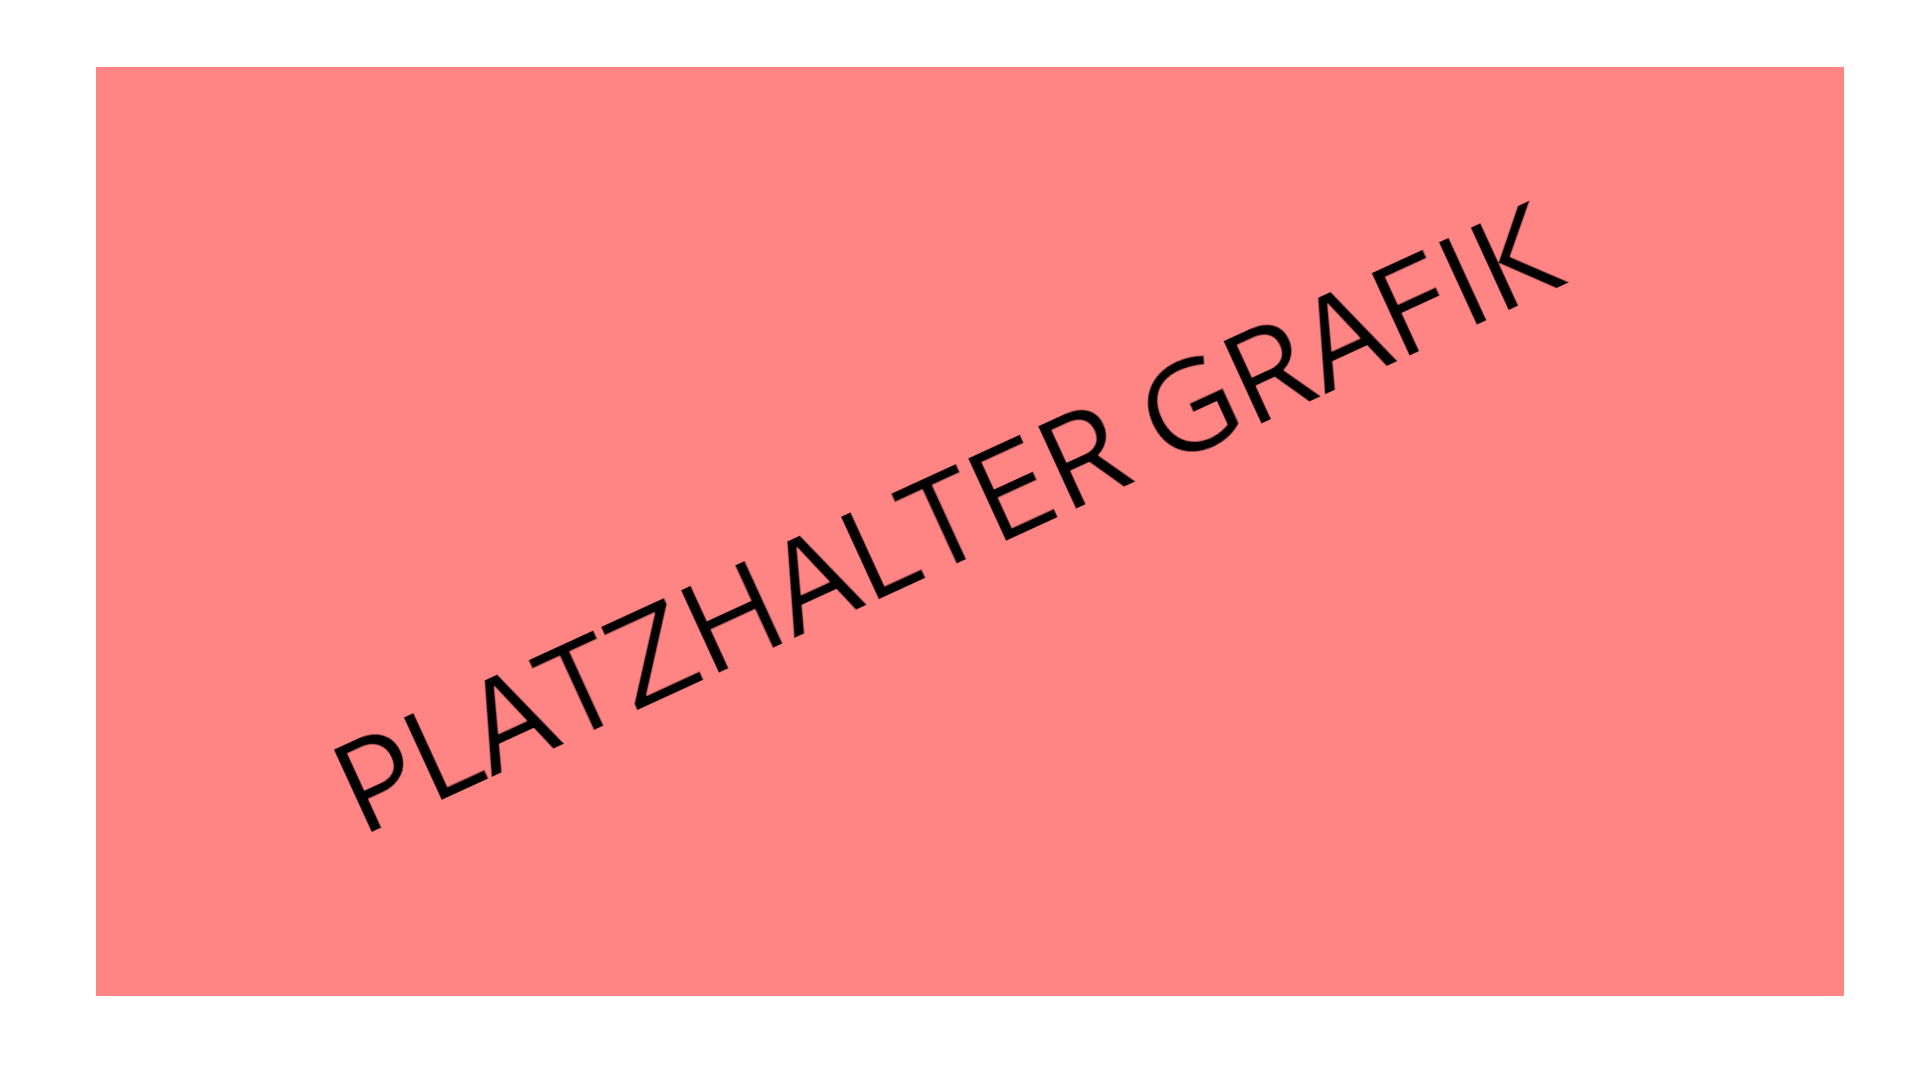
\includegraphics[height=6cm]{bilder/todo.png}
\captionof{figure}{Metamodell - Klassenname}
\end{center}

Lorem ipsum dolor sit amet, consetetur sadipscing elitr, sed diam nonumy eirmod tempor invidunt ut labore et dolore magna aliquyam erat, sed diam voluptua. At vero eos et accusam et justo duo dolores et ea rebum. Stet clita kasd gubergren, no sea takimata sanctus est Lorem ipsum dolor sit amet. Lorem ipsum dolor sit amet, consetetur sadipscing elitr, sed diam nonumy eirmod tempor invidunt ut labore et dolore magna aliquyam erat, sed diam voluptua.

\paragraph{Paket}

%TODO Grafik machen
\begin{center}
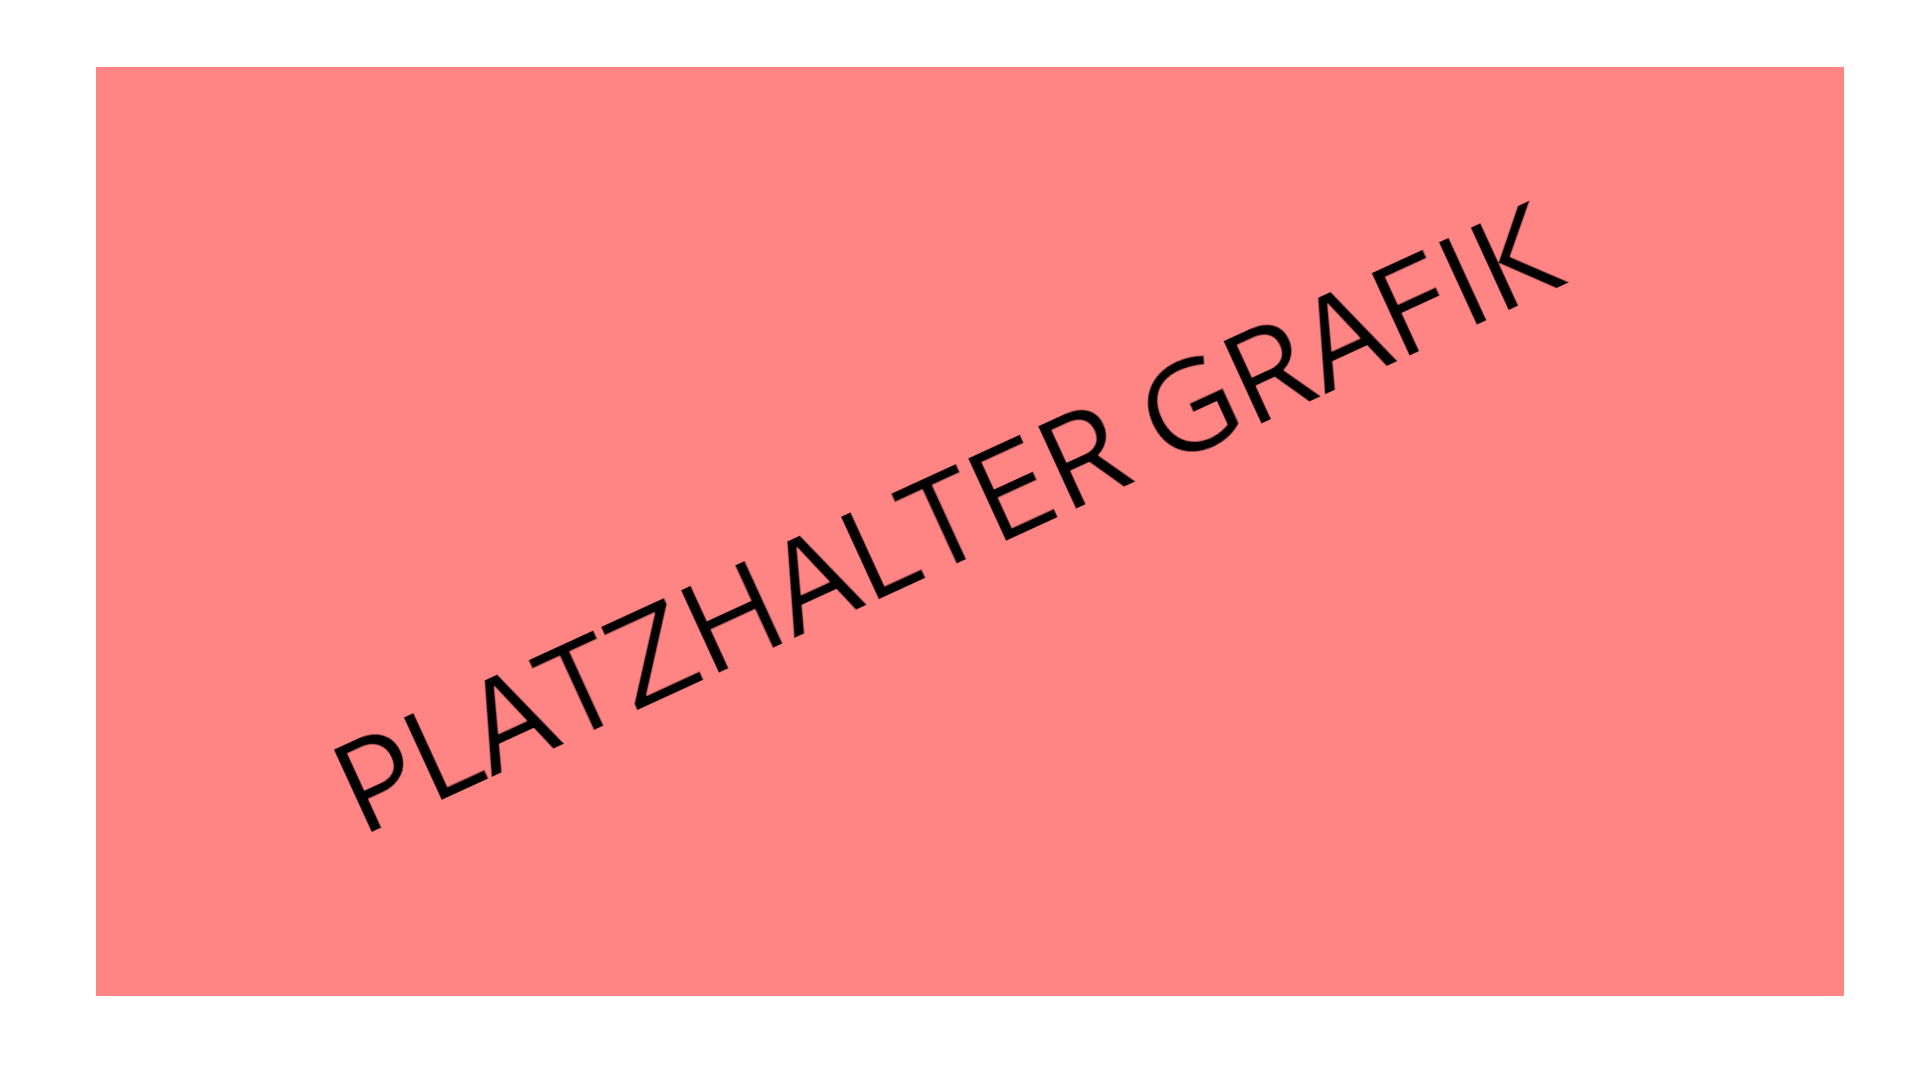
\includegraphics[height=6cm]{bilder/todo.png}
\captionof{figure}{Metamodell - Klassenname}
\end{center}

Lorem ipsum dolor sit amet, consetetur sadipscing elitr, sed diam nonumy eirmod tempor invidunt ut labore et dolore magna aliquyam erat, sed diam voluptua. At vero eos et accusam et justo duo dolores et ea rebum. Stet clita kasd gubergren, no sea takimata sanctus est Lorem ipsum dolor sit amet. Lorem ipsum dolor sit amet, consetetur sadipscing elitr, sed diam nonumy eirmod tempor invidunt ut labore et dolore magna aliquyam erat, sed diam voluptua.

\newpage
\paragraph{Entitiy}

%TODO Grafik machen
\begin{center}
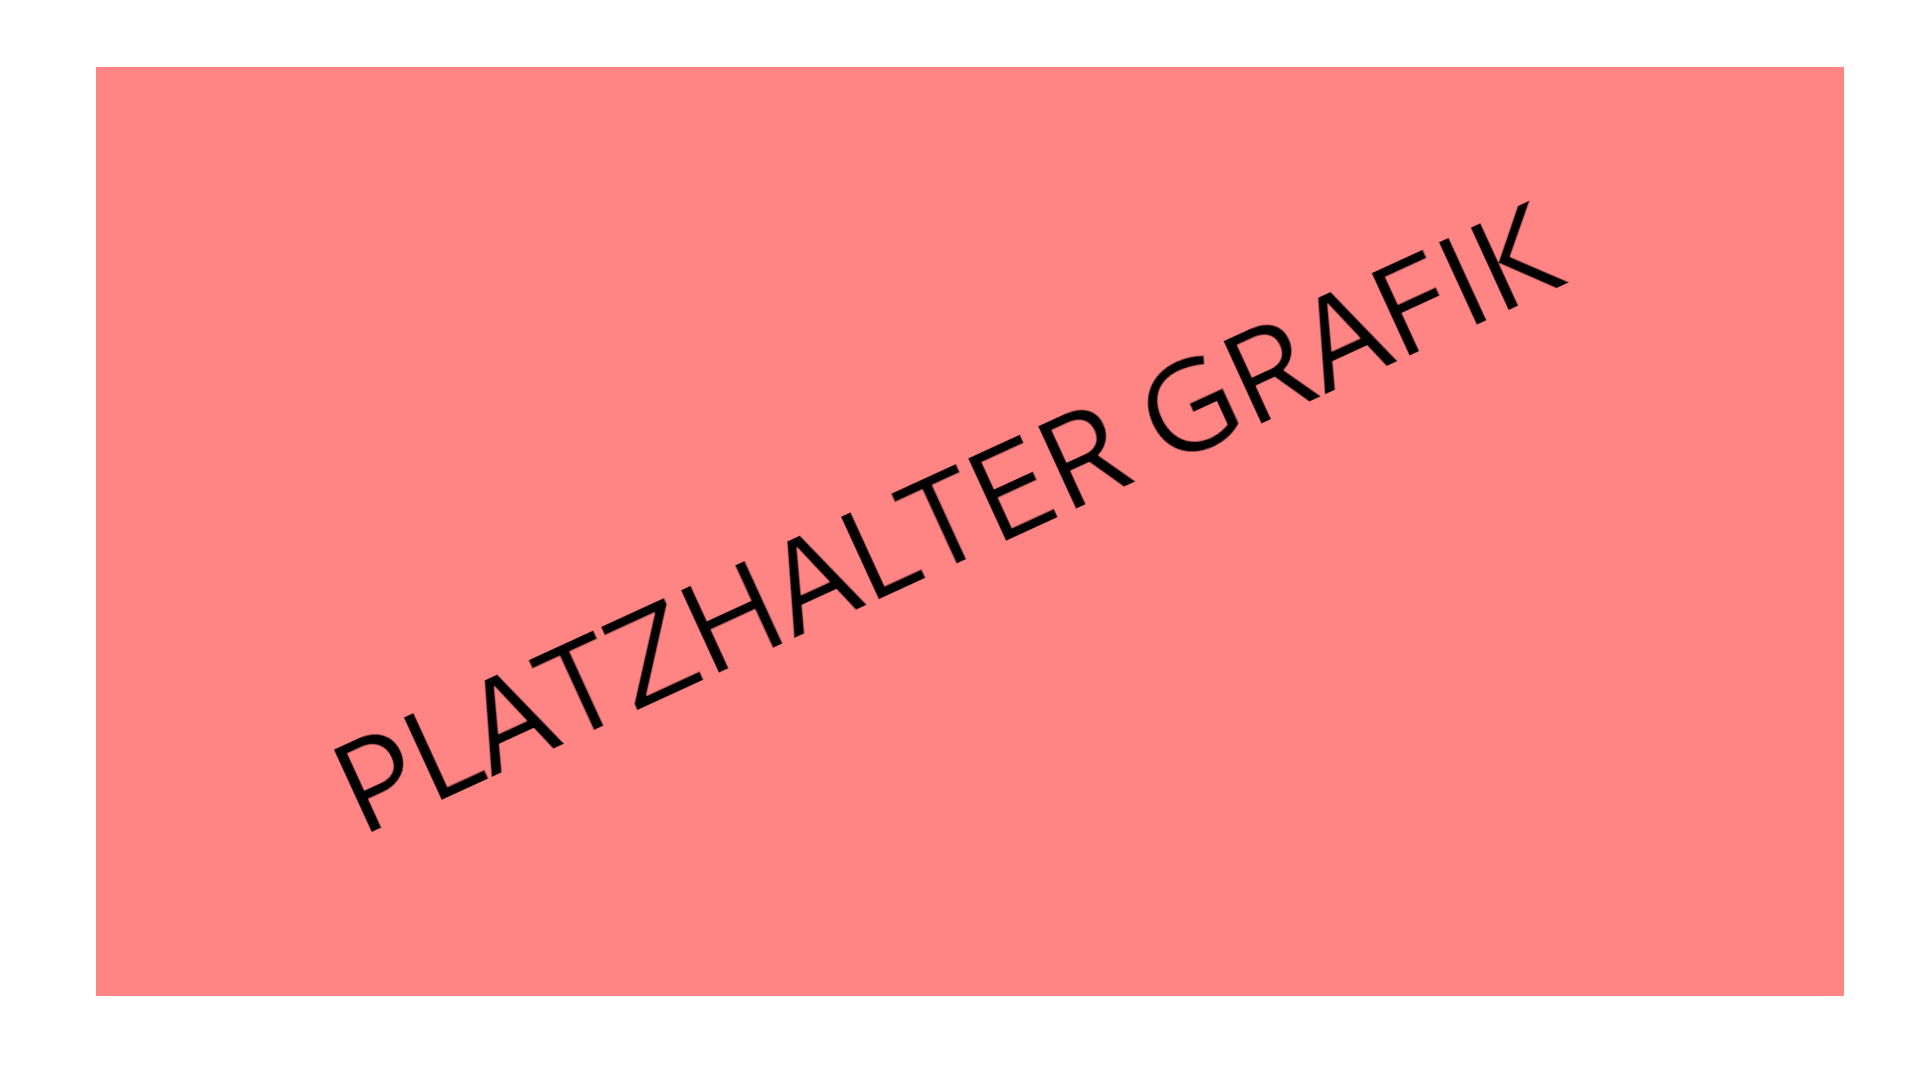
\includegraphics[height=6cm]{bilder/todo.png}
\captionof{figure}{Metamodell - Klassenname}
\end{center}

Lorem ipsum dolor sit amet, consetetur sadipscing elitr, sed diam nonumy eirmod tempor invidunt ut labore et dolore magna aliquyam erat, sed diam voluptua. At vero eos et accusam et justo duo dolores et ea rebum. Stet clita kasd gubergren, no sea takimata sanctus est Lorem ipsum dolor sit amet. Lorem ipsum dolor sit amet, consetetur sadipscing elitr, sed diam nonumy eirmod tempor invidunt ut labore et dolore magna aliquyam erat, sed diam voluptua.

\paragraph{Value Object}

%TODO Grafik machen
\begin{center}
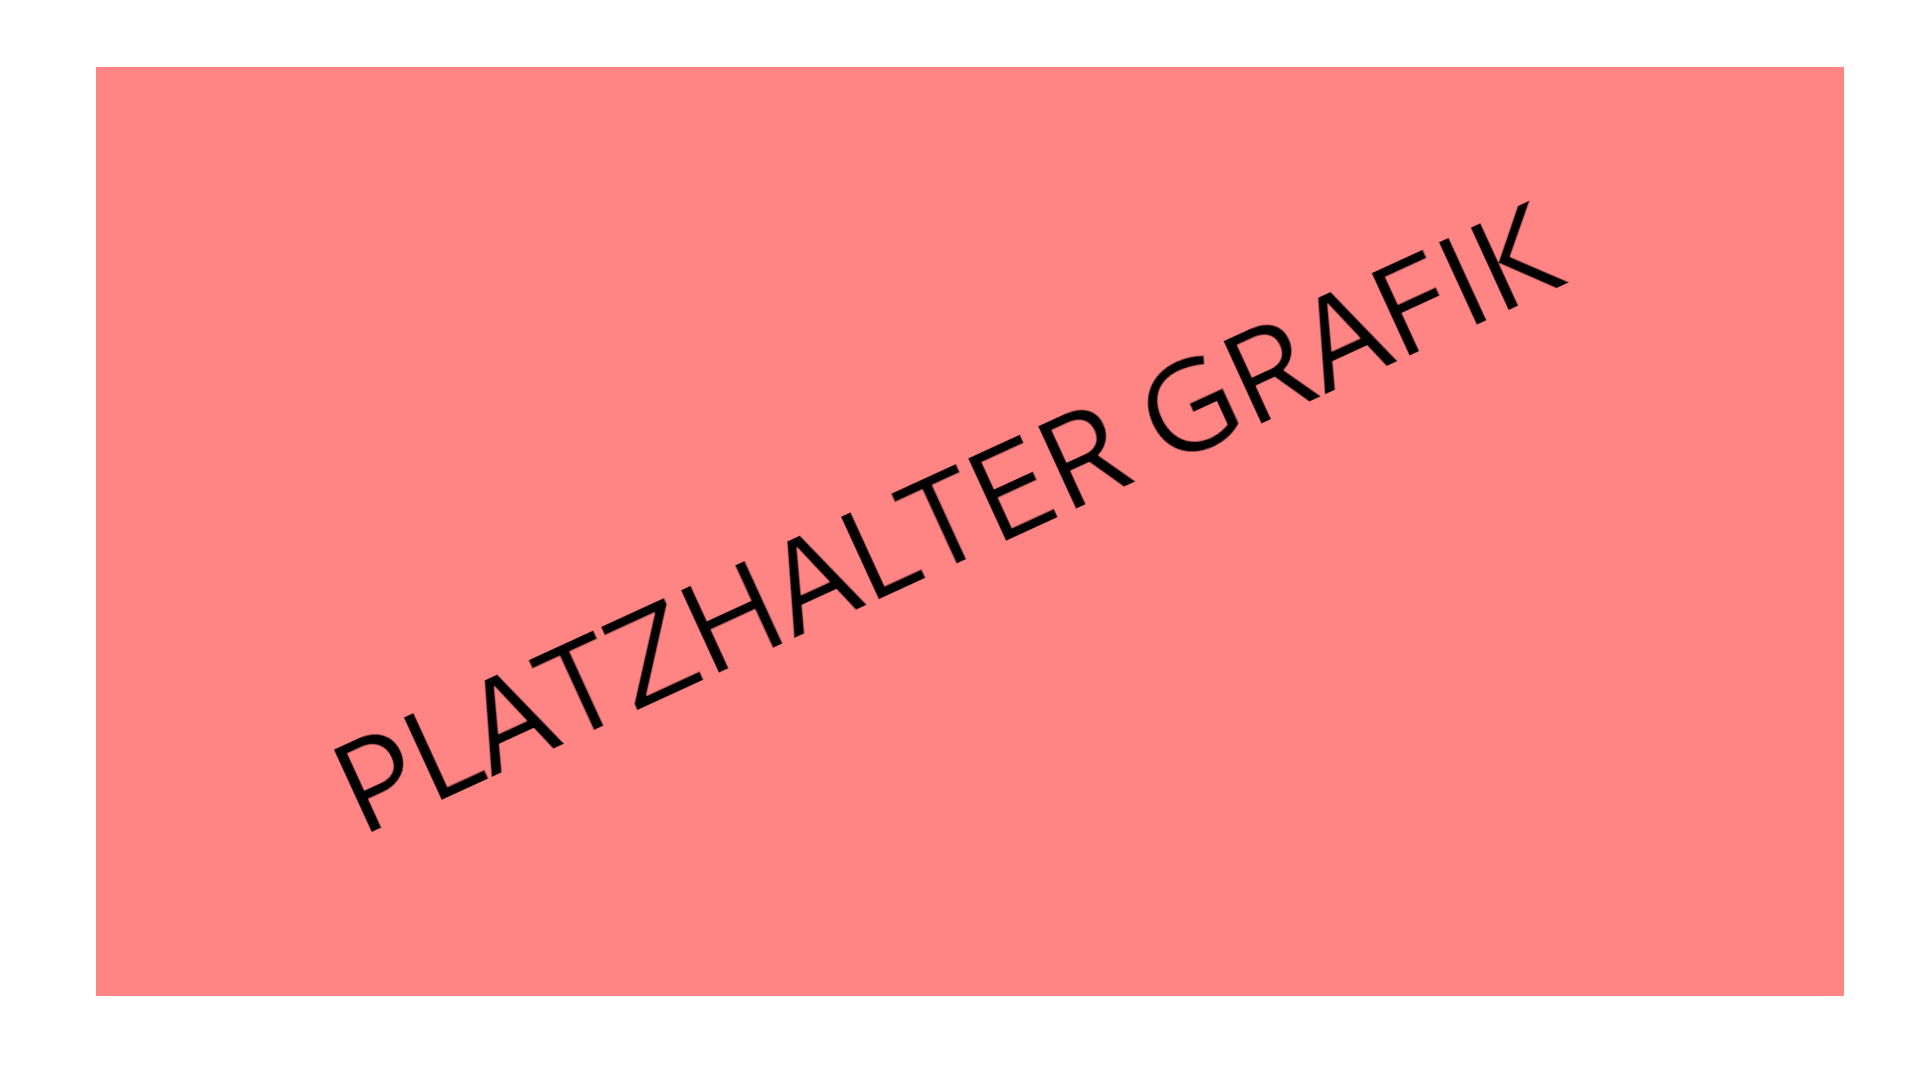
\includegraphics[height=6cm]{bilder/todo.png}
\captionof{figure}{Metamodell - Klassenname}
\end{center}

Lorem ipsum dolor sit amet, consetetur sadipscing elitr, sed diam nonumy eirmod tempor invidunt ut labore et dolore magna aliquyam erat, sed diam voluptua. At vero eos et accusam et justo duo dolores et ea rebum. Stet clita kasd gubergren, no sea takimata sanctus est Lorem ipsum dolor sit amet. Lorem ipsum dolor sit amet, consetetur sadipscing elitr, sed diam nonumy eirmod tempor invidunt ut labore et dolore magna aliquyam erat, sed diam voluptua.

\newpage
\paragraph{Service}

%TODO Grafik machen
\begin{center}
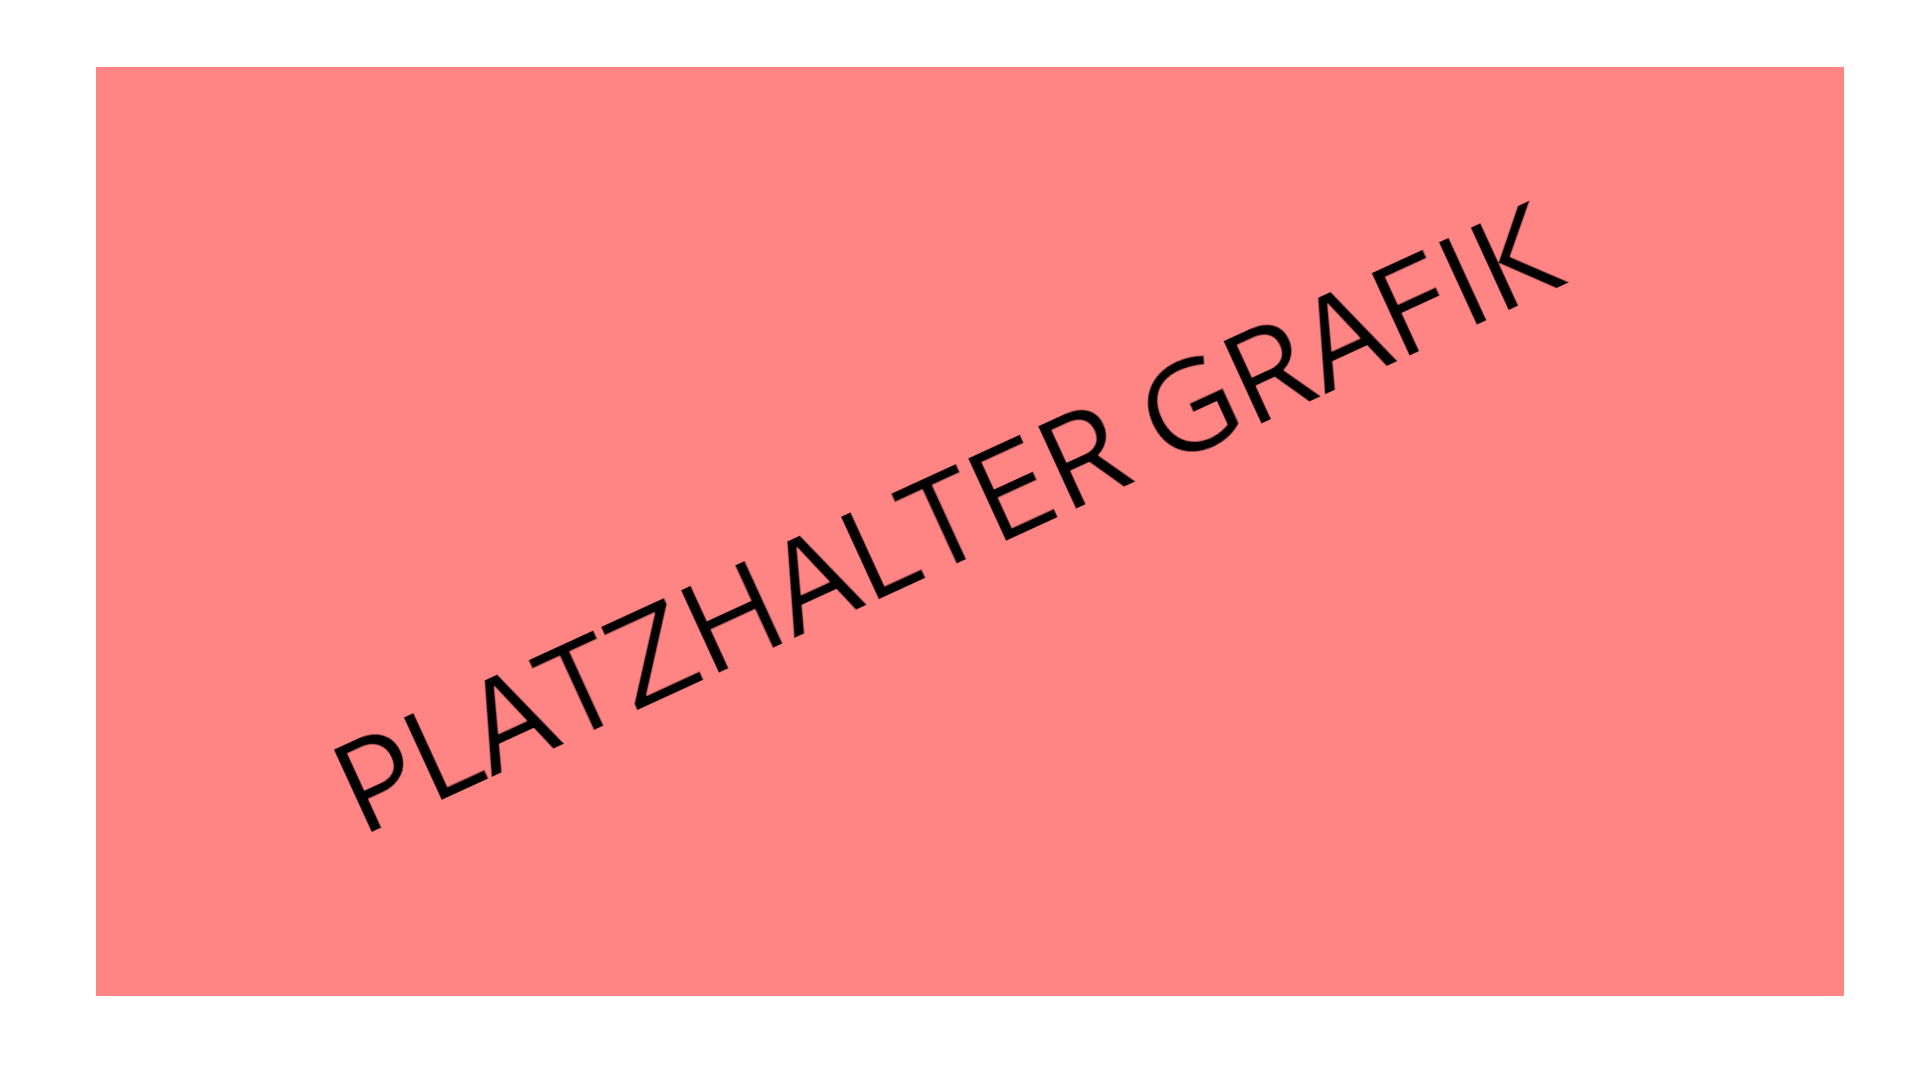
\includegraphics[height=6cm]{bilder/todo.png}
\captionof{figure}{Metamodell - Klassenname}
\end{center}

Lorem ipsum dolor sit amet, consetetur sadipscing elitr, sed diam nonumy eirmod tempor invidunt ut labore et dolore magna aliquyam erat, sed diam voluptua. At vero eos et accusam et justo duo dolores et ea rebum. Stet clita kasd gubergren, no sea takimata sanctus est Lorem ipsum dolor sit amet. Lorem ipsum dolor sit amet, consetetur sadipscing elitr, sed diam nonumy eirmod tempor invidunt ut labore et dolore magna aliquyam erat, sed diam voluptua.

\paragraph{Aggregate}

%TODO Grafik machen
\begin{center}
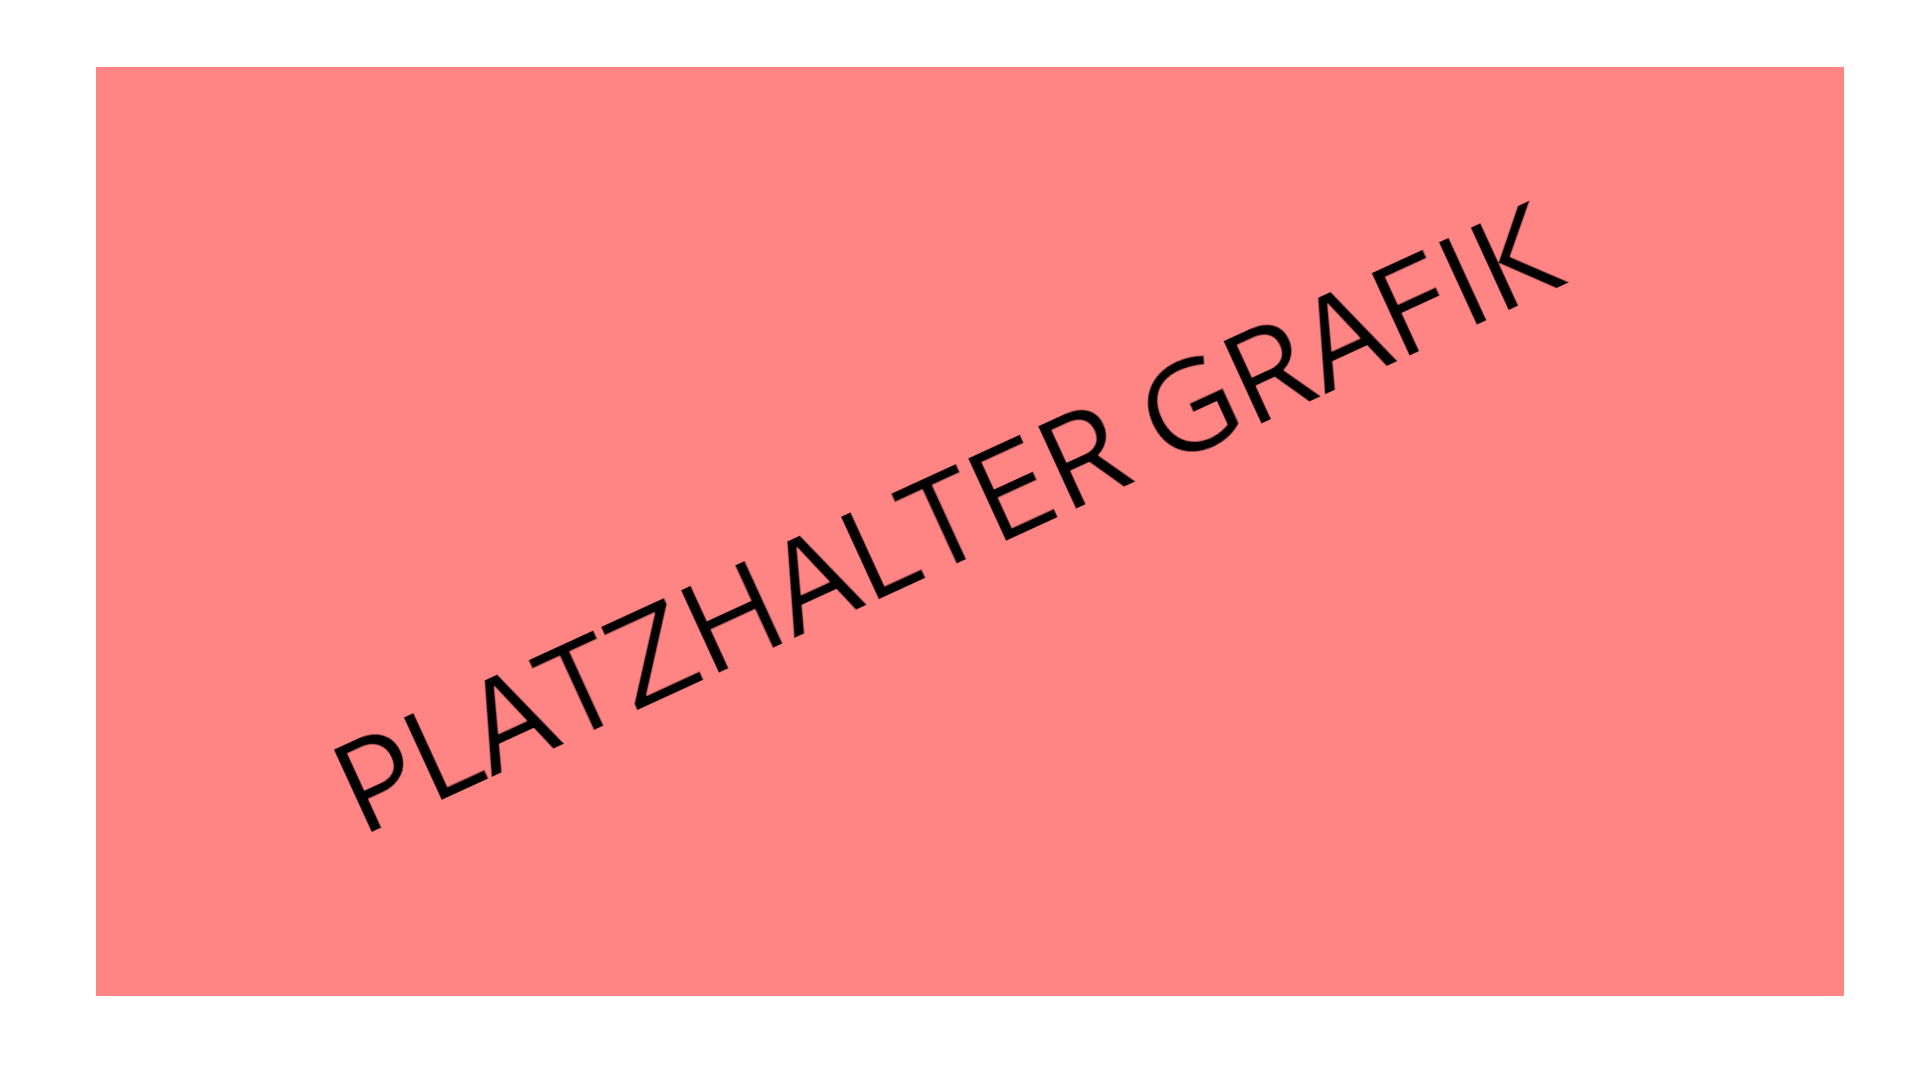
\includegraphics[height=6cm]{bilder/todo.png}
\captionof{figure}{Metamodell - Klassenname}
\end{center}

Lorem ipsum dolor sit amet, consetetur sadipscing elitr, sed diam nonumy eirmod tempor invidunt ut labore et dolore magna aliquyam erat, sed diam voluptua. At vero eos et accusam et justo duo dolores et ea rebum. Stet clita kasd gubergren, no sea takimata sanctus est Lorem ipsum dolor sit amet. Lorem ipsum dolor sit amet, consetetur sadipscing elitr, sed diam nonumy eirmod tempor invidunt ut labore et dolore magna aliquyam erat, sed diam voluptua.

\newpage
\paragraph{Factory}

%TODO Grafik machen
\begin{center}
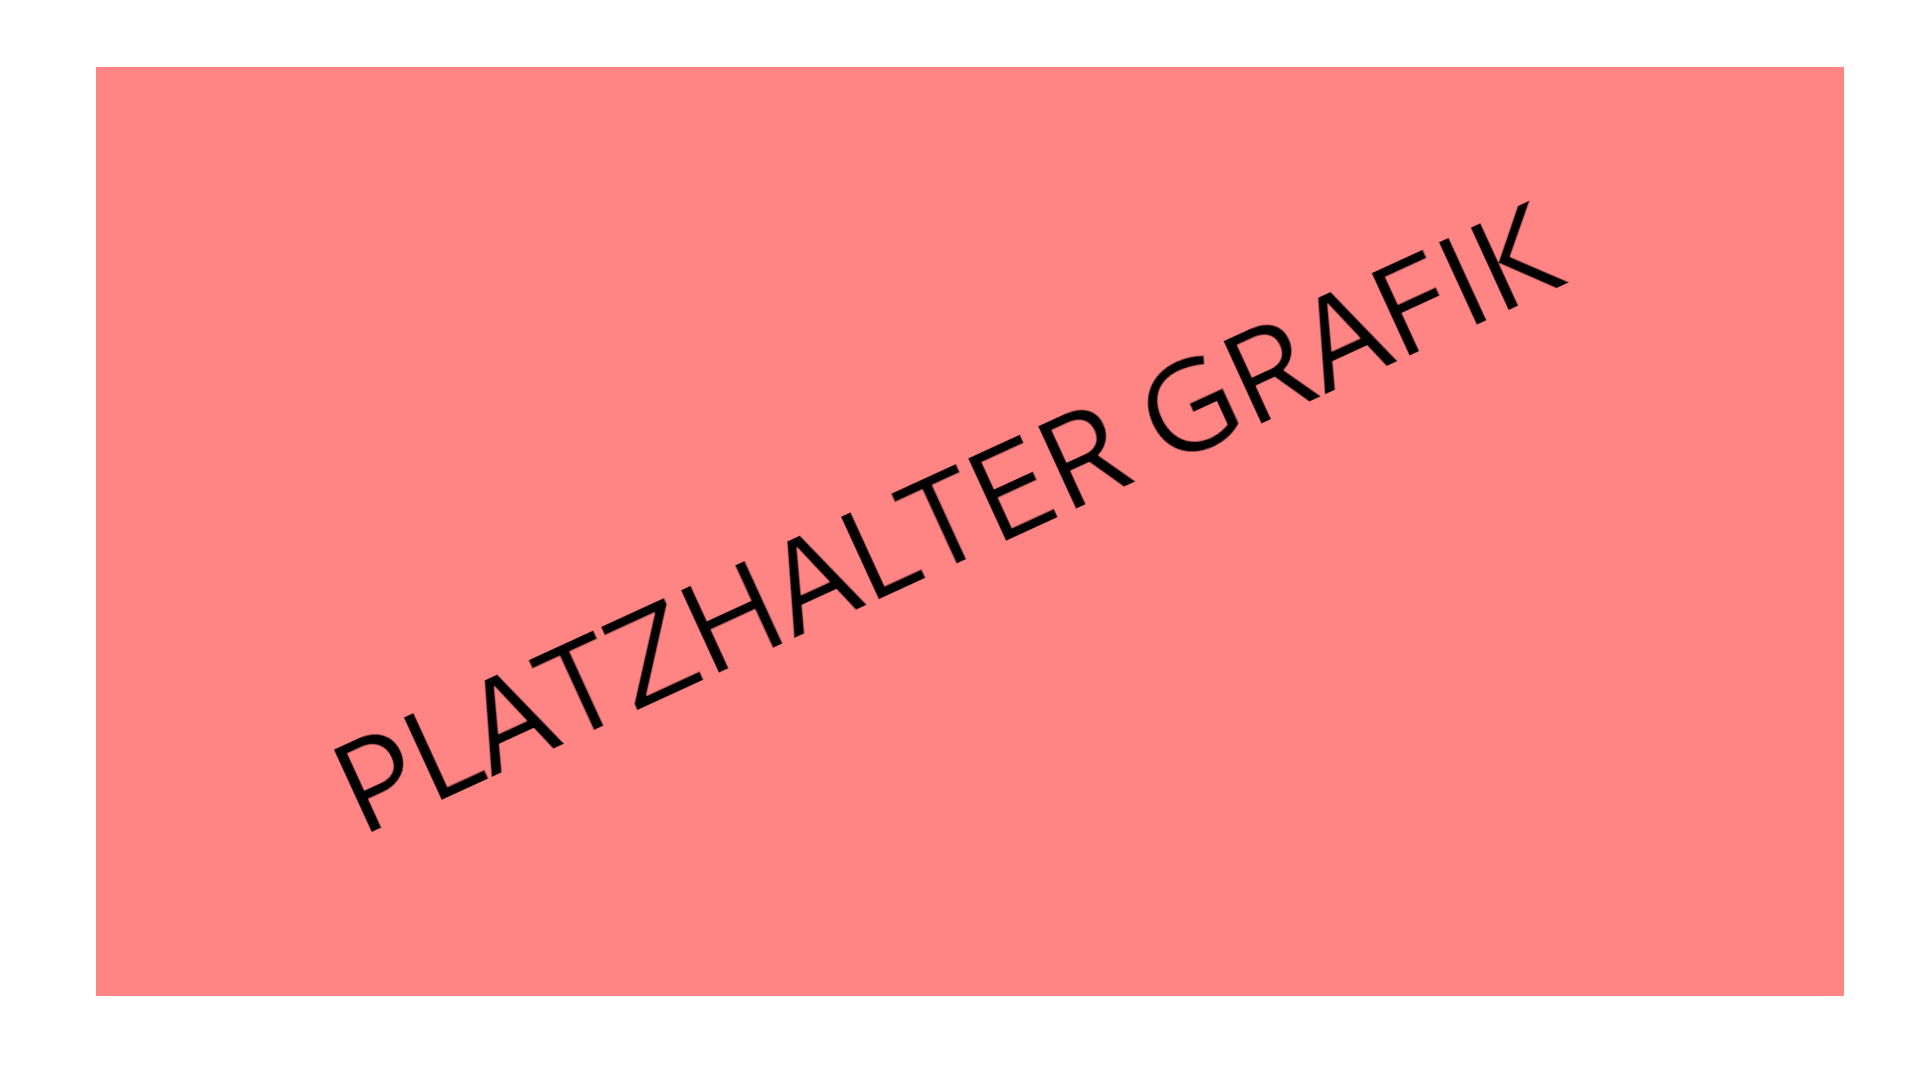
\includegraphics[height=6cm]{bilder/todo.png}
\captionof{figure}{Metamodell - Klassenname}
\end{center}

Lorem ipsum dolor sit amet, consetetur sadipscing elitr, sed diam nonumy eirmod tempor invidunt ut labore et dolore magna aliquyam erat, sed diam voluptua. At vero eos et accusam et justo duo dolores et ea rebum. Stet clita kasd gubergren, no sea takimata sanctus est Lorem ipsum dolor sit amet. Lorem ipsum dolor sit amet, consetetur sadipscing elitr, sed diam nonumy eirmod tempor invidunt ut labore et dolore magna aliquyam erat, sed diam voluptua.

\paragraph{Repository}

%TODO Grafik machen
\begin{center}
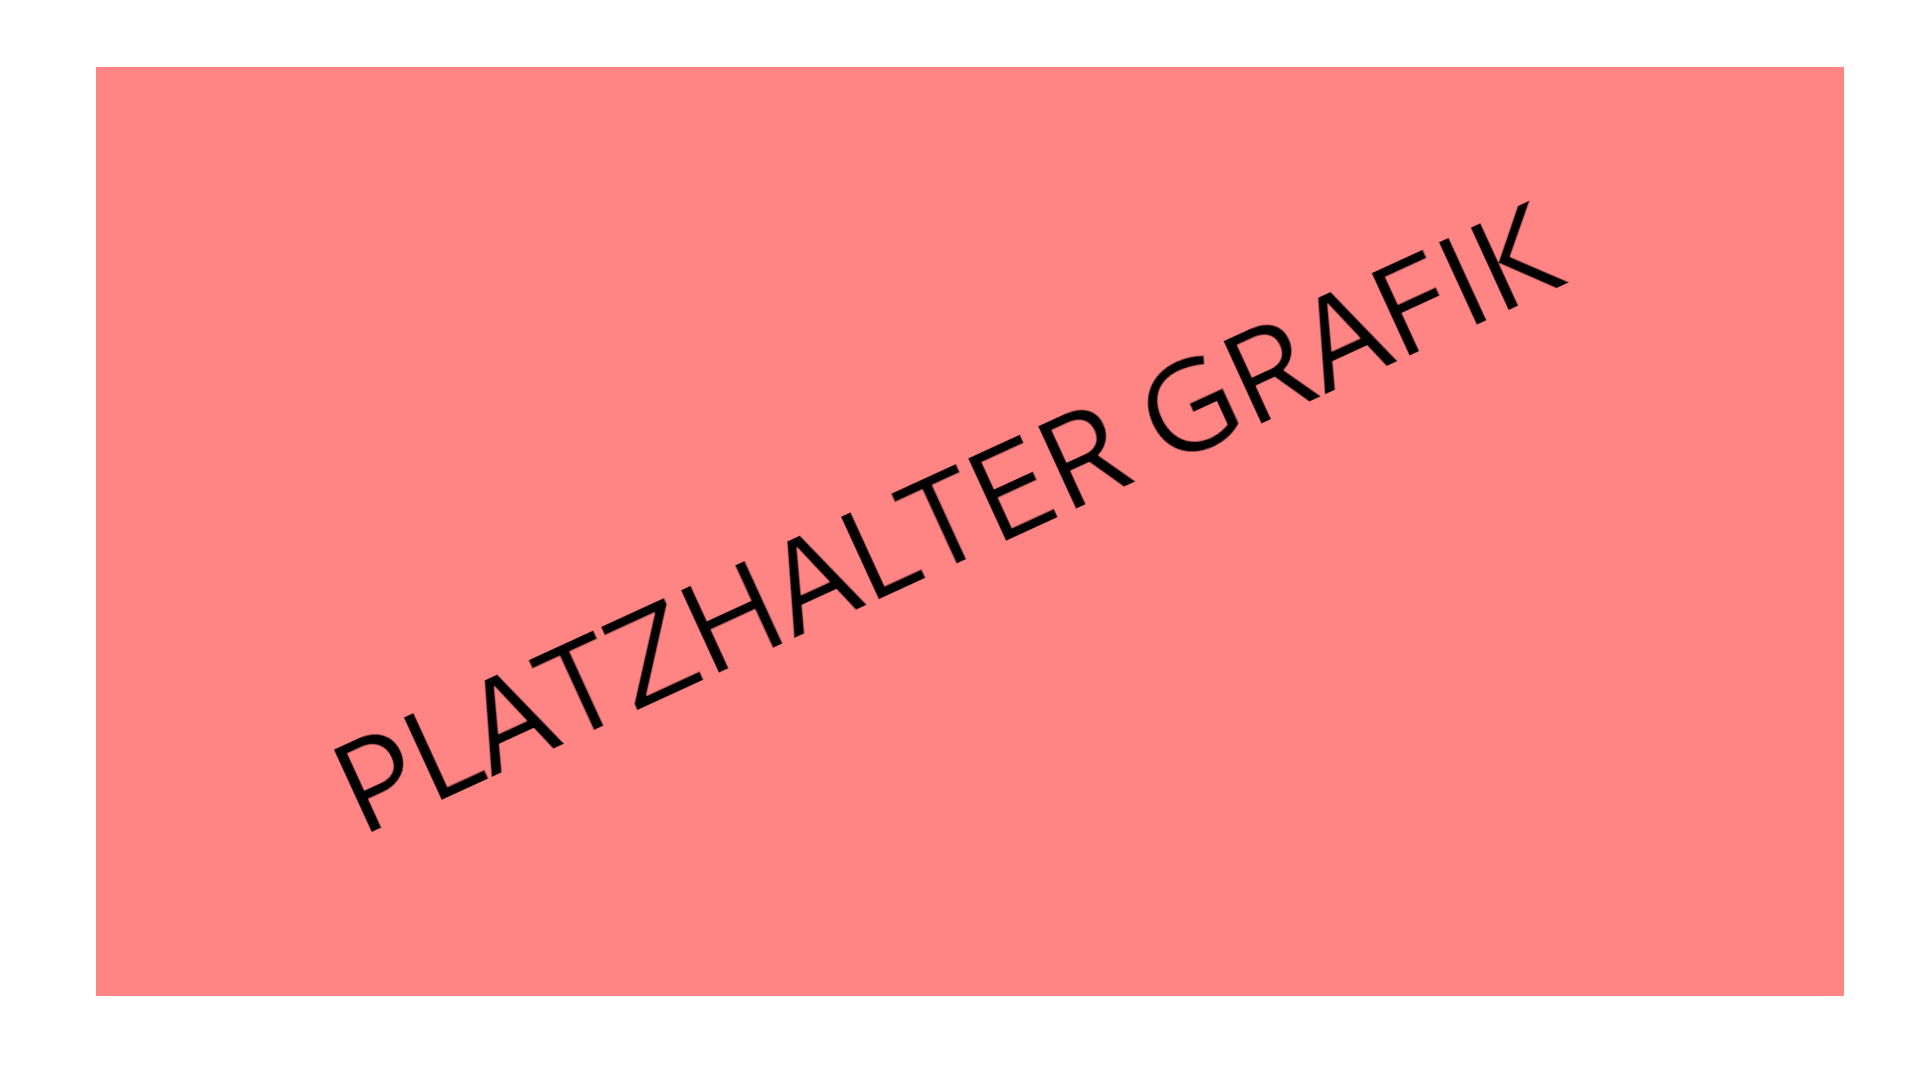
\includegraphics[height=6cm]{bilder/todo.png}
\captionof{figure}{Metamodell - Klassenname}
\end{center}

Lorem ipsum dolor sit amet, consetetur sadipscing elitr, sed diam nonumy eirmod tempor invidunt ut labore et dolore magna aliquyam erat, sed diam voluptua. At vero eos et accusam et justo duo dolores et ea rebum. Stet clita kasd gubergren, no sea takimata sanctus est Lorem ipsum dolor sit amet. Lorem ipsum dolor sit amet, consetetur sadipscing elitr, sed diam nonumy eirmod tempor invidunt ut labore et dolore magna aliquyam erat, sed diam voluptua.

\newpage
\paragraph{Bounded Context}

%TODO Grafik machen
\begin{center}
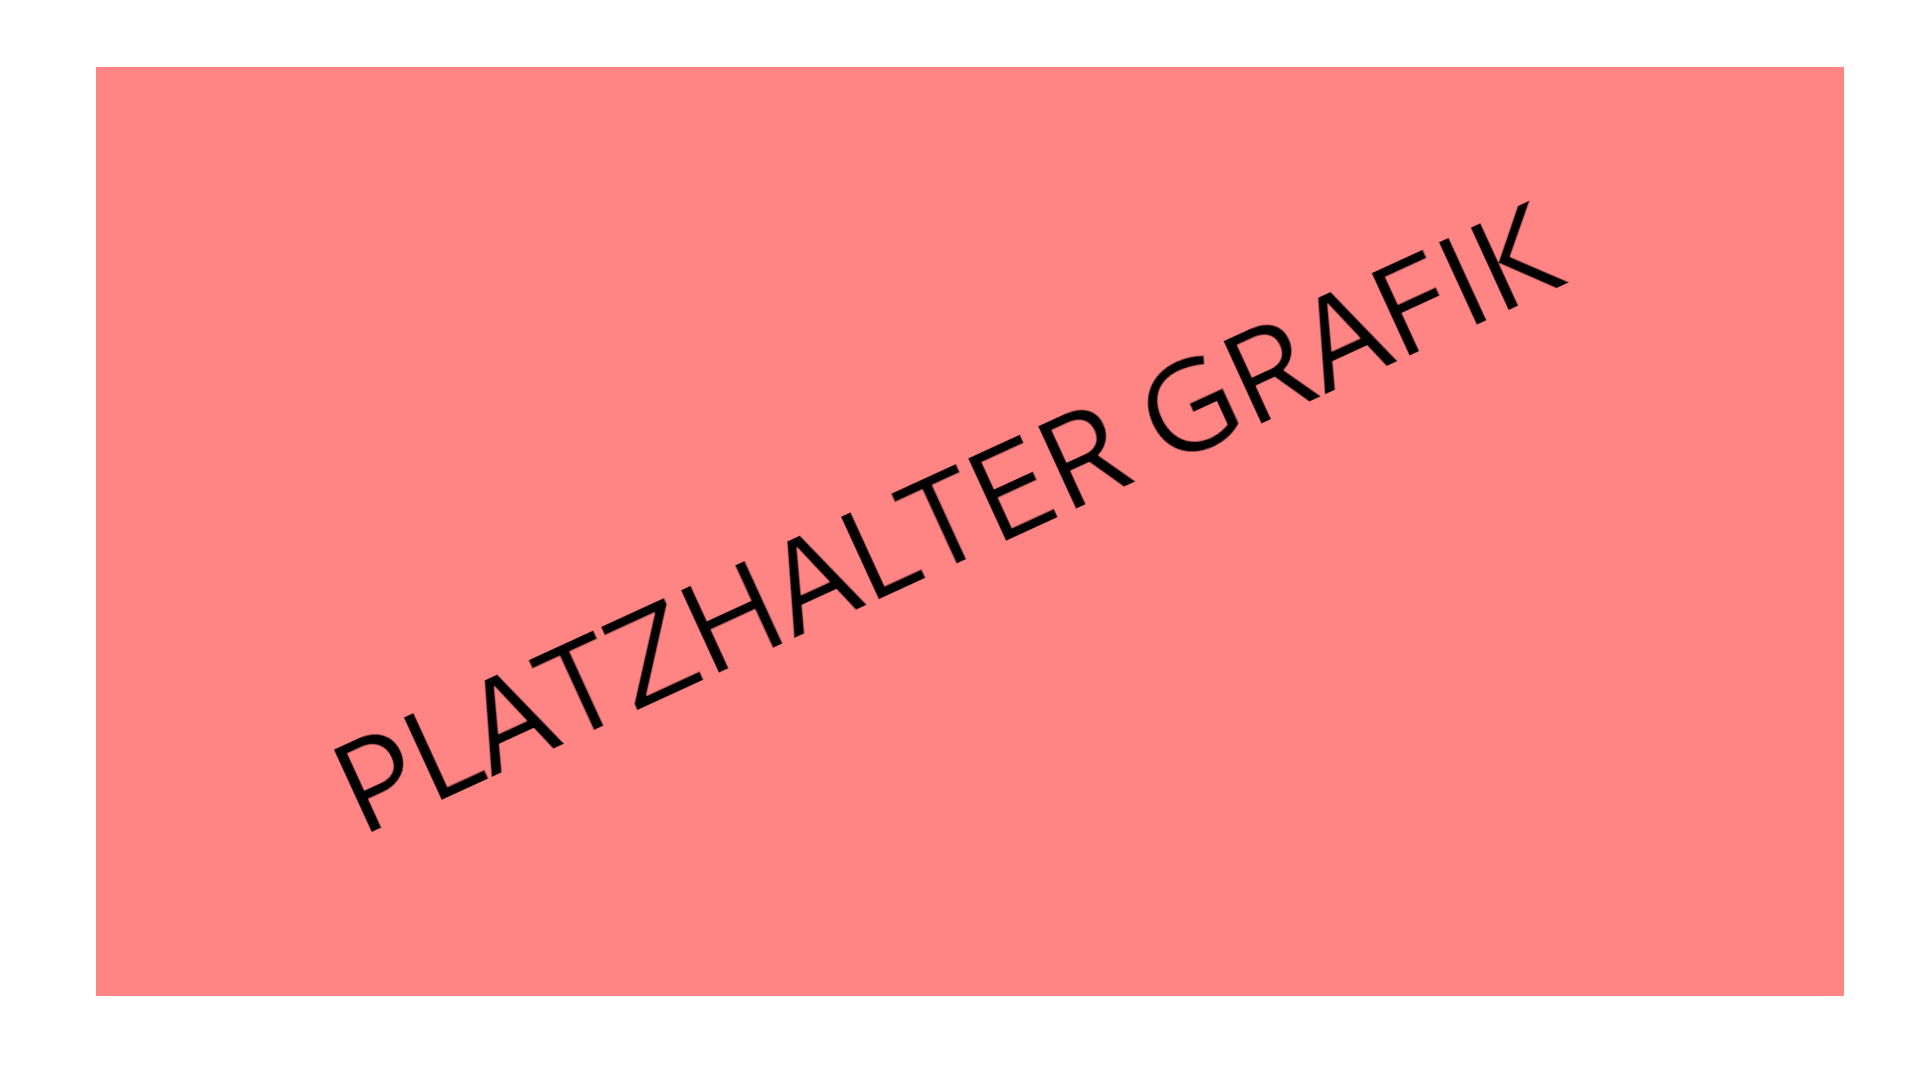
\includegraphics[height=6cm]{bilder/todo.png}
\captionof{figure}{Metamodell - Klassenname}
\end{center}

Lorem ipsum dolor sit amet, consetetur sadipscing elitr, sed diam nonumy eirmod tempor invidunt ut labore et dolore magna aliquyam erat, sed diam voluptua. At vero eos et accusam et justo duo dolores et ea rebum. Stet clita kasd gubergren, no sea takimata sanctus est Lorem ipsum dolor sit amet. Lorem ipsum dolor sit amet, consetetur sadipscing elitr, sed diam nonumy eirmod tempor invidunt ut labore et dolore magna aliquyam erat, sed diam voluptua.

\paragraph{Shared Kernel}

%TODO Grafik machen
\begin{center}
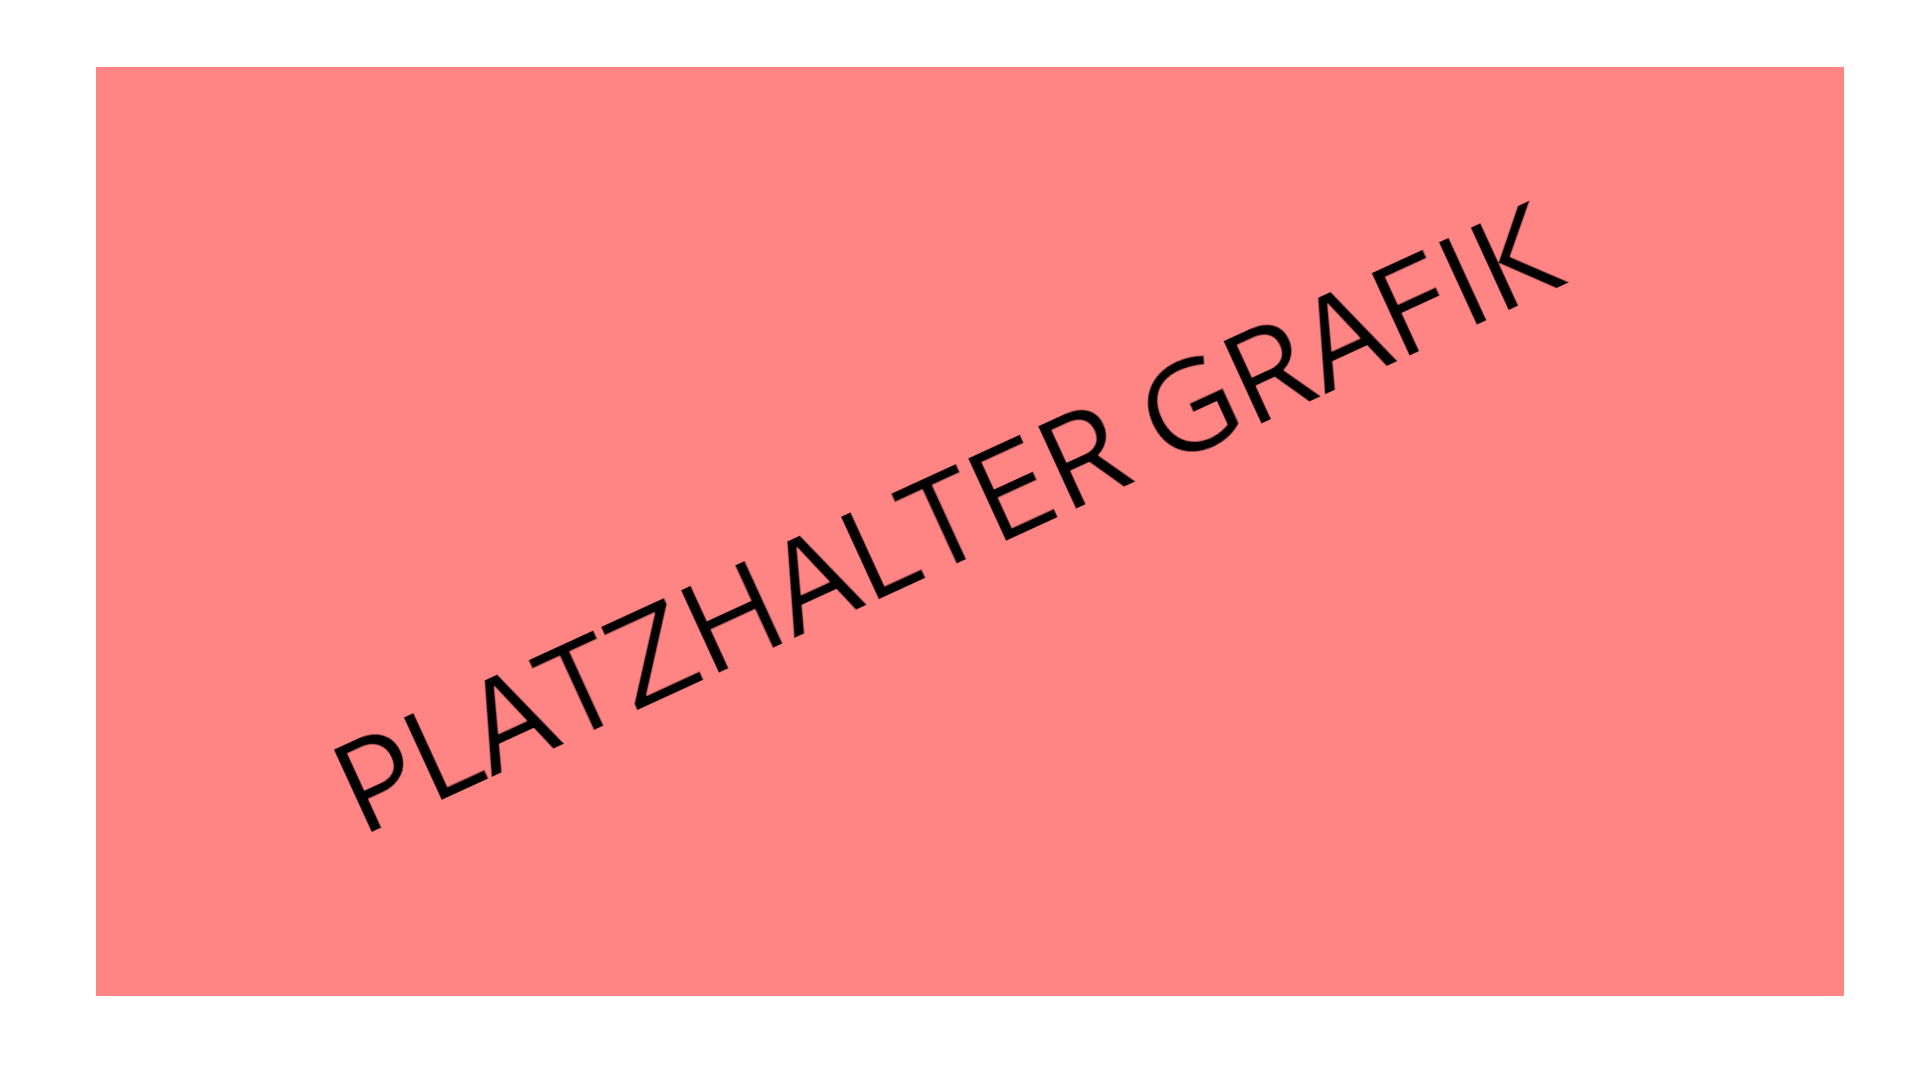
\includegraphics[height=6cm]{bilder/todo.png}
\captionof{figure}{Metamodell - Klassenname}
\end{center}

Lorem ipsum dolor sit amet, consetetur sadipscing elitr, sed diam nonumy eirmod tempor invidunt ut labore et dolore magna aliquyam erat, sed diam voluptua. At vero eos et accusam et justo duo dolores et ea rebum. Stet clita kasd gubergren, no sea takimata sanctus est Lorem ipsum dolor sit amet. Lorem ipsum dolor sit amet, consetetur sadipscing elitr, sed diam nonumy eirmod tempor invidunt ut labore et dolore magna aliquyam erat, sed diam voluptua.

\newpage
\paragraph{Customer/Supplier}

%TODO Grafik machen
\begin{center}
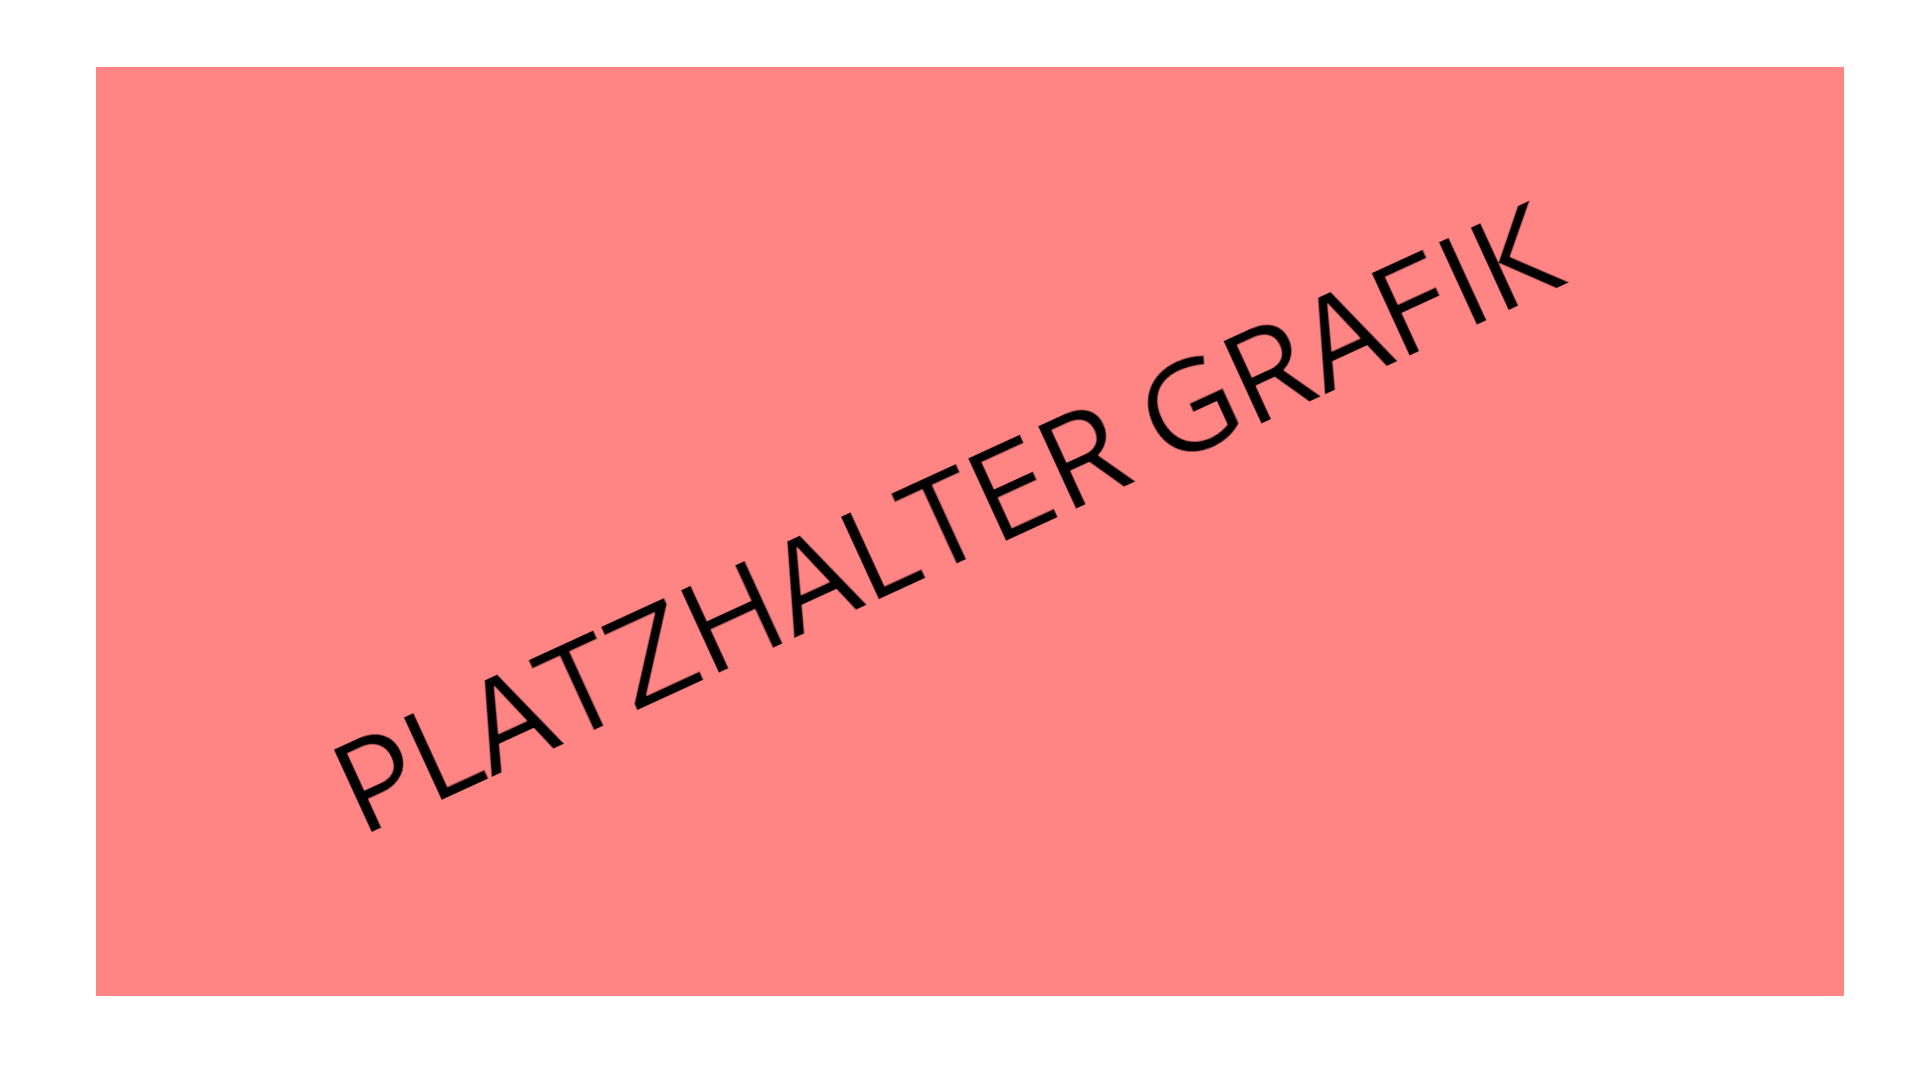
\includegraphics[height=6cm]{bilder/todo.png}
\captionof{figure}{Metamodell - Klassenname}
\end{center}

Lorem ipsum dolor sit amet, consetetur sadipscing elitr, sed diam nonumy eirmod tempor invidunt ut labore et dolore magna aliquyam erat, sed diam voluptua. At vero eos et accusam et justo duo dolores et ea rebum. Stet clita kasd gubergren, no sea takimata sanctus est Lorem ipsum dolor sit amet. Lorem ipsum dolor sit amet, consetetur sadipscing elitr, sed diam nonumy eirmod tempor invidunt ut labore et dolore magna aliquyam erat, sed diam voluptua.

\paragraph{Conformist}

%TODO Grafik machen
\begin{center}
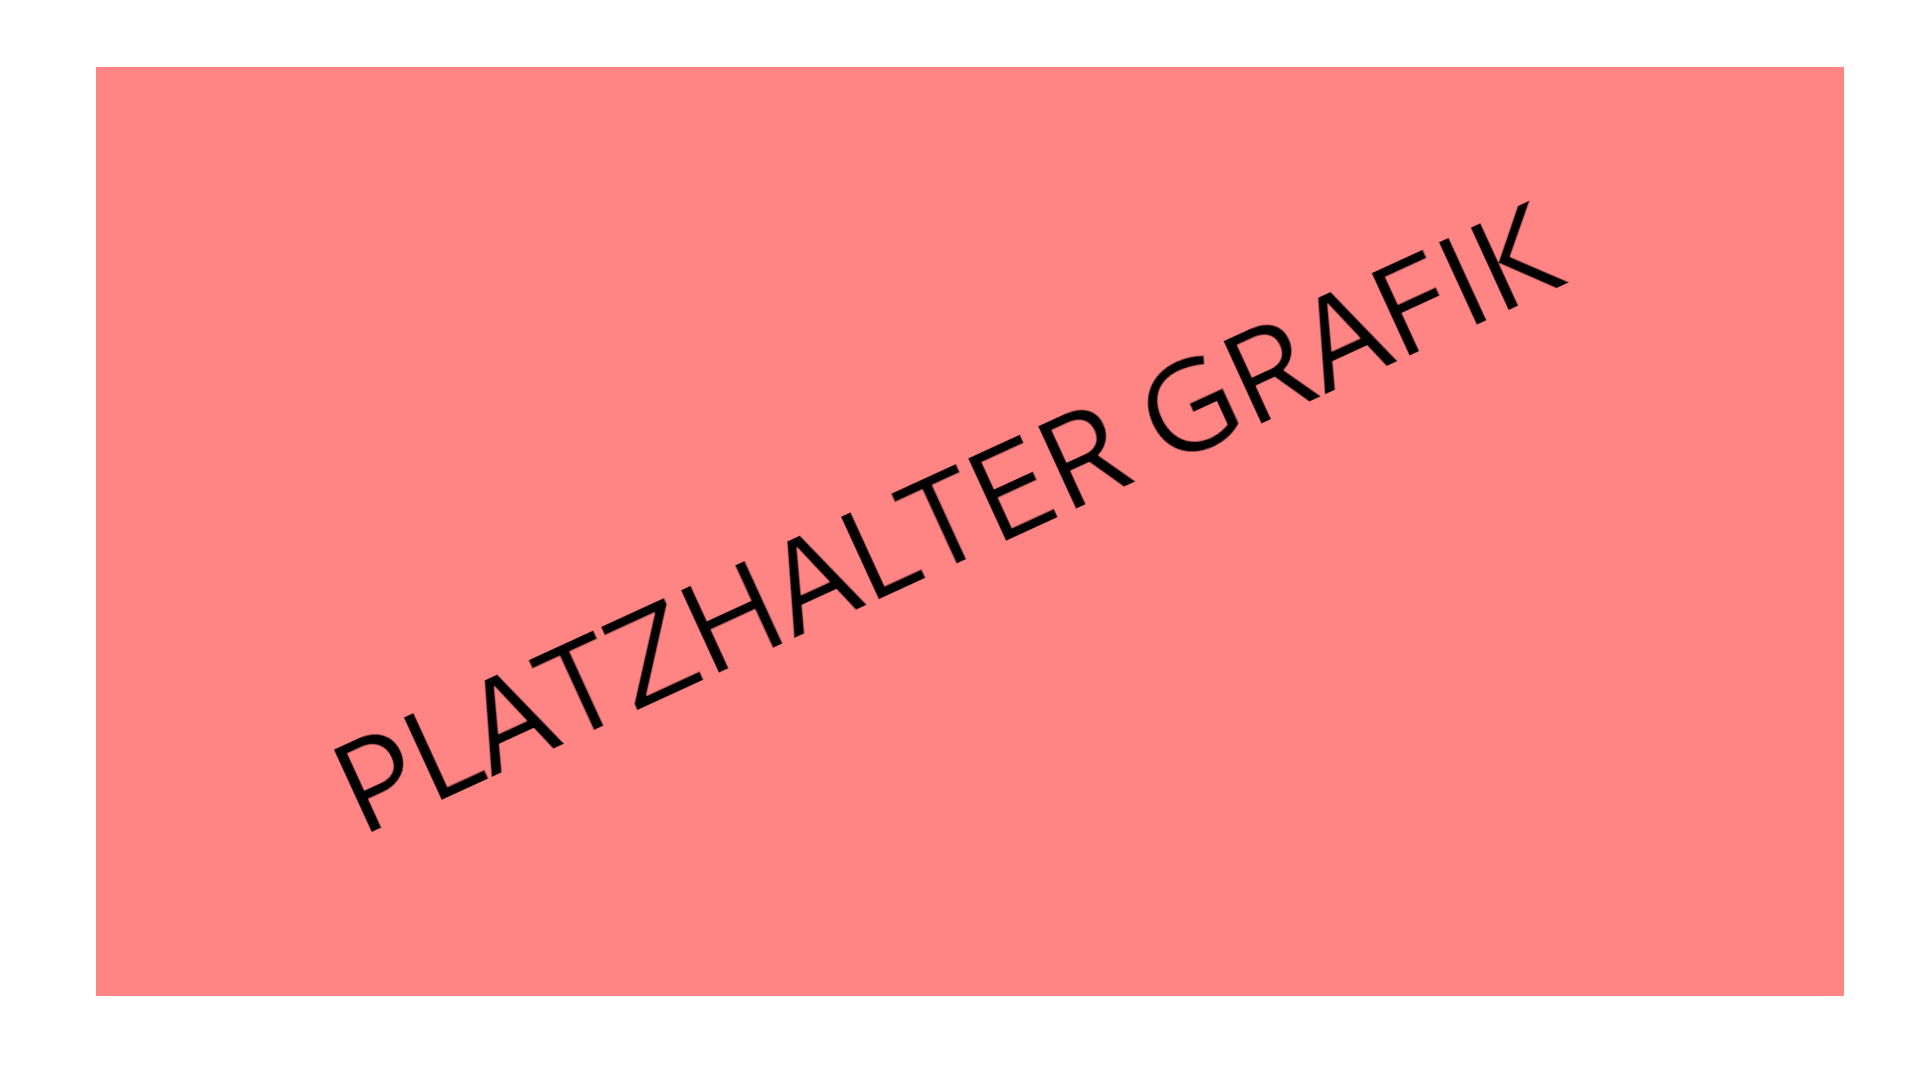
\includegraphics[height=6cm]{bilder/todo.png}
\captionof{figure}{Metamodell - Klassenname}
\end{center}

Lorem ipsum dolor sit amet, consetetur sadipscing elitr, sed diam nonumy eirmod tempor invidunt ut labore et dolore magna aliquyam erat, sed diam voluptua. At vero eos et accusam et justo duo dolores et ea rebum. Stet clita kasd gubergren, no sea takimata sanctus est Lorem ipsum dolor sit amet. Lorem ipsum dolor sit amet, consetetur sadipscing elitr, sed diam nonumy eirmod tempor invidunt ut labore et dolore magna aliquyam erat, sed diam voluptua.

\newpage
\paragraph{Anticorruption Layer}

%TODO Grafik machen
\begin{center}
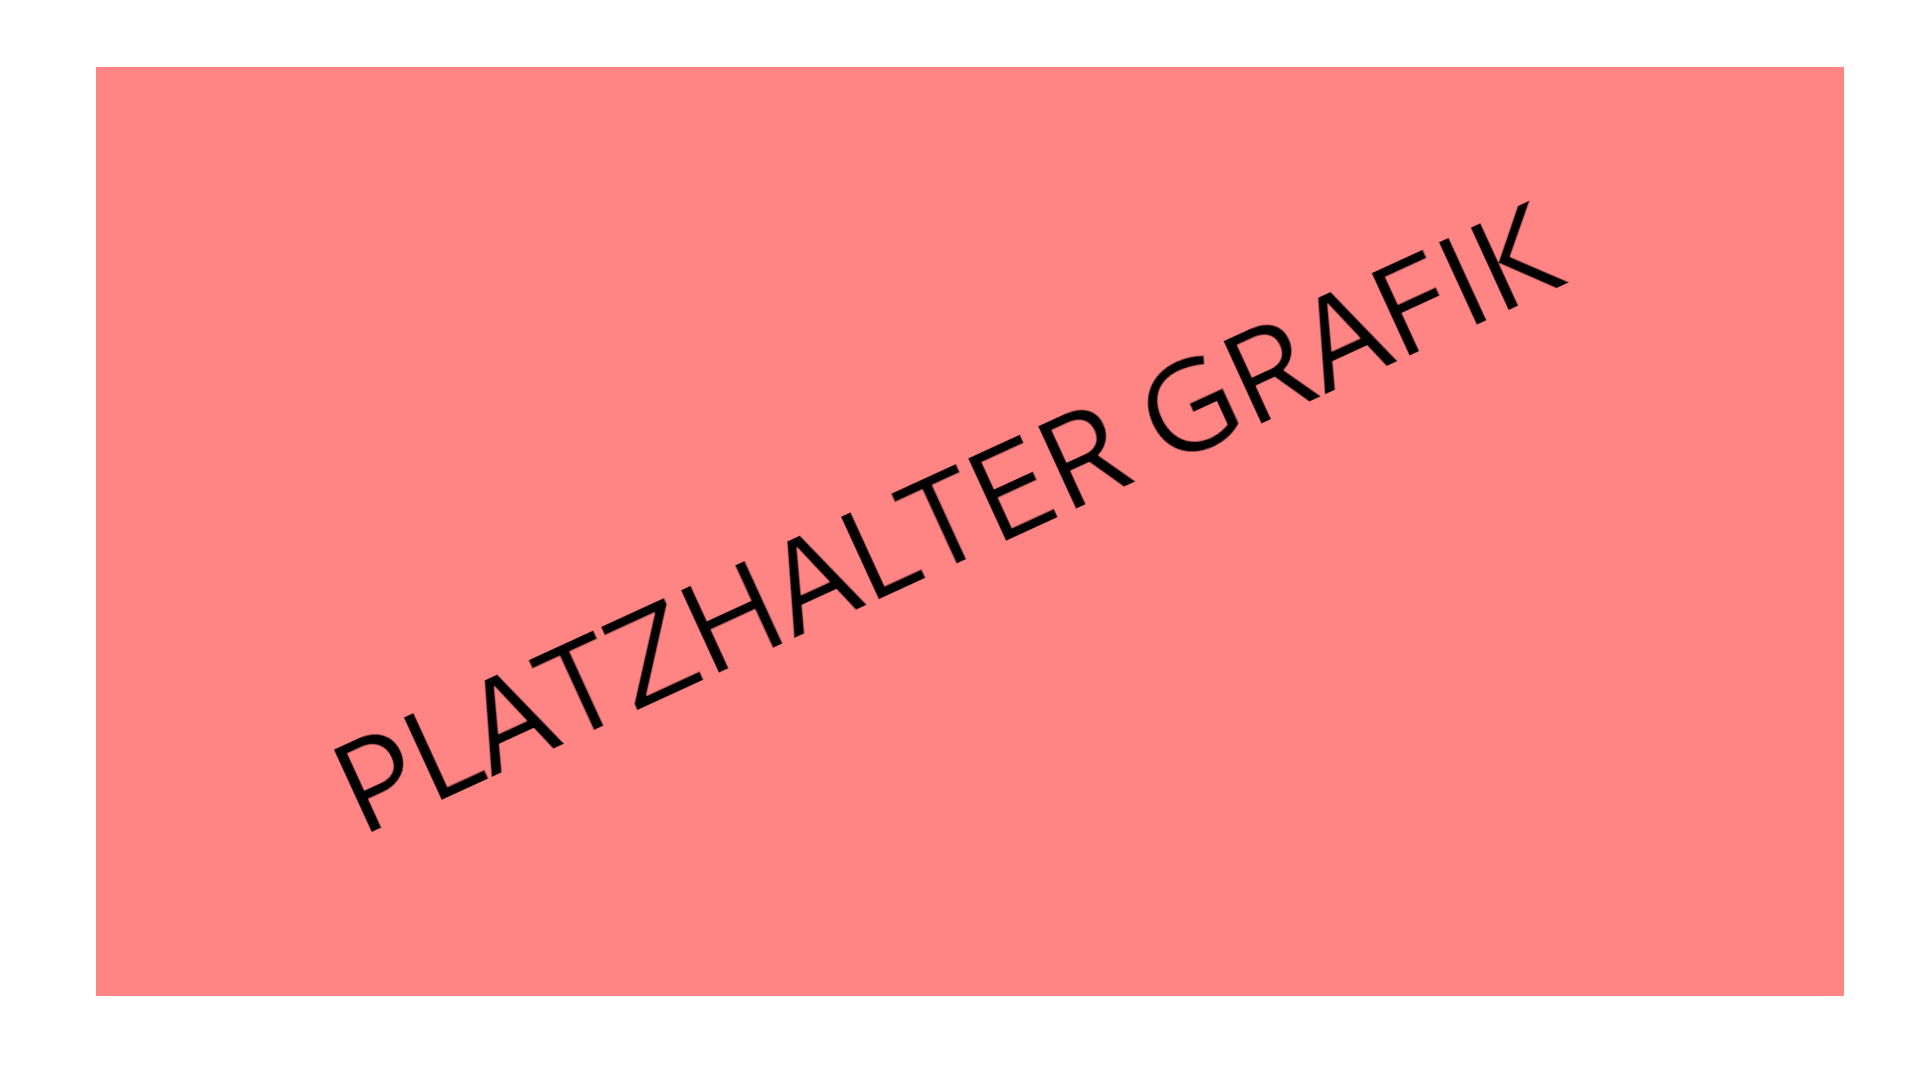
\includegraphics[height=6cm]{bilder/todo.png}
\captionof{figure}{Metamodell - Klassenname}
\end{center}

Lorem ipsum dolor sit amet, consetetur sadipscing elitr, sed diam nonumy eirmod tempor invidunt ut labore et dolore magna aliquyam erat, sed diam voluptua. At vero eos et accusam et justo duo dolores et ea rebum. Stet clita kasd gubergren, no sea takimata sanctus est Lorem ipsum dolor sit amet. Lorem ipsum dolor sit amet, consetetur sadipscing elitr, sed diam nonumy eirmod tempor invidunt ut labore et dolore magna aliquyam erat, sed diam voluptua.

\paragraph{Open Host Service}

%TODO Grafik machen
\begin{center}
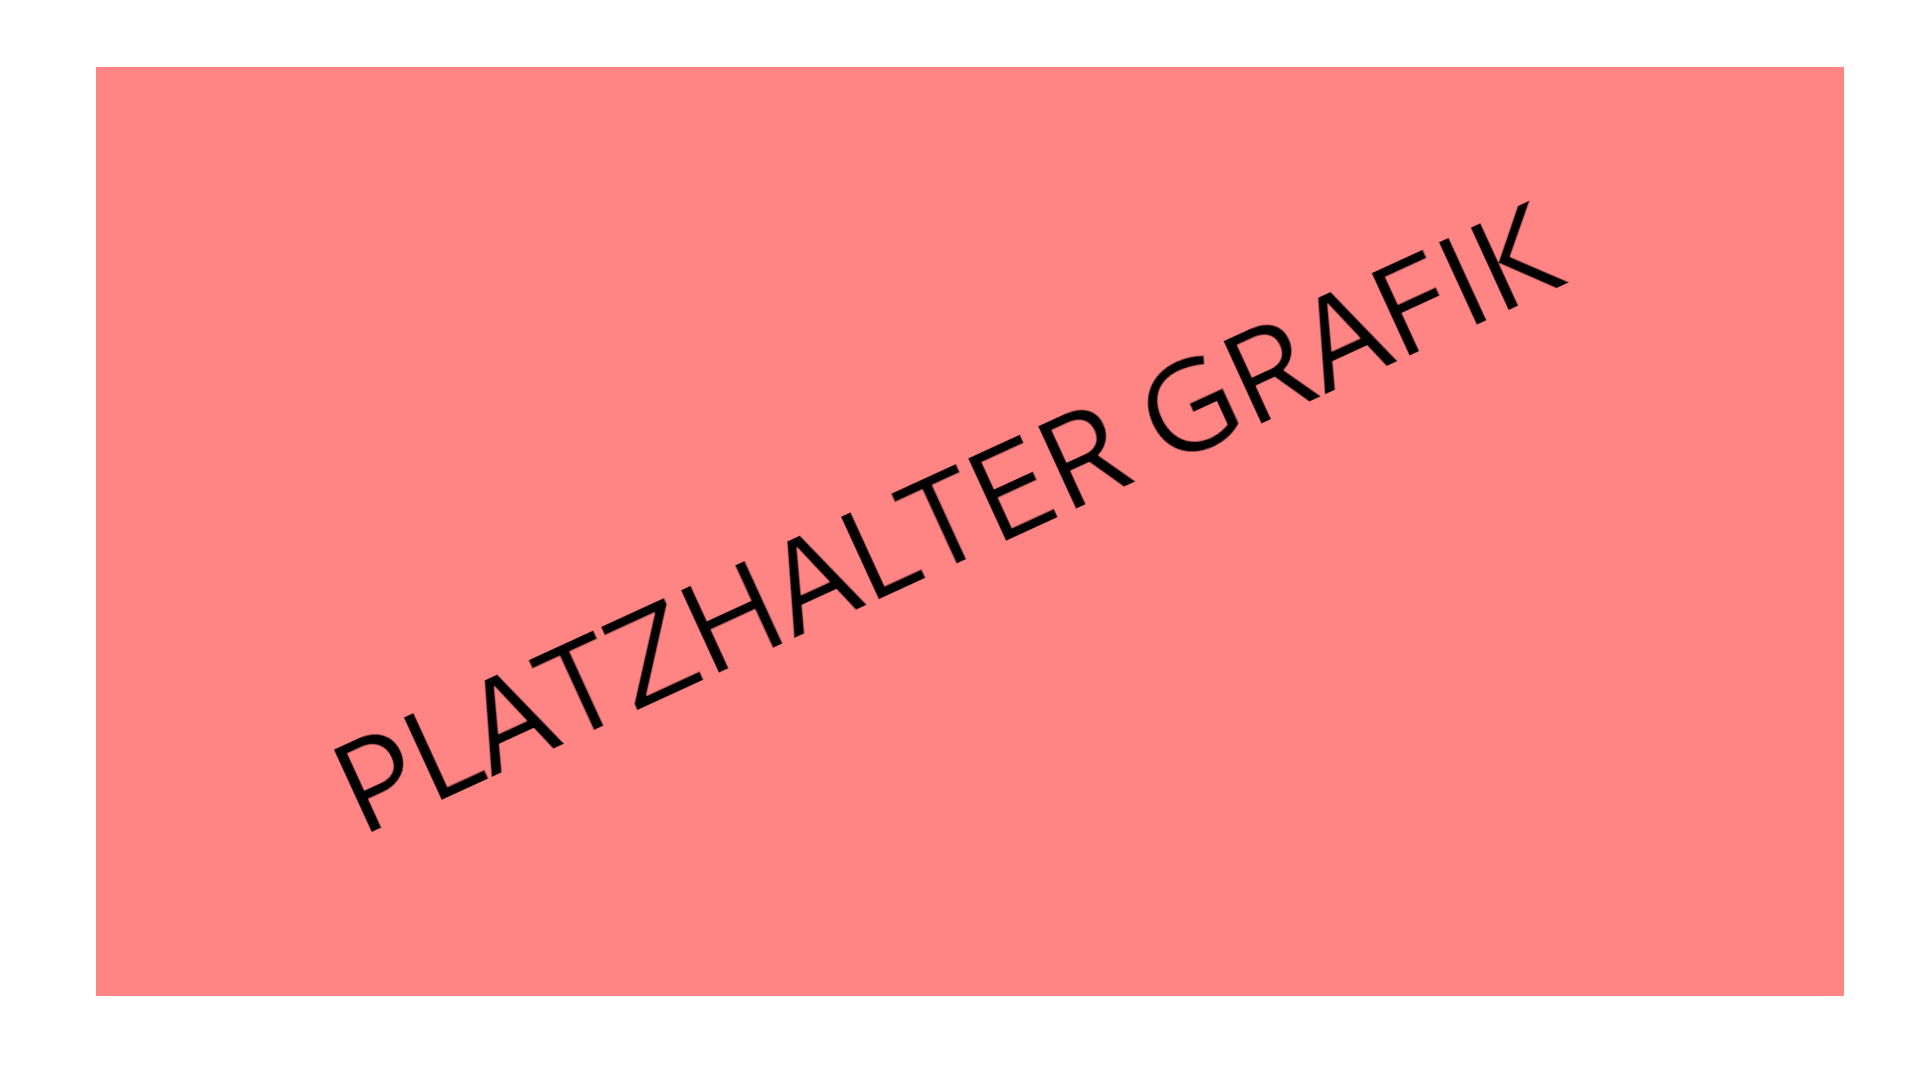
\includegraphics[height=6cm]{bilder/todo.png}
\captionof{figure}{Metamodell - Klassenname}
\end{center}

Lorem ipsum dolor sit amet, consetetur sadipscing elitr, sed diam nonumy eirmod tempor invidunt ut labore et dolore magna aliquyam erat, sed diam voluptua. At vero eos et accusam et justo duo dolores et ea rebum. Stet clita kasd gubergren, no sea takimata sanctus est Lorem ipsum dolor sit amet. Lorem ipsum dolor sit amet, consetetur sadipscing elitr, sed diam nonumy eirmod tempor invidunt ut labore et dolore magna aliquyam erat, sed diam voluptua.

\newpage
\paragraph{Published Language}

%TODO Grafik machen
\begin{center}
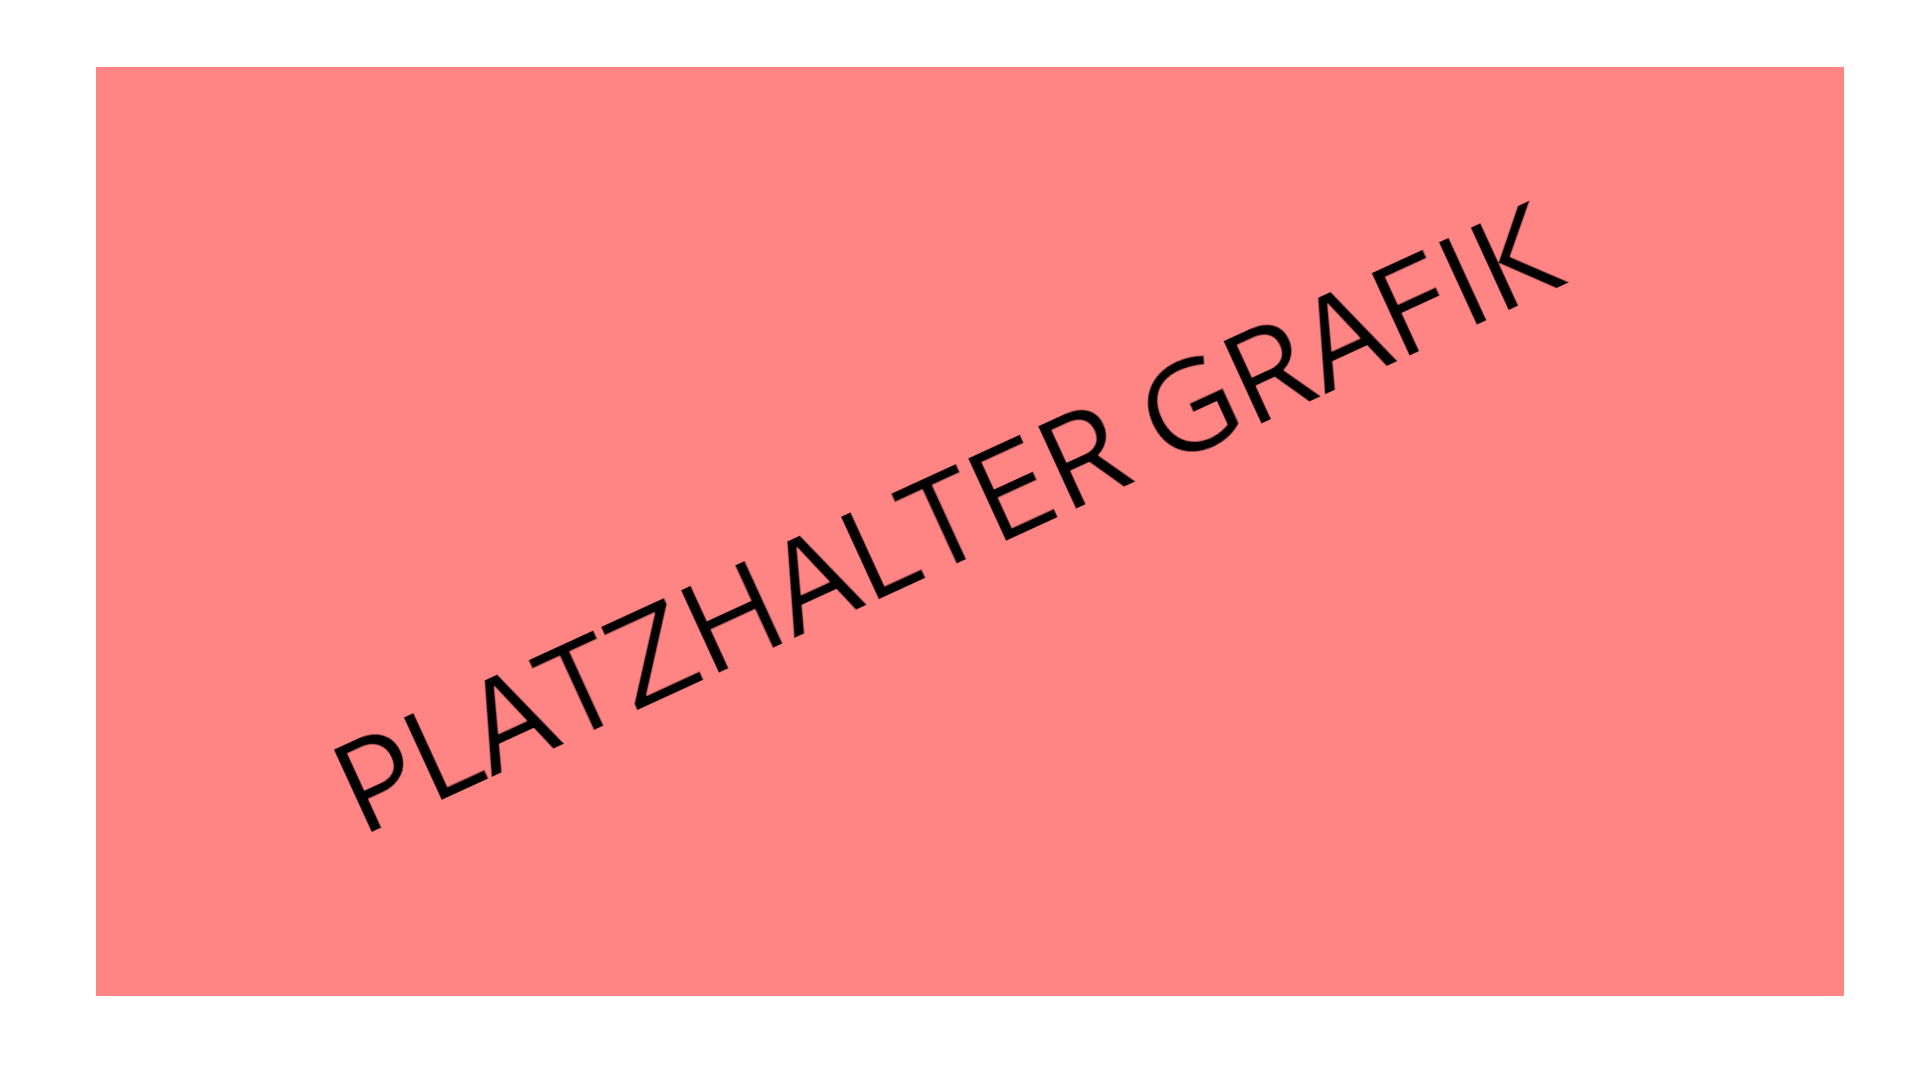
\includegraphics[height=6cm]{bilder/todo.png}
\captionof{figure}{Metamodell - Klassenname}
\end{center}

Lorem ipsum dolor sit amet, consetetur sadipscing elitr, sed diam nonumy eirmod tempor invidunt ut labore et dolore magna aliquyam erat, sed diam voluptua. At vero eos et accusam et justo duo dolores et ea rebum. Stet clita kasd gubergren, no sea takimata sanctus est Lorem ipsum dolor sit amet. Lorem ipsum dolor sit amet, consetetur sadipscing elitr, sed diam nonumy eirmod tempor invidunt ut labore et dolore magna aliquyam erat, sed diam voluptua.

\newpage
\paragraph{Gesamtüberblick}

\begin{center}
\rotatebox{90}{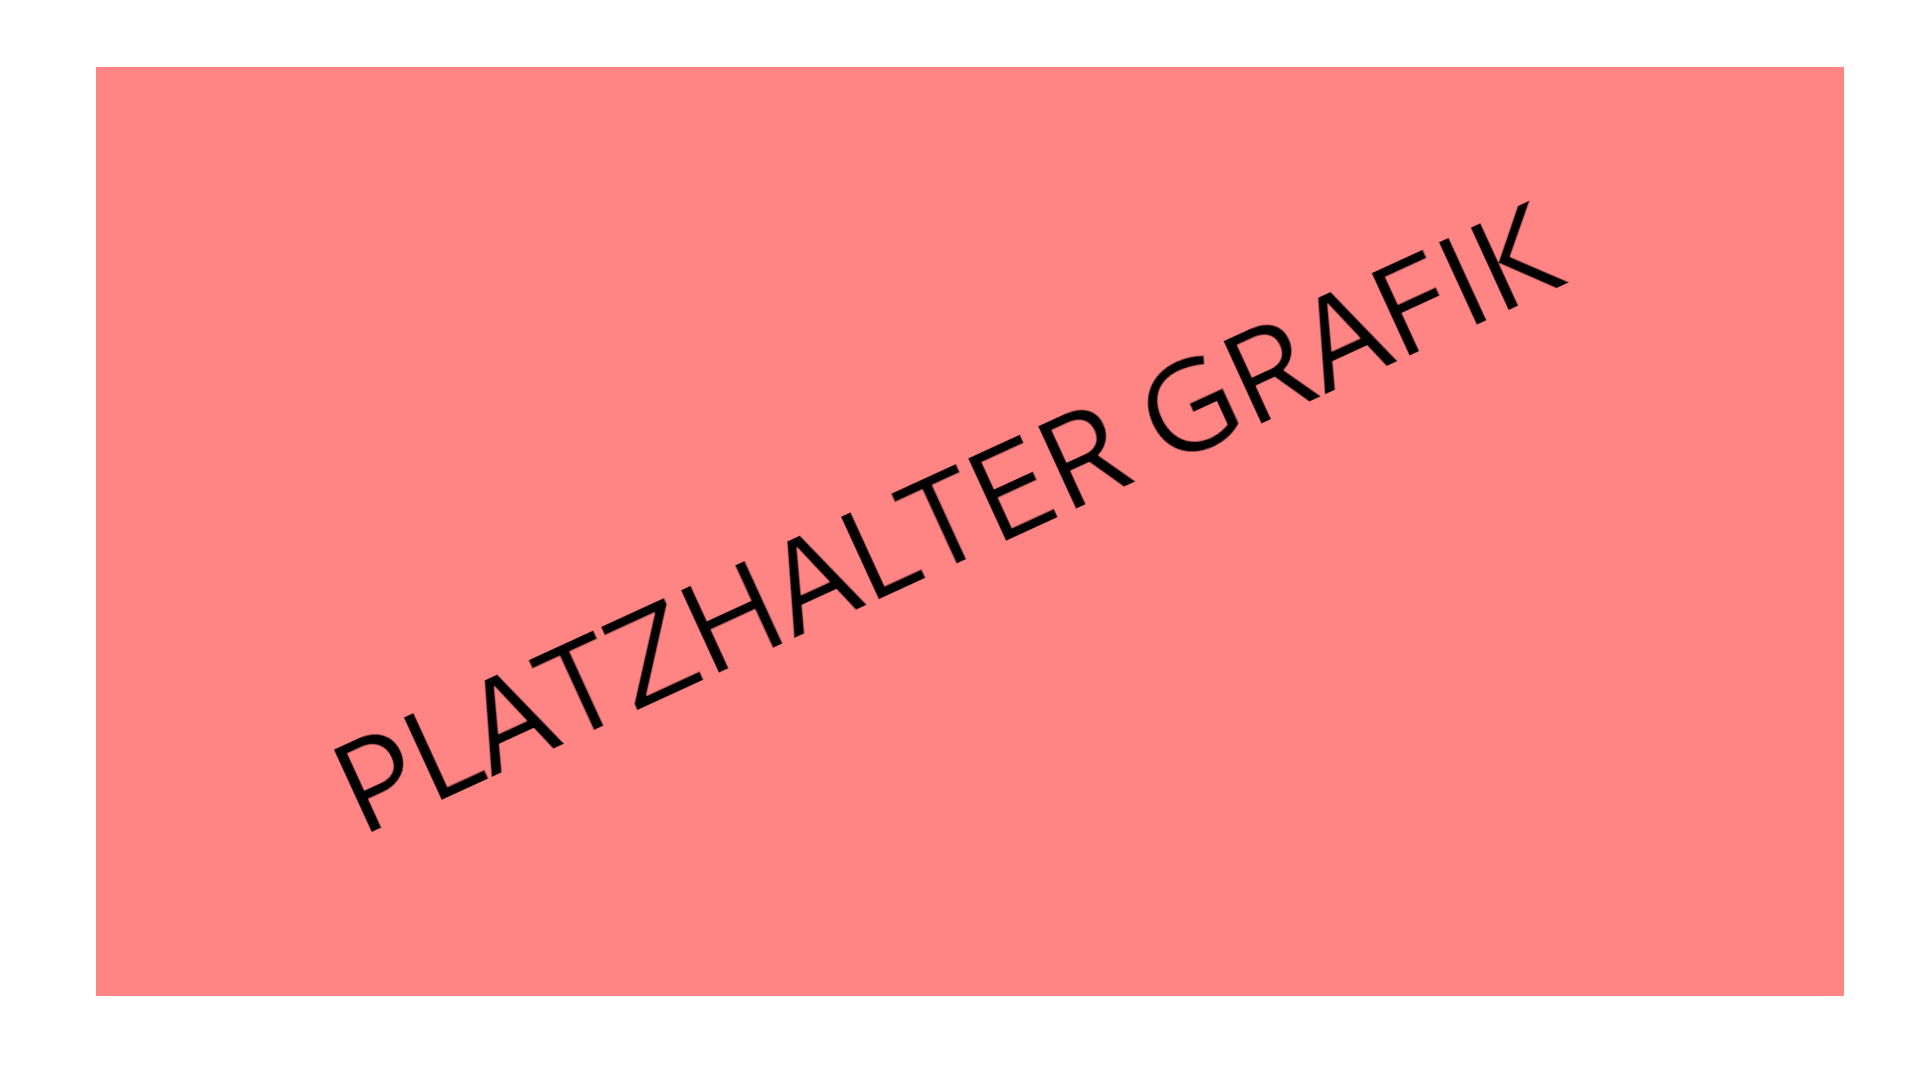
\includegraphics[height=10cm]{bilder/todo.png}}
\captionof{figure}{Metamodell - Klassenname}
\end{center}

%%%%%%%%%%%%%%%%%%%%%%%%%%%%%%%%%%%%%%%%%%%%%%%%%%%%%%%%%%%%%%%%%%%%%%%%%%%%%%%%%%%%%%%%%%%%%%%%%%%%%%%%%%%%%%%%%%%%
%			Infrastruktur
%%%%%%%%%%%%%%%%%%%%%%%%%%%%%%%%%%%%%%%%%%%%%%%%%%%%%%%%%%%%%%%%%%%%%%%%%%%%%%%%%%%%%%%%%%%%%%%%%%%%%%%%%%%%%%%%%%%%
\newpage
\subsection{Modellierung der Infrastrukturellen Umgebung}

\subsubsection{Abbildung Service Configuration}

\paragraph{Application.yml}

%TODO Grafik machen
\begin{center}
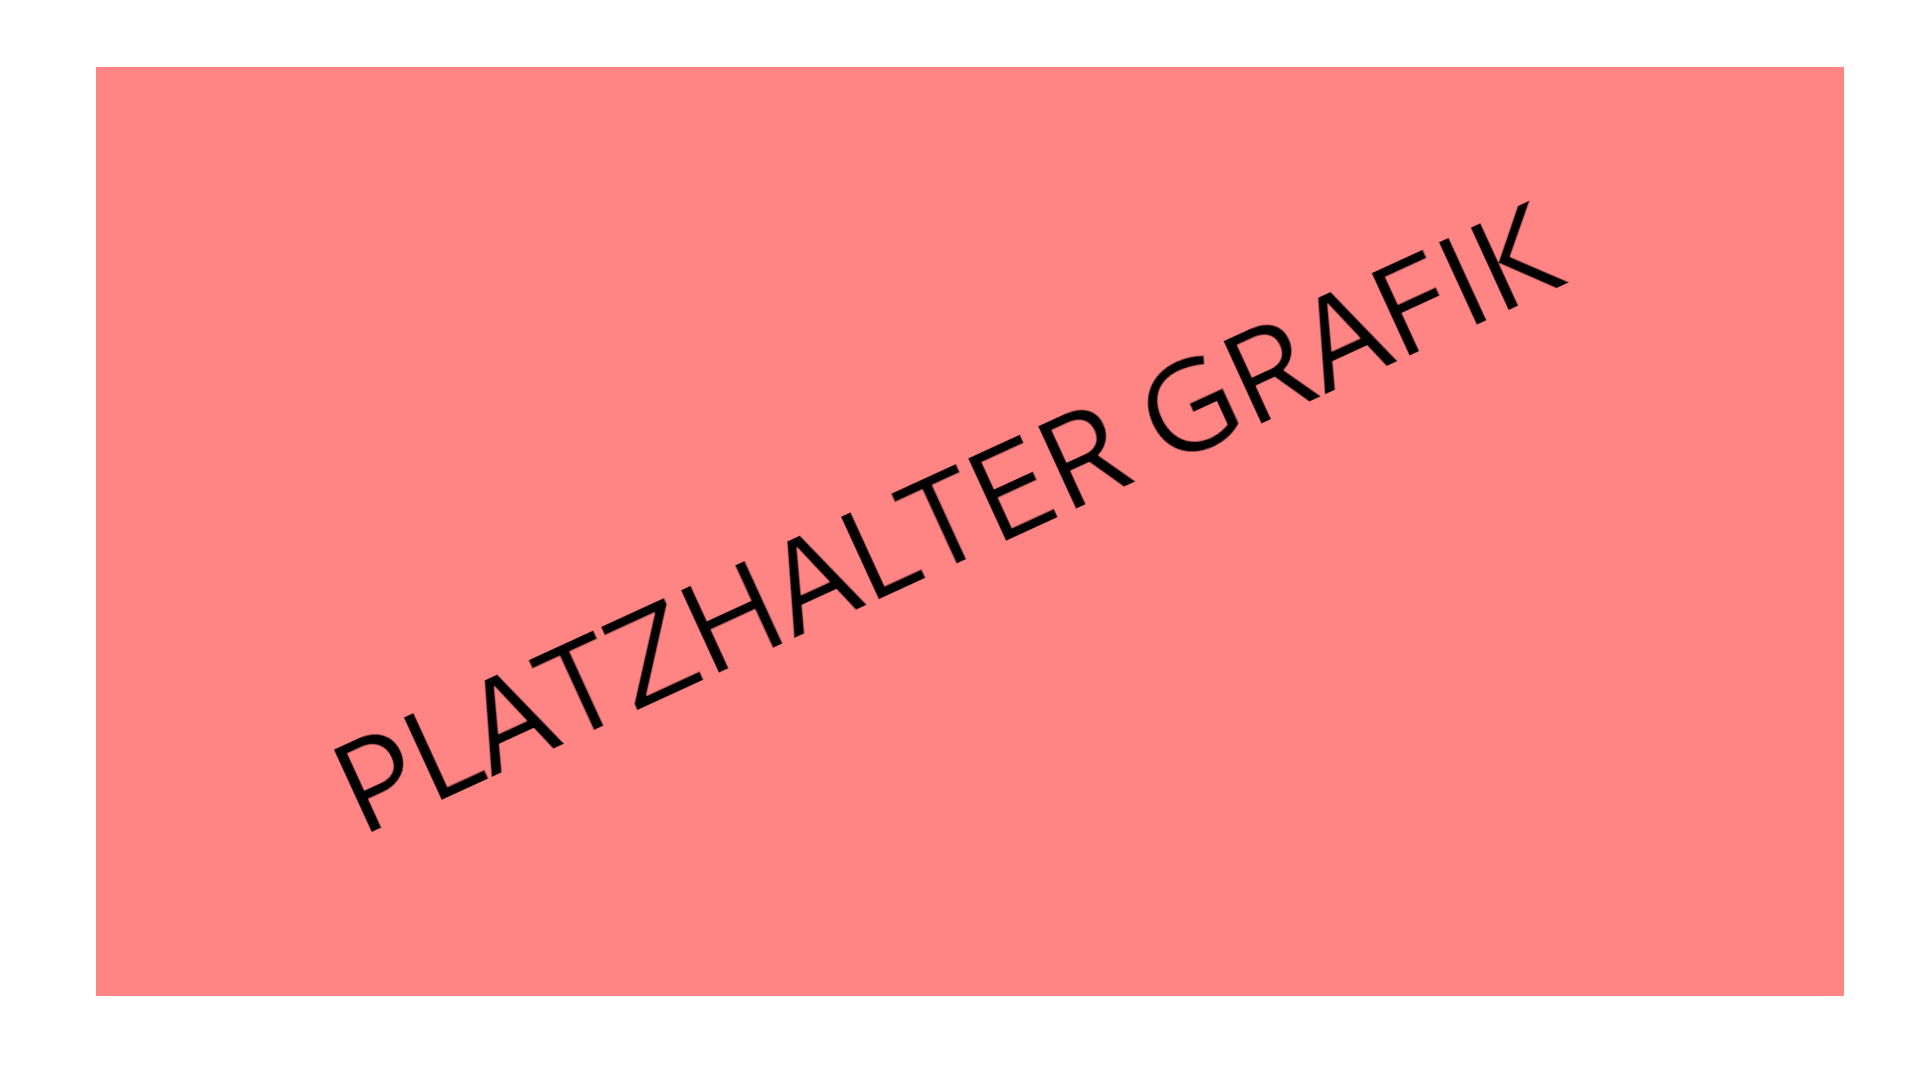
\includegraphics[height=6cm]{bilder/todo.png}
\captionof{figure}{Metamodell - Klassenname}
\end{center}

Lorem ipsum dolor sit amet, consetetur sadipscing elitr, sed diam nonumy eirmod tempor invidunt ut labore et dolore magna aliquyam erat, sed diam voluptua. At vero eos et accusam et justo duo dolores et ea rebum. Stet clita kasd gubergren, no sea takimata sanctus est Lorem ipsum dolor sit amet. Lorem ipsum dolor sit amet, consetetur sadipscing elitr, sed diam nonumy eirmod tempor invidunt ut labore et dolore magna aliquyam erat, sed diam voluptua.

\newpage
\subsubsection{Abbildung der Build Automation}

\paragraph{Build.gradle}

%TODO Grafik machen
\begin{center}
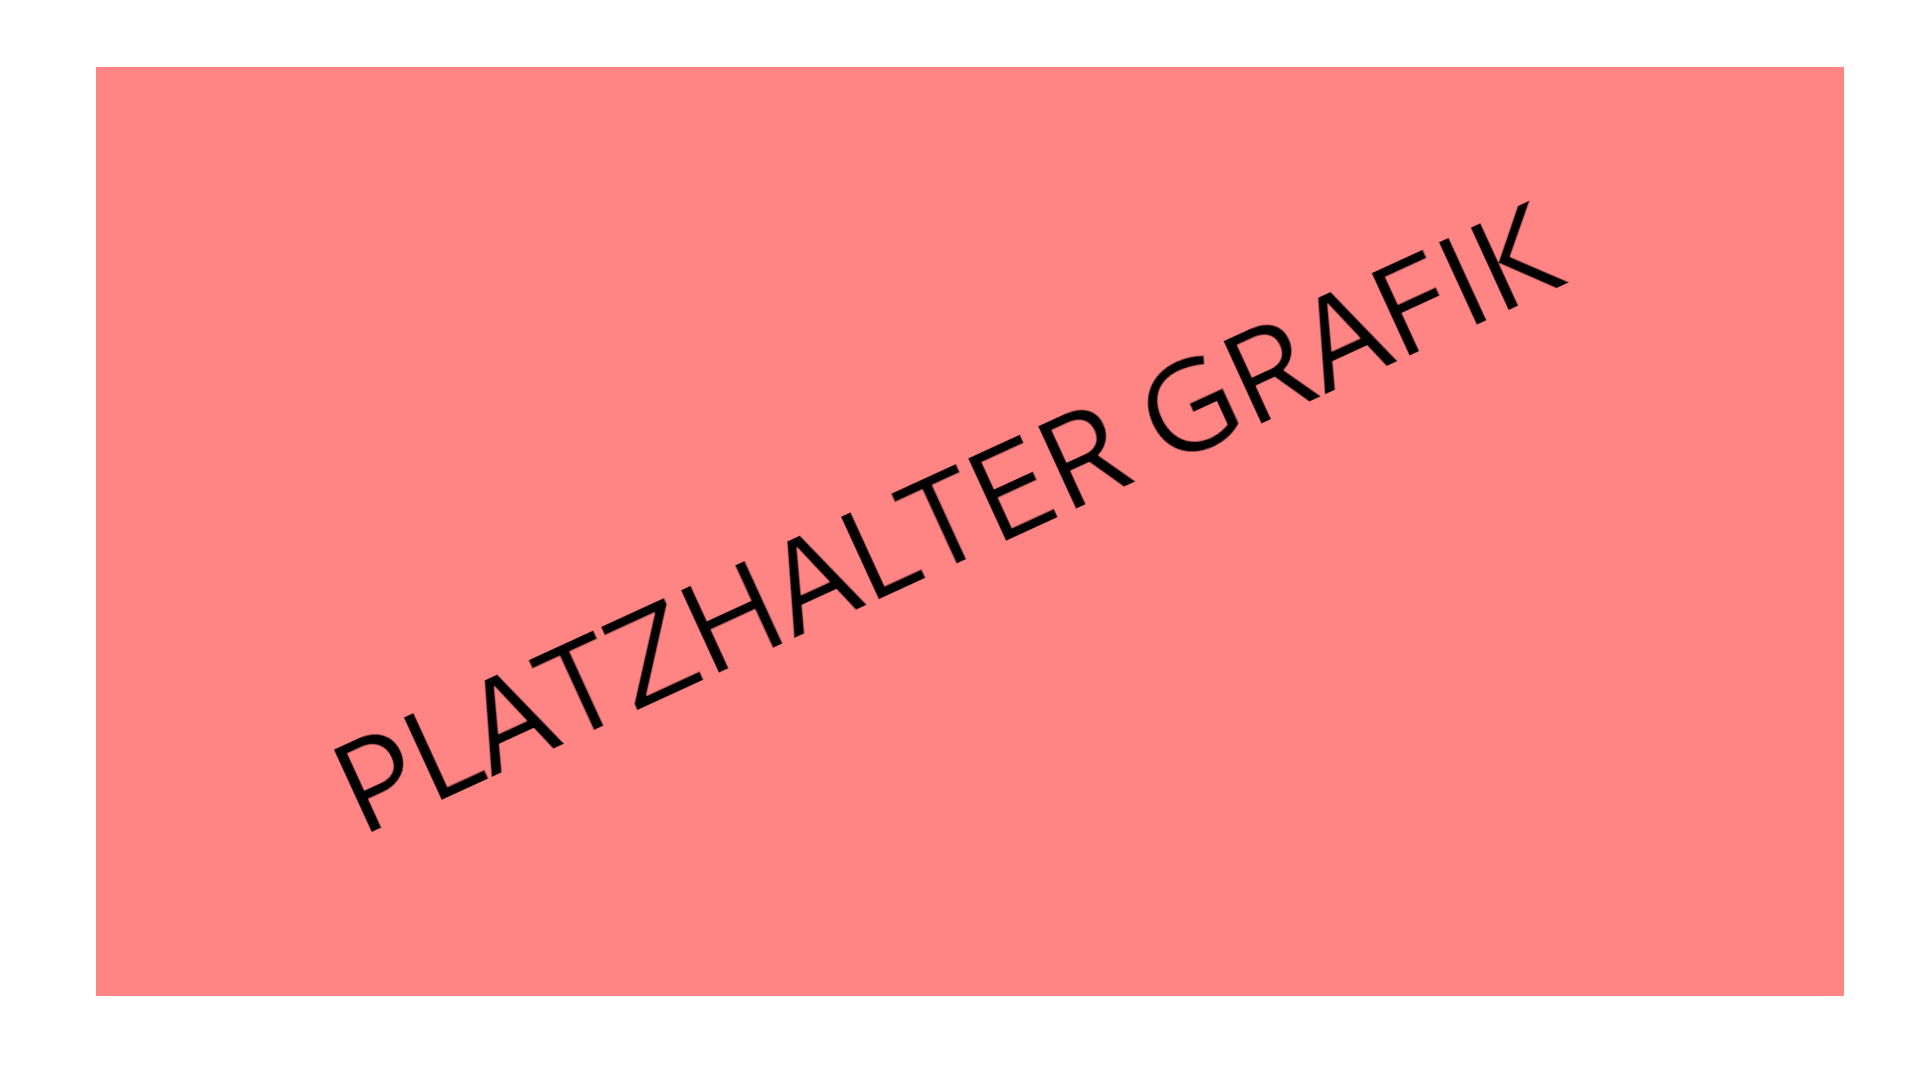
\includegraphics[height=6cm]{bilder/todo.png}
\captionof{figure}{Metamodell - Klassenname}
\end{center}

Lorem ipsum dolor sit amet, consetetur sadipscing elitr, sed diam nonumy eirmod tempor invidunt ut labore et dolore magna aliquyam erat, sed diam voluptua. At vero eos et accusam et justo duo dolores et ea rebum. Stet clita kasd gubergren, no sea takimata sanctus est Lorem ipsum dolor sit amet. Lorem ipsum dolor sit amet, consetetur sadipscing elitr, sed diam nonumy eirmod tempor invidunt ut labore et dolore magna aliquyam erat, sed diam voluptua.

\newpage
\paragraph{GitHubAction}

%TODO Grafik machen
\begin{center}
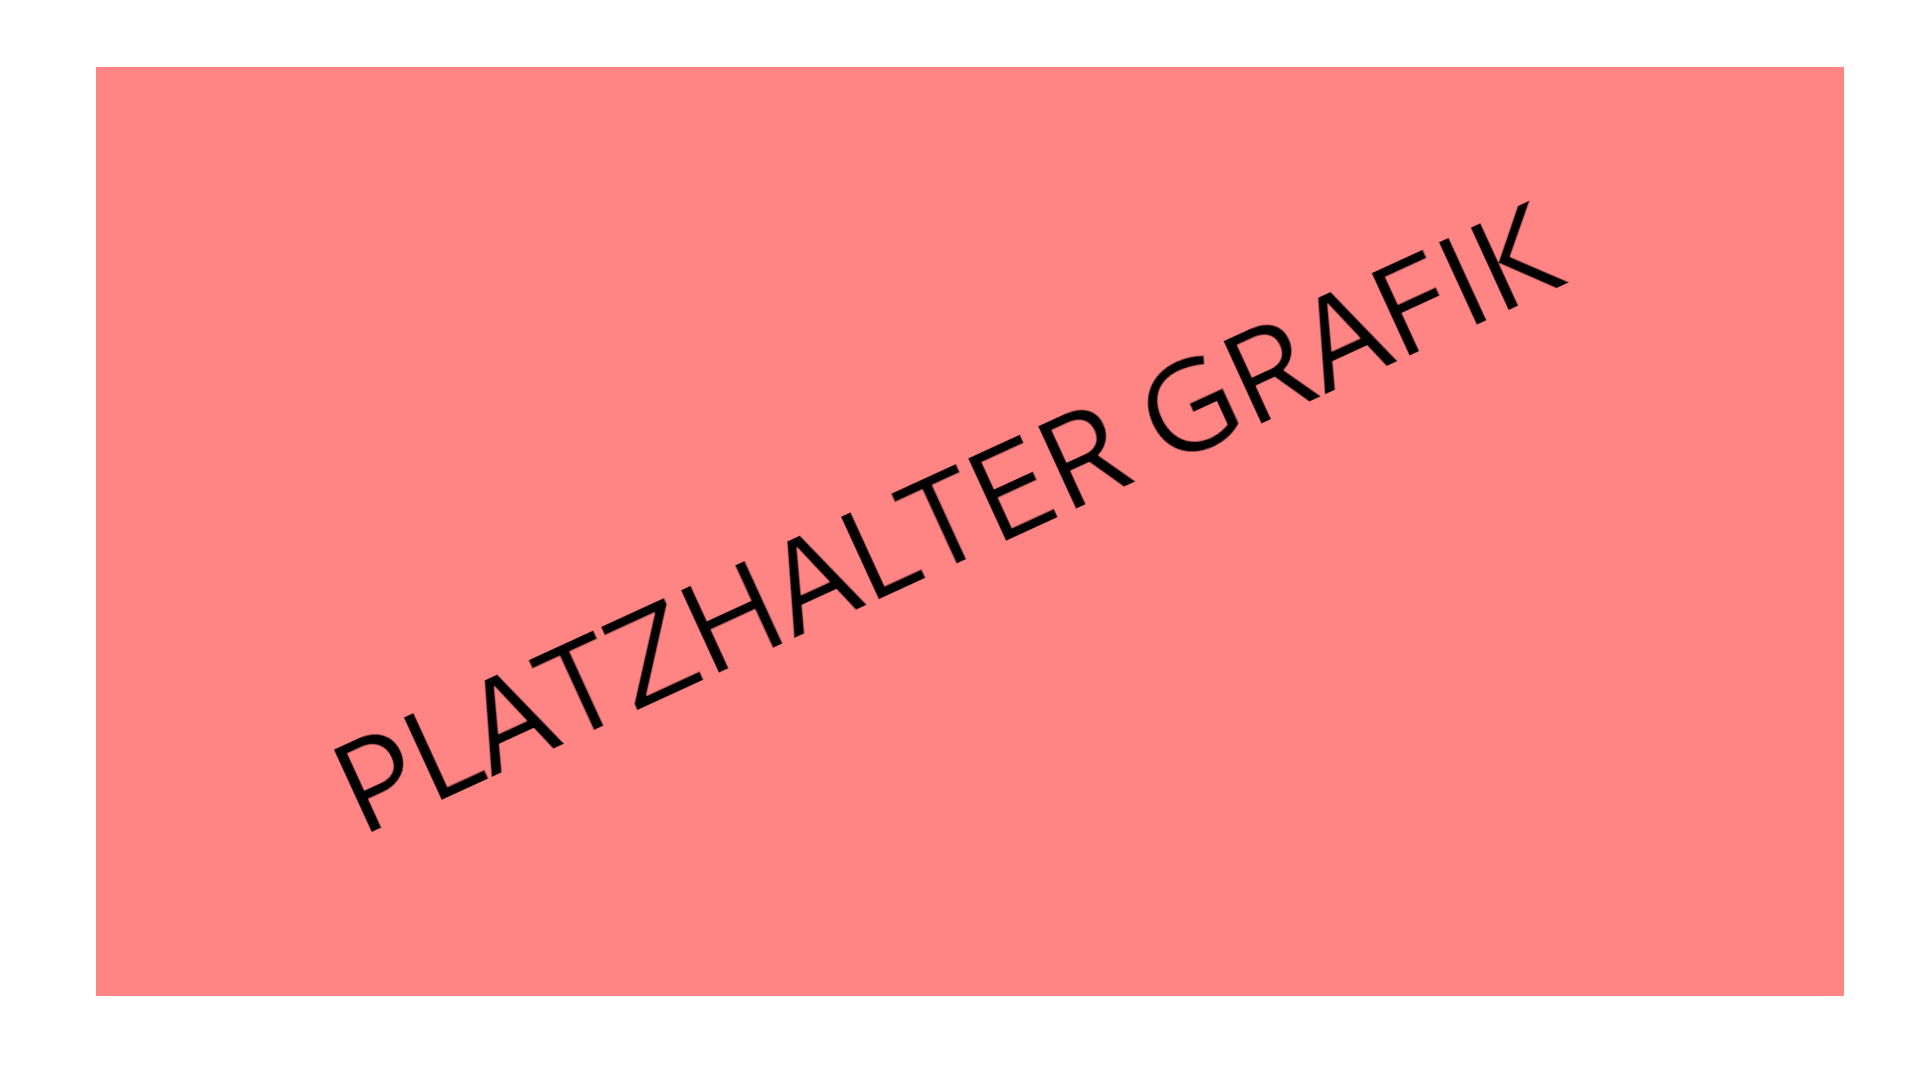
\includegraphics[height=6cm]{bilder/todo.png}
\captionof{figure}{Metamodell - Klassenname}
\end{center}

Lorem ipsum dolor sit amet, consetetur sadipscing elitr, sed diam nonumy eirmod tempor invidunt ut labore et dolore magna aliquyam erat, sed diam voluptua. At vero eos et accusam et justo duo dolores et ea rebum. Stet clita kasd gubergren, no sea takimata sanctus est Lorem ipsum dolor sit amet. Lorem ipsum dolor sit amet, consetetur sadipscing elitr, sed diam nonumy eirmod tempor invidunt ut labore et dolore magna aliquyam erat, sed diam voluptua.

\newpage
\subsubsection{Abbildung des Cloud Umgebung}

\paragraph{Deployement Abstraktion}

%TODO Grafik machen
\begin{center}
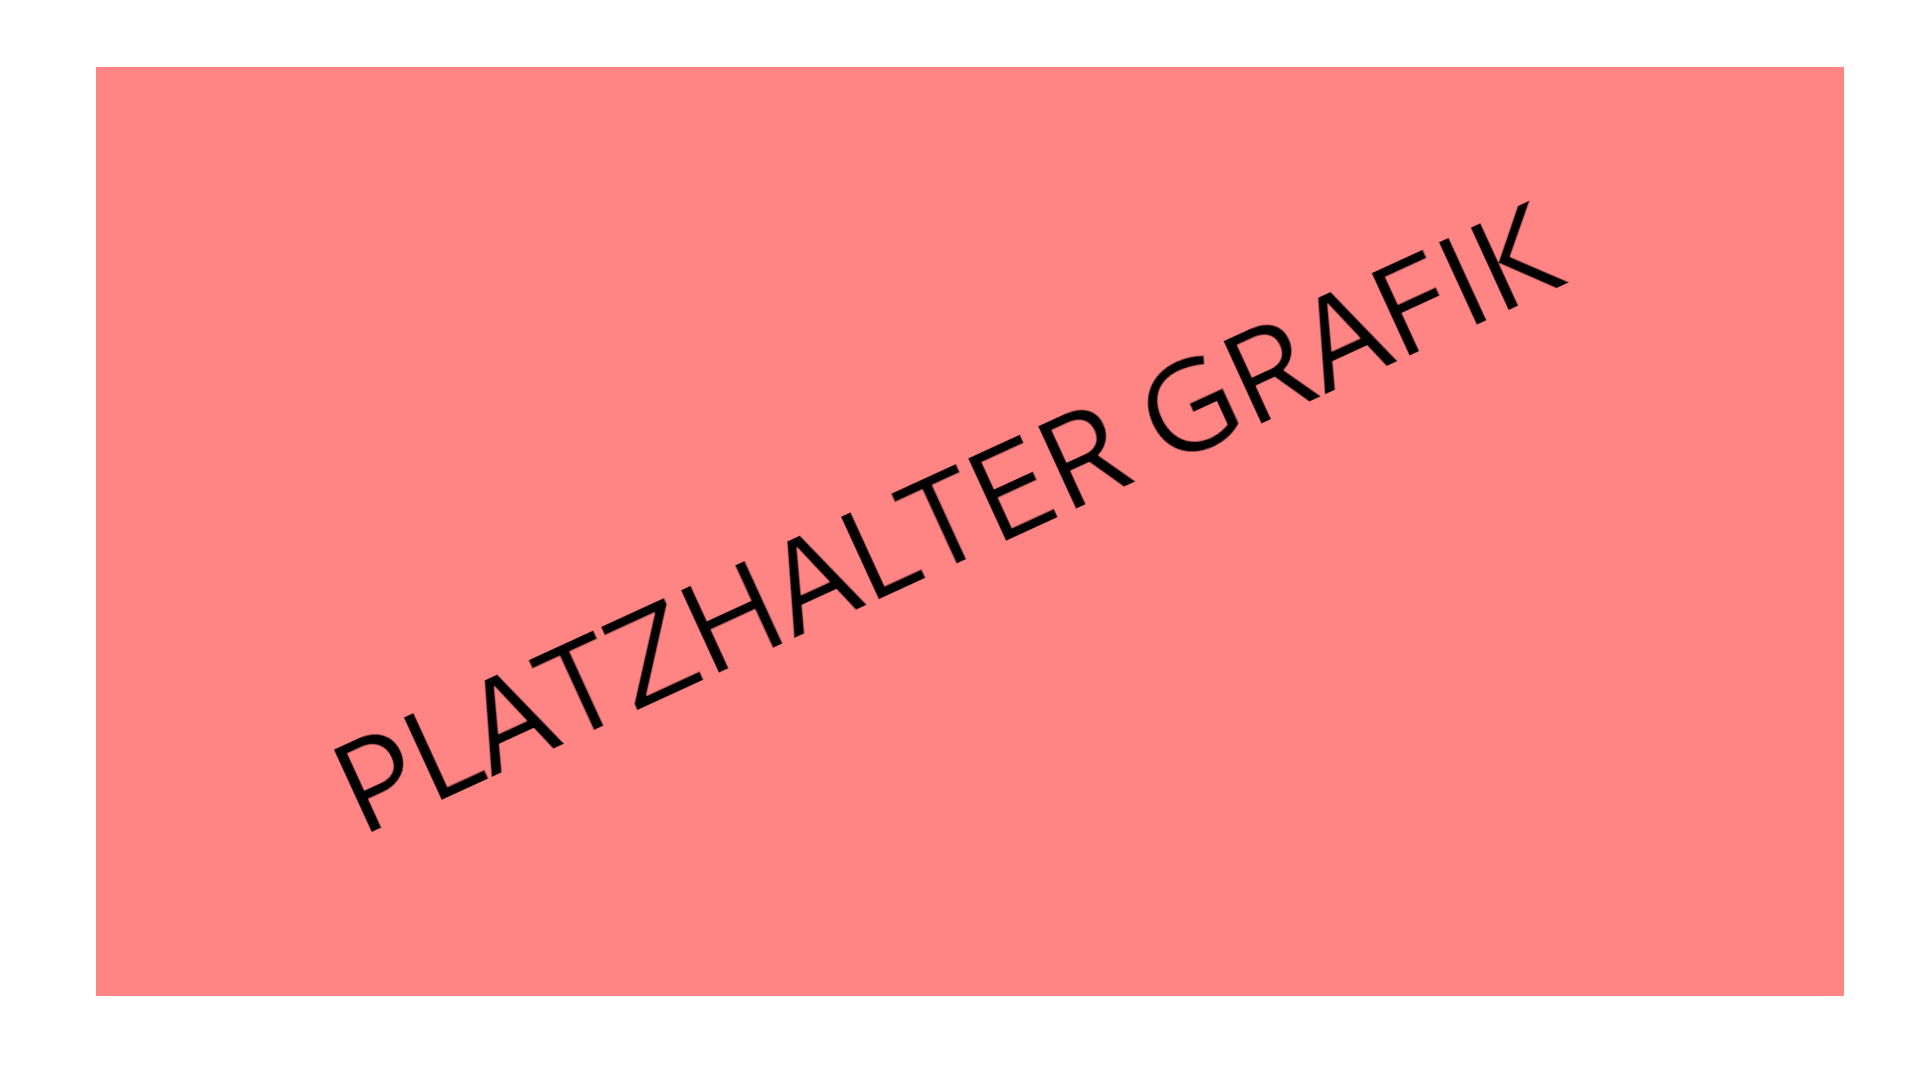
\includegraphics[height=6cm]{bilder/todo.png}
\captionof{figure}{Metamodell - Klassenname}
\end{center}

Lorem ipsum dolor sit amet, consetetur sadipscing elitr, sed diam nonumy eirmod tempor invidunt ut labore et dolore magna aliquyam erat, sed diam voluptua. At vero eos et accusam et justo duo dolores et ea rebum. Stet clita kasd gubergren, no sea takimata sanctus est Lorem ipsum dolor sit amet. Lorem ipsum dolor sit amet, consetetur sadipscing elitr, sed diam nonumy eirmod tempor invidunt ut labore et dolore magna aliquyam erat, sed diam voluptua.

\newpage
\subsection{Konzeption der konkreten Syntax}

